\documentclass{article}
\usepackage{graphicx} % Required for inserting images
\usepackage[french]{babel}
\usepackage[T1]{fontenc}
\usepackage[utf8]{inputenc}
\usepackage{amsmath}
\usepackage{txfonts}
\usepackage{color}
\usepackage{tikz}
\usepackage{url}
\usepackage{ulem}
\usepackage{caption}
\usepackage{subcaption}
\usepackage{tgpagella}
\usepackage[indent=20pt]{parskip}

\usepackage{geometry}
\geometry{
  a4paper,
  margin=25.4mm
}

\usepackage{lmodern,mathrsfs}
\usepackage{xparse}
\usepackage[inline,shortlabels]{enumitem}
\usepackage[most]{tcolorbox}
\tcbuselibrary{minted} % tcolorbox minted library, required to use the "minted" tcb listing engine (this library is not loaded by the option [most])
\usepackage{minted} % Allows input of raw code, such as Python code
\usepackage[colorlinks=true, linkcolor=blue, citecolor=green, urlcolor=cyan]{hyperref}

% Custom tcolorbox style for Python code (not the code or the box it appears in, just the options for the box)
\tcbset{
    pythoncodebox/.style={
        enhanced jigsaw,breakable,
        colback=gray!10,colframe=gray!20!black,
        boxrule=1pt,top=2pt,bottom=2pt,left=2pt,right=2pt,
        sharp corners,before skip=10pt,after skip=10pt,
        attach boxed title to top left,
        boxed title style={empty,
            top=0pt,bottom=0pt,left=2pt,right=2pt,
            interior code={\fill[fill=tcbcolframe] (frame.south west)
                --([yshift=-4pt]frame.north west)
                to[out=90,in=180] ([xshift=4pt]frame.north west)
                --([xshift=-8pt]frame.north east)
                to[out=0,in=180] ([xshift=16pt]frame.south east)
                --cycle;
            }
        },
        title={#1}, % Argument of pythoncodebox specifies the title
        fonttitle=\sffamily\bfseries
    },
    pythoncodebox/.default={}, % Default is No title
    %%% Starred version has no frame %%%
    pythoncodebox*/.style={
        enhanced jigsaw,breakable,
        colback=gray!10,coltitle=gray!20!black,colbacktitle=tcbcolback,
        frame hidden,
        top=2pt,bottom=2pt,left=2pt,right=2pt,
        sharp corners,before skip=10pt,after skip=10pt,
        attach boxed title to top text left={yshift=-1mm},
        boxed title style={empty,
            top=0pt,bottom=0pt,left=2pt,right=2pt,
            interior code={\fill[fill=tcbcolback] (interior.south west)
                --([yshift=-4pt]interior.north west)
                to[out=90,in=180] ([xshift=4pt]interior.north west)
                --([xshift=-8pt]interior.north east)
                to[out=0,in=180] ([xshift=16pt]interior.south east)
                --cycle;
            }
        },
        title={#1}, % Argument of pythoncodebox specifies the title
        fonttitle=\sffamily\bfseries
    },
    pythoncodebox*/.default={}, % Default is No title
}

% Custom tcolorbox for Python code (not the code itself, just the box it appears in)
\newtcolorbox{pythonbox}[1][]{pythoncodebox=#1}
\newtcolorbox{pythonbox*}[1][]{pythoncodebox*=#1} % Starred version has no frame

% Custom minted environment for Python code, NOT using tcolorbox
\newminted{python}{autogobble,breaklines,mathescape}

% Custom tcblisting environment for Python code, using the "minted" tcb listing engine
% Adapted from https://tex.stackexchange.com/a/402096
\NewTCBListing{python}{ !O{} !D(){} !G{} }{
    listing engine=minted,
    listing only,
    pythoncodebox={#1}, % First argument specifies the title (if any)
    minted language=python,
    minted options/.expanded={
        autogobble,breaklines,mathescape,
        #2 % Second argument, delimited by (), denotes options for the minted environment
    },
    #3 % Third argument, delimited by {}, denotes options for the tcolorbox
}

%%% Starred version has no frame %%%
\NewTCBListing{python*}{ !O{} !D(){} !G{} }{
    listing engine=minted,
    listing only,
    pythoncodebox*={#1}, % First argument specifies the title (if any)
    minted language=python,
    minted options/.expanded={
        autogobble,breaklines,mathescape,
        #2 % Second argument, delimited by (), denotes options for the minted environment
    },
    #3 % Third argument, delimited by {}, denotes options for the tcolorbox
}

% ---------- Début du document ----------%

\title{Rapport de Laboratoire - Control Theory}
\author{Nicolas Jurquet (21211) - Xavier Allaud(21151)}
\date{March 2024}

\begin{document}

\maketitle

%---------- Introduction ----------%
\section{Introduction}
Le but de ce rapport est d'expliquer le processus de conception d'un régulateur PID avec une boucle de rétroaction en utilisant un kit TCLab. Pour se faire, il faudra identier la dyamique d'entrée/sortie du système afin de construire un modèle de celui-ci. Sur base de ce modèle, il sera possible d'implémenter un PID discret qu'il faudra ensuite optimiser puis tester en conditions réelles.
\tableofcontents

\newpage

%---------- Identification de la Dynamique ----------%
\section{Identification de la Dynamique}

Pour que ce qui va être présenté par la suite ait du sens, il est nécéssaire de savoir dans quelles conditions nous travaillons.\\
Nos réponses sont basées sur un point de fonctionnement de $MV_0 = 50\%$, $DV_0 = 50\%$ et une sortie $PV_0 = 49.3^{\circ}$C. 
C'est à dire que la température obtenue sur $PV$ lorsqu'une puissance de chauffe de 50\% est appliquée sur les 2 chauffages est de 49.3°C en régime établi.

\subsection{Processus P(s)}

Appliquons un step $X(s) = \frac{1}{s}$ autour du point de fonctionnement (de 30\% à 70\%) lorsque le système se situe en régime établi pour analyser la "step response" $Y(s) = \frac{P(s)}{s}$.
\begin{figure}[h]
    \centering
    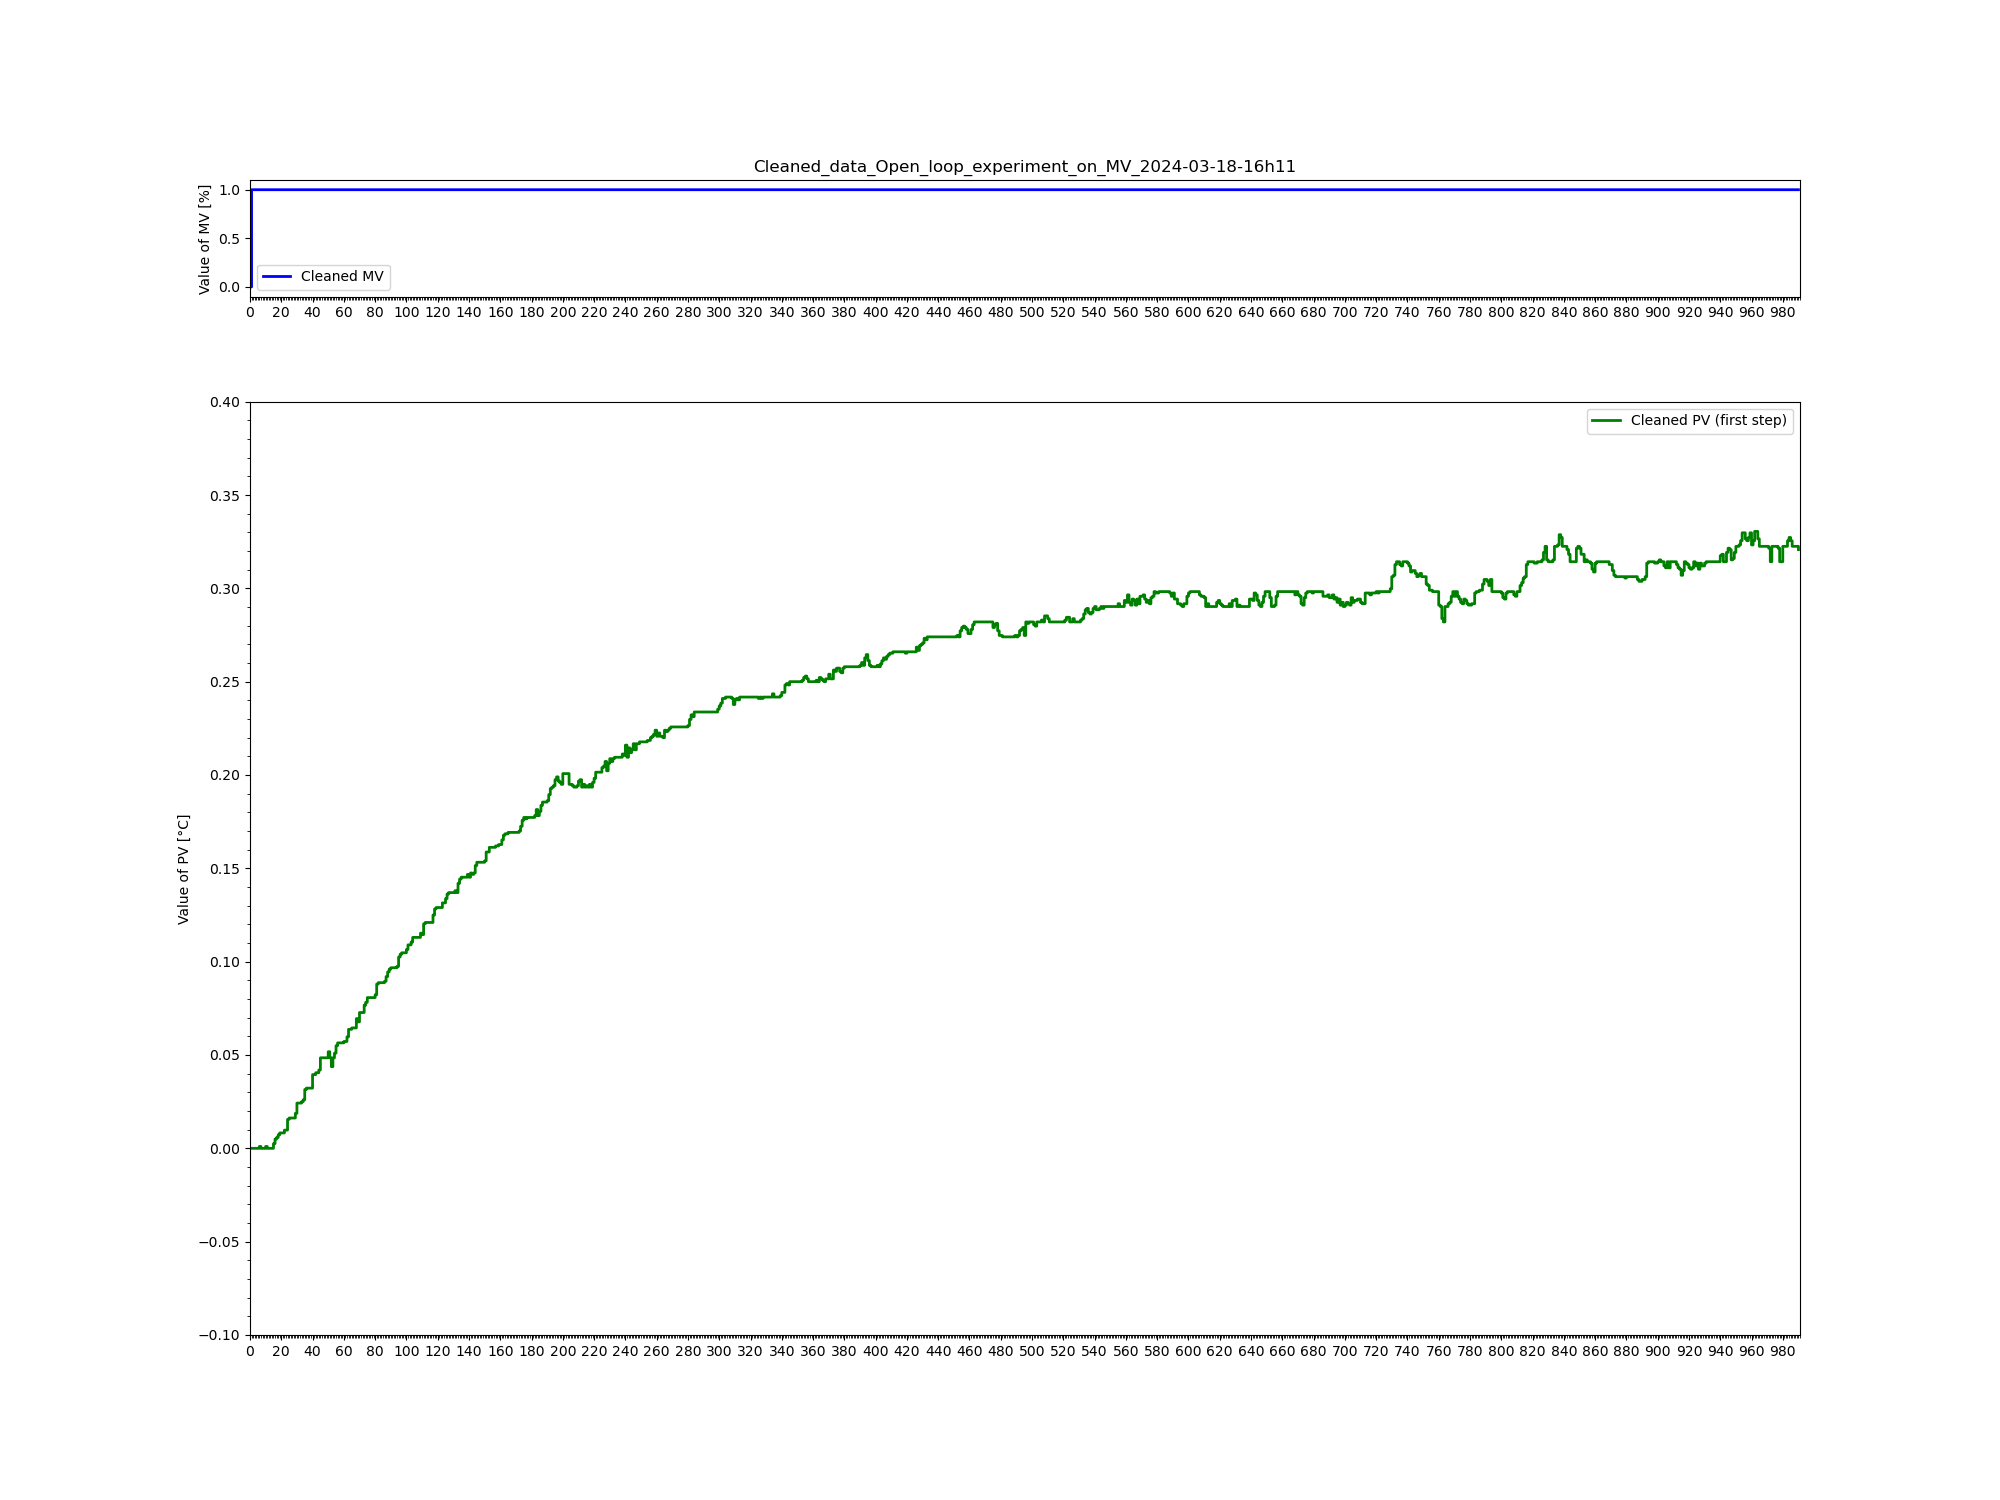
\includegraphics[width=0.9\textwidth]{../Plots/Graphical_methods_Cleaned_data_Open_loop_experiment_on_MV_2024-03-18-16h11.png}
    \caption{Réponse à un step sur MV}
    \label{fig:MV_step_response}
\end{figure}
\begin{enumerate}
    \item Le graphique (Figure \ref{fig:MV_step_response}) obtenu permet (presque) d'affirmer que le processus est un système du $1^{e}$ ordre avec un délai. L'allure de la "step response" est donc $y(t) = K_p (1-e^{-t/T})u(t)$.

    \item Le but est maintenant d'obtenir les paramètres de la fonction de transfert du processus $P(s)$ ce qui permettra de prédire $Y(s)$ pour n'importe quel $X(s)$ puisque $Y(s) = P(s) \cdot X(s)$ ou $PV = P(s)\cdot MV$. 
    \\Pour se faire, on utilise une fonction de minimisation d'erreur : 
    \begin{python*}
        minimize(FOPDT_cost,
            p0,args=(MVm,PVm,Ts,
            (fig,ax1,l1,l2)), 
            method='Powell',
            bounds=bnds,
            options={'maxiter': maxIter})
    \end{python*}

    Où \texttt{p0} contient les points de départ d'optimisation pour les paramètres \texttt{Kp, T} et \texttt{theta}. La fonction de minimisation va faire varier ces paramètres afin que la fonction de coût, \texttt{FOPDT\_cost}, renvoie la valeur la plus basse possible. 
    \\ \texttt{FOPDT\_cost} : 

    \begin{python*}
        for i in range(0,len(MV)):
            t.append(i*Ts) #calcule le temps correspondant au point actuel                  de la donnée en se basant sur la période de sample
            MVTemp.append(MV[i]) #itère sur la longueur du vecteur d'entrée

            Delay_RT(MVTemp,theta,Ts,MVDelay) #application d'un délai à MV  
            FO_RT(MVDelay,Kp,T,Ts,PVSim) #On applique un délai au premier ordre via le délai appliqué à MV puis on calcule un point du vecteur de sortie à chaque itération 
            objective = objective + (PV[i] - PVSim[i])**2 #on ajoute le carré de l'erreur actuel à la somme des carré des erreurs précédentes   
    \end{python*}
\end{enumerate}

Le fichier \texttt{Identification.ipynb} permet de trouver les valeurs estimées de $K_P$, $T_1p$, $T_2p$ et $\theta_p$ qui vont par après nous servir à modéliser le Processus et la Perturbation de façon optimale, ainsi que les différentes méthodes d'approximations des modèles du $1^{e}$ et $2^{e}$ ordre.\\
Pour notre réponse du Processus, nous obtenons les valeurs suivantes pour un modèle du $2^{e}$ ordre :
\begin{align*}
    K_P &= 0.308 \\
    T_{1p} &= 183.819 \,s \\
    T_{2p} &= 3.292 \cdot 10^{-12} \,s \\
    \theta_p &= 20.015 \,s
\end{align*}
Et les valeurs suivantes pour un modèle du $1^{er}$ ordre :
\begin{align*}
    K_P &= 0.314 \\
    T_{p} &= 206.264 \,s \\
    \theta_p &= 12.999 \,s
\end{align*}
On remarque directement que $T_{2p}$ est négligeable par rapport à $T_{1p}$, et permet donc de confirmer que le processus agit comme un système du $1^{er}$ ordre avec délai :
\begin{equation}
    \hat{P}(s) = \frac{K_P\,e^{-\theta_p s}}{(T_{1p}s + 1)(T_{2p}s + 1)} \approx \frac{K_P\,e^{-\theta_p s}}{T_{1p}s + 1}
\end{equation}

\subsubsection{Approximation graphique du modèle pour MV}

Il est également possible de déterminer la dynamique du Processus graphiquement sur base de la Figure \ref{fig:MV_step_response}.
Nous obtenons les paramètres $K_P$, $T_u$, $T_g$, $t_1$, $t_2$ et $a$ dont la détermination est expliquée en Annexe \ref{appendix:MV_graphical_method} :
\begin{align*}
    K_P &= 0.305 \\
    T_u &= 17 \,s \\
    T_g &= 211 \,s \\
    t_1 &= 95 \,s \\
    t_2 &= 133 \,s \\
    a &= 0.1
\end{align*}
Ces paramètres servirons à utiliser les méthodes classiques d'approximation du modèle, à savoir le modèle de \textbf{Broida}, \textbf{Van Der Grinten} et \textbf{Strejc}.

\subsubsection{Modèle de Broida (FOPDT)}
Ce modèle consiste à approximer le Processus par un système du $1^{er}$ ordre avec délai de la forme :
\begin{equation*}
    P_B(s) = \frac{K_P\,e^{-\theta s}}{T s + 1}
\end{equation*}
Le \underline{$1^{er}$ modèle} de Broida est obtenu en définissant la constante de temps $T$ et le délai $\theta$ comme suit :
\begin{center}
    $T = T_g = 211\,s$ \, et \, $\theta = T_u = 17\,s$
\end{center}
Le \underline{$2^{e}$ modèle} de Broida est obtenu en définissant la constante de temps $T$ et le délai $\theta$ comme suit :
\begin{center}
    $T = 5.5\,(t_2 - t_1) = 209\,s$ \, et \, $\theta = 2.8\,t_1 - 1.8\,t_2 = 26.60\,s$
\end{center}

\subsubsection{Modèle de van der Grinten (SOPDT)}
Ce modèle consiste à approximer le Processus par un système du $2^{e}$ ordre avec délai de la forme :
\begin{equation*}
    P_{vdG}(s) = \frac{K_P\,e^{-\theta s}}{(T_1 s + 1)(T_2 s + 1)}
\end{equation*}
$T_1$, $T_2$ et $\theta$ sont obtenus comme suit :
\begin{align*}
        T_1 &= T_g\,\frac{3ae - 1}{1 + ae} = -30.61\,s\\
        T_2 &= T_g\,\frac{1 - ae}{1 + ae} = 120.81\,s\\
        \theta &= T_u - \frac{T_1T_2}{T_1 + 3T_2} = 28.15\,s
\end{align*}
Nous constatons que la $1^{e}$ constante de temps $T_1$ est négative, ce qui est physiquement impossible! 
Il n'est cependant pas étonnant d'obtenir ce résultat étant donné que le Processus est un système du $1^{er}$ ordre avec délai.
Un modèle du $2^{e}$ ordre tel que van der Grinten n'est donc pas adapté pour approximer notre Processus et ne sera donc pas représenté par après.

\subsubsection{Modèle de Strejc}
Ce modèle consiste à approximer le Processus par un système du $n^{e}$ ordre avec des pôles et constantes de temps identiques de la forme :
\begin{equation*}
    P_S(s) = \frac{K_P\,e^{-\theta s}}{(T s + 1)^n}
\end{equation*}
L'ordre $n$ est obtenu avec la Table \ref{tab:Strejc_order} :
\begin{table}[H]
    \centering
    \begin{tabular}{|c|c|c|} 
        \hline
        Order $n$ & $T_{u_{th}}/T_g$ & $T_g/T$ \\
        \hline
         & $a_n$ & $b_n$ \\
        \hline
        1 & 0.00 & 1.00 \\
        \hline
        2 & 0.10 & 2.72 \\
        \hline
        3 & 0.22 & 3.69 \\
        \hline
        4 & 0.32 & 4.46 \\
        \hline
        5 & 0.41 & 5.12 \\
        \hline
        6 & 0.49 & 5.70 \\
        \hline
        7 & 0.57 & 6.23 \\
        \hline
    \end{tabular}
    \caption{Ordre $n$ du modèle de Strejc en fonction de $a_n$ et $b_n$}
    \label{tab:Strejc_order}
\end{table}
Nous avons que $T_u/T_g = 0.08$ et donc ce situe à $a_1 \leq 0.08 < a_2$, ce qui nous donne un ordre $n = 1$. $a_n$ vaut alors 0.00 et $b_n$ vaut 1.00.
La constante de temps $T$ et le délai $\theta$ vont être au final trouvés directement avec les valeurs de $T_g$ et $T_u$ comme le modèle de Broida :
\begin{align*}
    T = \frac{T_g}{b_n} = T_g = 211\,s\\
    \theta = T_u - a_n T_g = T_u = 17\,s
\end{align*}

\subsubsection{Comparaison des modèles d'approximation}

\begin{figure}[H]
    \centering
    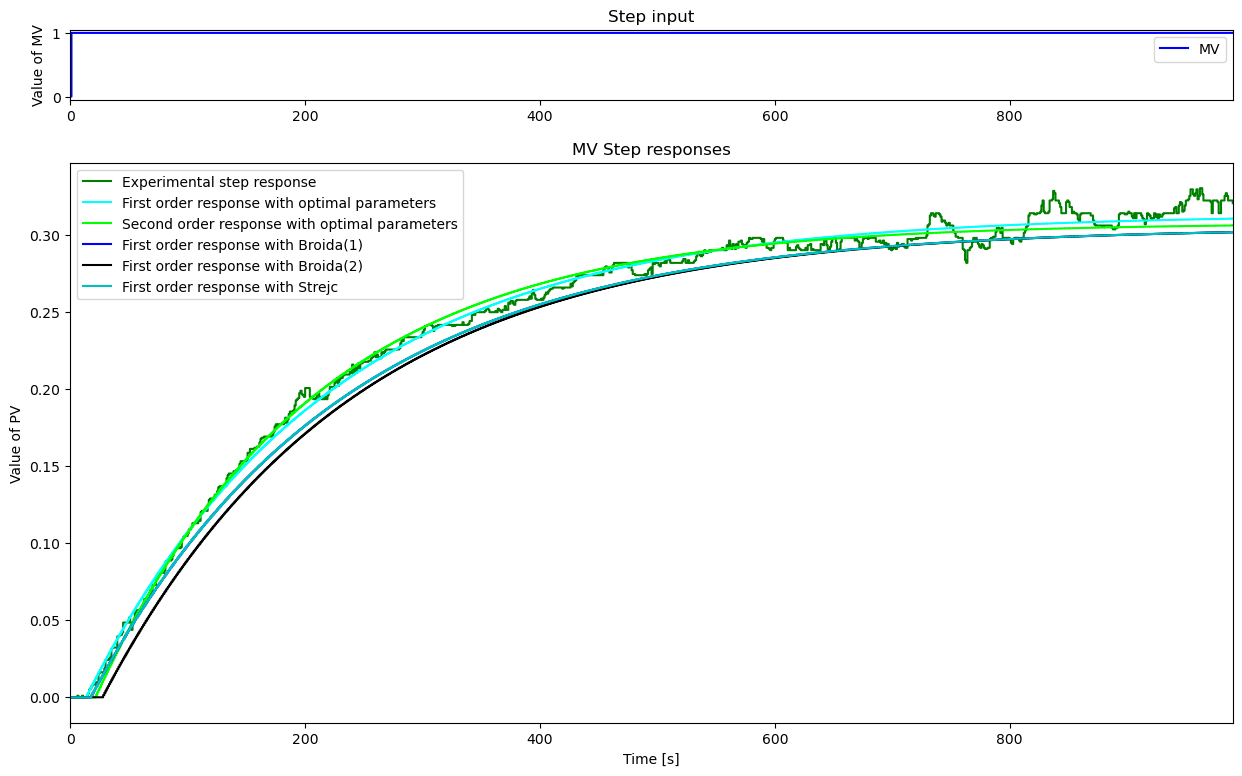
\includegraphics[width=0.9\textwidth]{../Plots/MV_Approximations_comparison_time.png}
    \caption{Approximations de la réponse temporelle d'un step sur MV}
    \label{fig:MV_approximation_comparison_time}
\end{figure}
\begin{figure}[H]
    \centering
    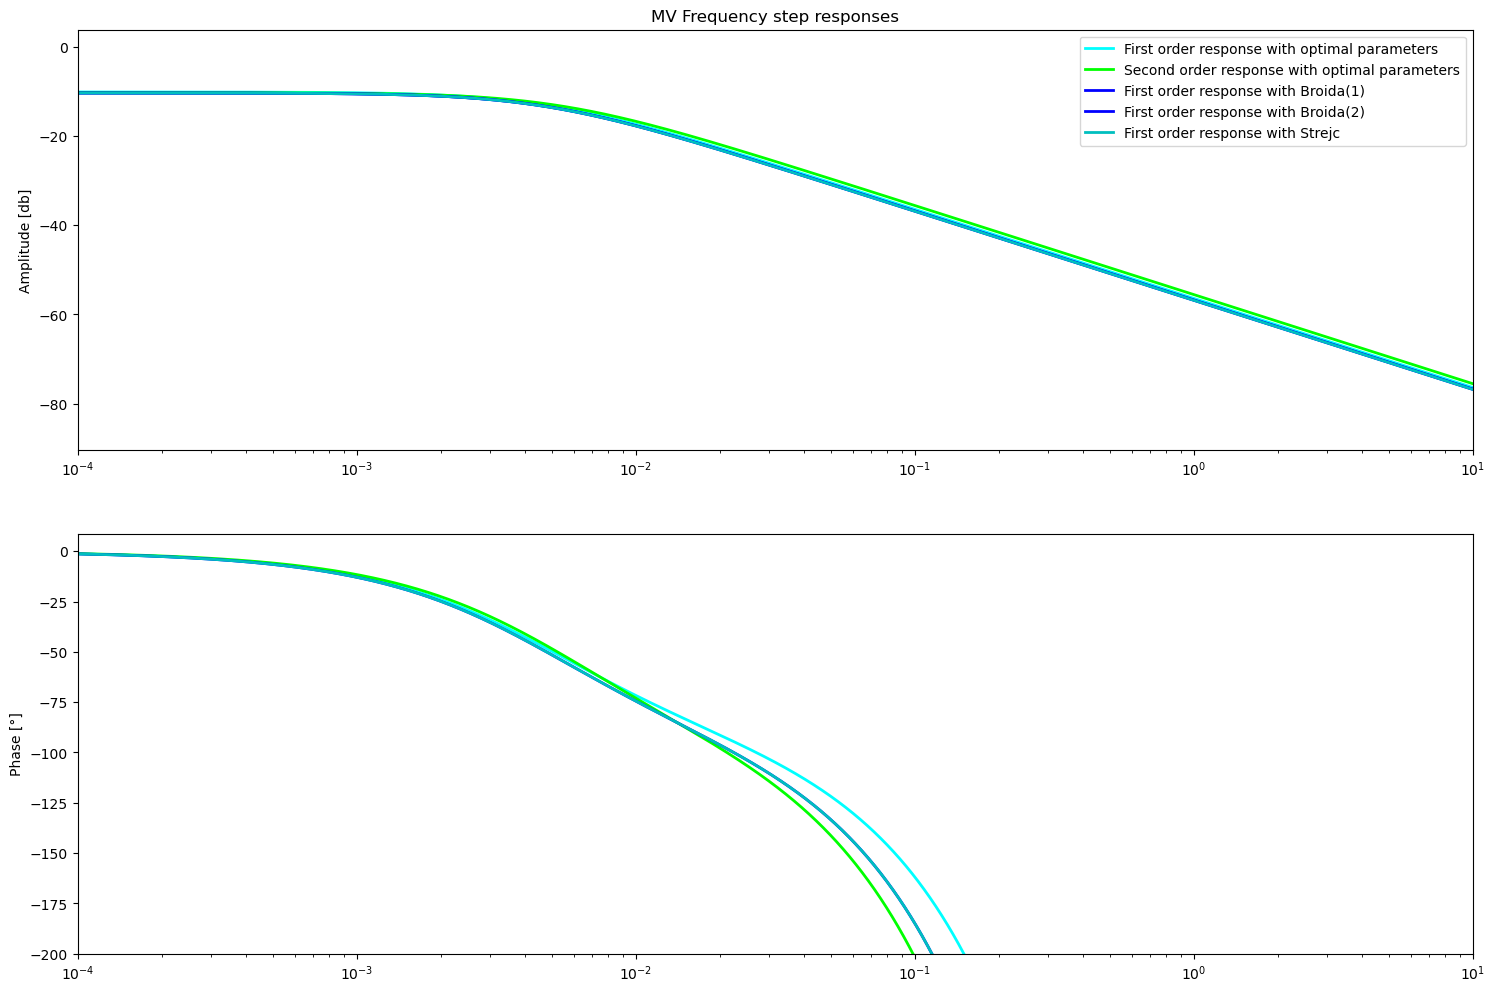
\includegraphics[width=0.9\textwidth]{../Plots/MV_Approximations_comparison_frequency.png}
    \caption{Approximations de la réponse fréquentielle d'un step sur MV}
    \label{fig:MV_approximation_comparison_frequency}
\end{figure}

La Figure \ref{fig:MV_approximation_comparison_time} montre les différentes réponses d'un step sur MV pour chacun des modèles décrits au-dessus (à l'exeption du modèle de van der Grinten).
Elles représentent toutes bien une réponse du $1^{e}$ ordre avec délai, et restent assez proches les unes des autres.
Les modèles commencent tous avec un délai similaire et terminent en régime établi à environ le même gain statique $K_P$.\\
Cependant, on distingue tout de même les modèles avec paramètres optimaux des modèles graphiques.
Les paramètres optimaux ont étés trouvés par un algorithme de minimisation de l'erreur, tandis que les paramètres graphiques ont étés trouvés par une méthode graphique dont la précision est à prendre avec recul.
\par
La Figure \ref{fig:MV_approximation_comparison_frequency} nous permet ensuite de comparer les réponses fréquentielles des différents modèles.
La première observation est que tous les modèles sont pratiquement supperposés en terme de gain.
En basses fréquences, ils atteignent bien un gain de $K_P = -10\,dB = 0.3$ et en hautes fréquences, ils subissent tous une pente de $-20\,dB$/décade.
On peut également confirmer que la réponse du $2^{e}$ ordre avec paramètres optimaux est bien en fait un $1^{er}$ ordre en raison d'une constante de temps négligeable.\\
En ce qui concerne la phase, on obtient bien une allure à la quelle on s'attendait pour un système du $1^{er}$ ordre avec délai, à savoir une phase qui tends vers l'infini (en négatif) lorsque la fréquence tends vers l'infini.
Nous constatons que la courbe bleue (premier ordre optimal) et la courbe verte (second ordre optimal) dévient plus la fréquence augmente. Cela peut être expliqué par la différence entre les deux délais $\theta_p$ qui sont de 13 et 20 secondes respectivement.
En effet, pour atteindre une même phase représenté par $\theta s = j\theta\omega$, il faudra une fréquence plus élevée pour le modèle du $1^{er}$ ordre que pour le modèle du $2^{e}$ ordre. 

%---------- Identification de la Dynamique de la Perturbation ----------%
\subsection{Perturbation D(s)}

Nous appliquons maintenant un step sur DV pour observer la réponse du système à une perturbation.
\begin{figure}[H]
    \centering
    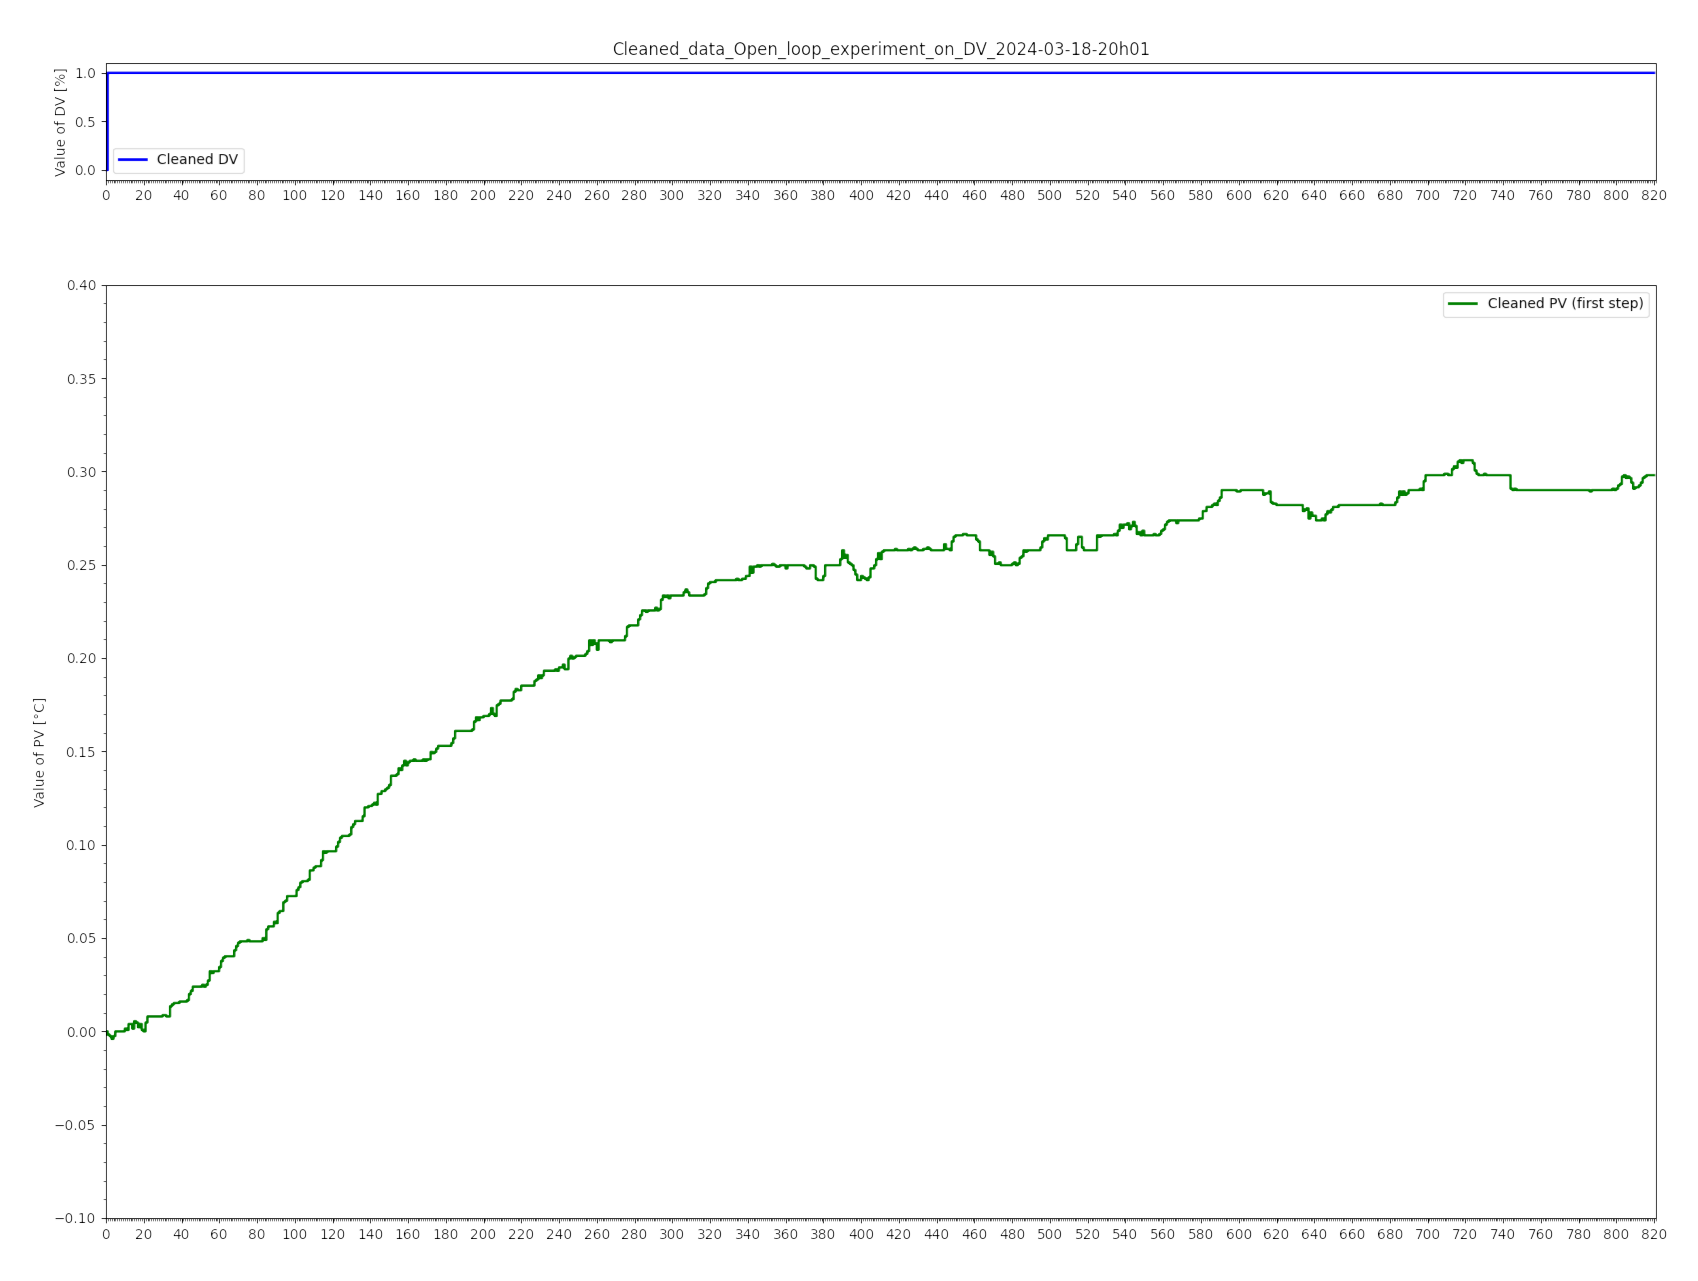
\includegraphics[width=0.9\textwidth]{../Plots/Graphical_methods_Cleaned_data_Open_loop_experiment_on_DV_2024-03-18-20h01.png}
    \caption{Réponse à un step sur DV}
    \label{fig:DV_step_response}
\end{figure}

Étant donné l'allure du graphe (Figure \ref{fig:DV_step_response}), et en particulier le point d'inflexion aux alentours de 80 secondes, nous pouvons estimer que la perturbation se comporte comme un système du $2^{e}$ ordre avec délai de la forme :
\begin{equation}
    \hat{D}(s) = \frac{K_D\,e^{-\theta_d s}}{(T_{1d}s + 1)(T_{2d}s + 1)}
\end{equation}
En effet, nous obtenons grâce au fichier \texttt{Identification.ipynb}, les valeurs optimales suivantes pour un modèle du $2^{e}$ ordre :
\begin{align*}
    K_D &= 0.295 \\
    T_{1d} &= 182.255 \,s \\
    T_{2d} &= 13.184 \,s \\
    \theta_d &= 28.999 \,s
\end{align*}
Et les valeurs suivantes pour un modèle du $1^{er}$ ordre :
\begin{align*}
    K_D &= 0.296 \\
    T_{d} &= 184.880 \,s \\
    \theta_d &= 40.136 \,s
\end{align*}
Les valeures obtenues pour $T_{1d}$ et $T_{2d}$ nous permettent de confirmer que la perturbation peut se comporter comme un système du $2^{e}$ ordre.

\subsubsection{Comparaison des modèles avec paramètres optimaux}

\begin{figure}[H]
    \centering
    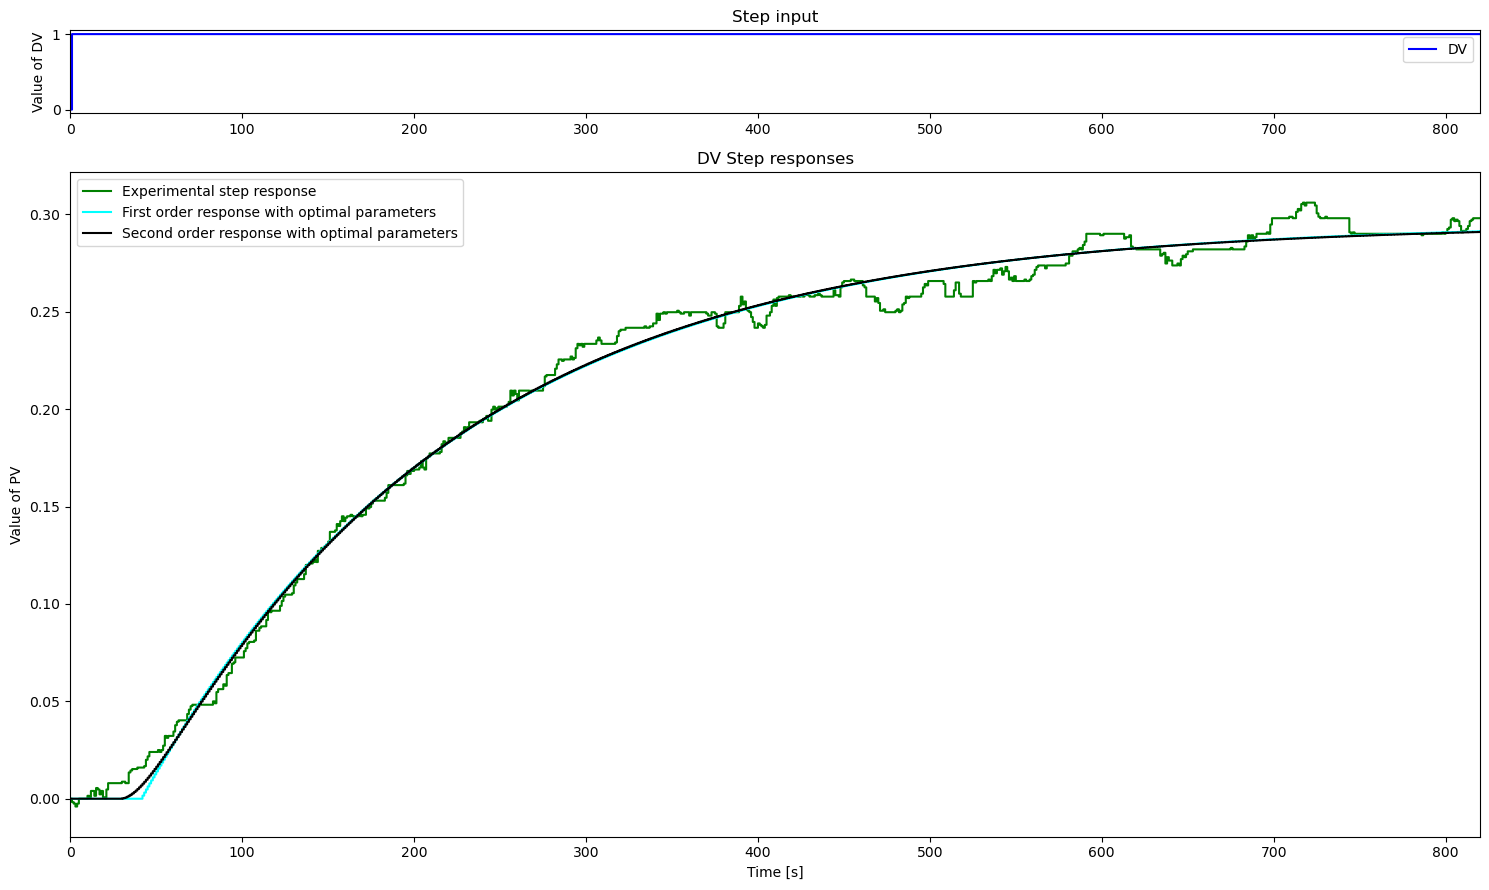
\includegraphics[width=0.9\textwidth]{../Plots/DV_Approximations_comparison_time.png}
    \caption{Approximations de la réponse temporelle d'un step sur DV}
    \label{fig:DV_approximation_comparison_time}
\end{figure}
Il est clair que la Figure \ref{fig:DV_approximation_comparison_time} montre que les modèles du $1^{er}$ et $2^{e}$ ordre avec paramètres optimaux sont très proches l'un de l'autre.
La seule différence réside en la décomposition du délai du $1^{er}$ ordre en un délai et une constante de temps $T_{2d}$ pour le $2^{e}$ ordre.
L'ajout de cette constante de temps permet de mieux modéliser la réponse expérimentale du système à une perturbation.
\begin{figure}[H]
    \centering
    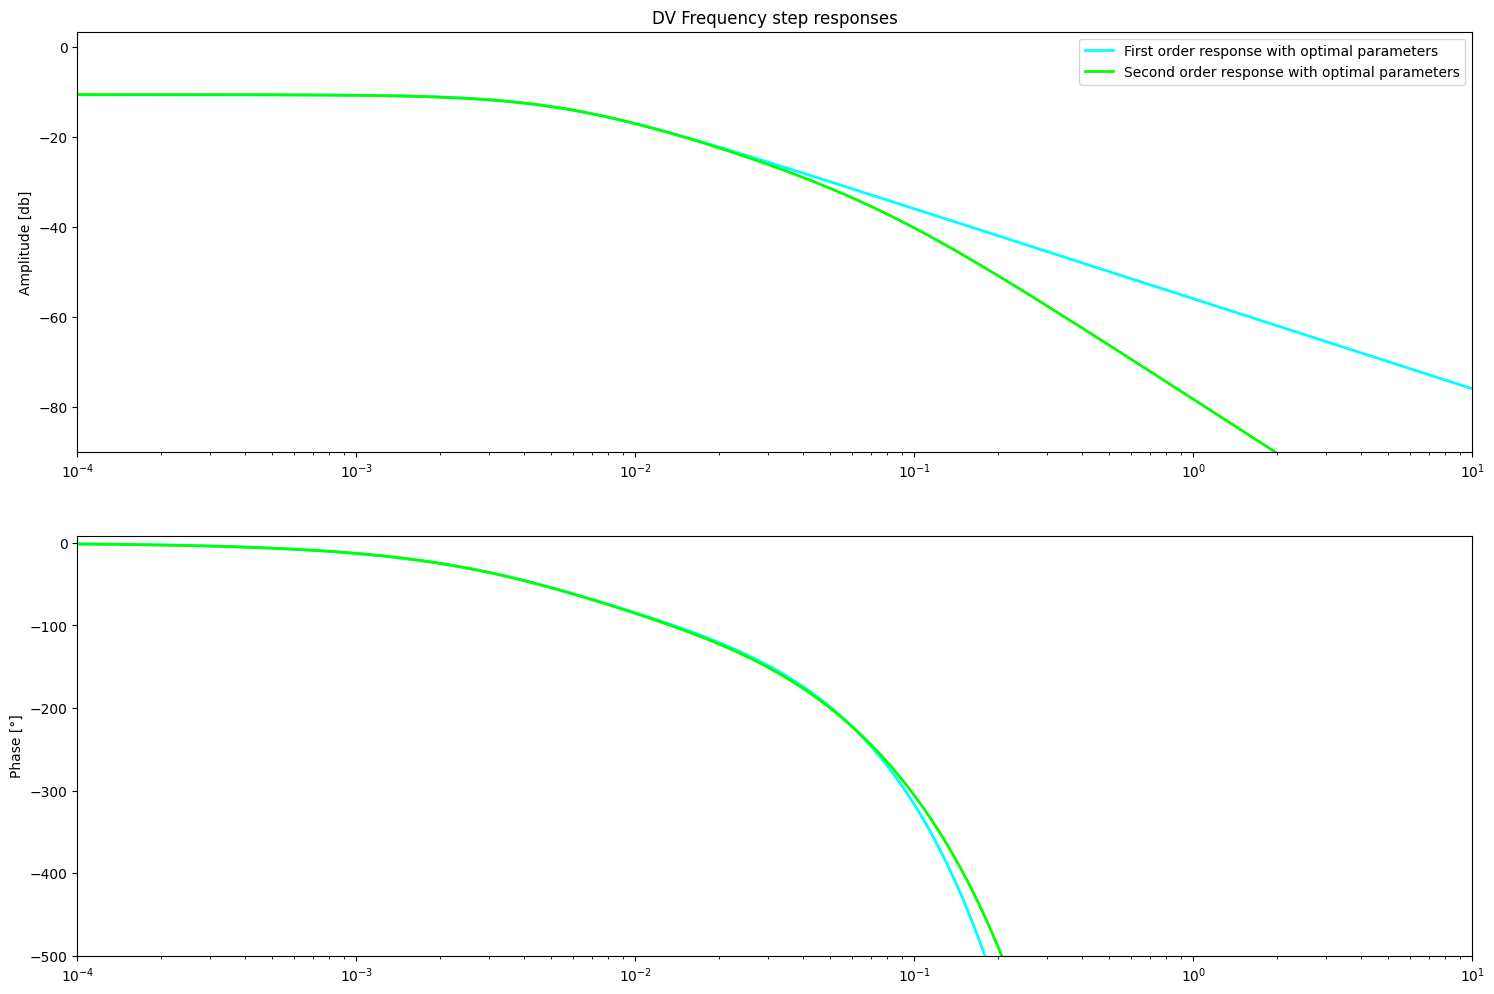
\includegraphics[width=0.9\textwidth]{../Plots/DV_Approximations_comparison_frequency.png}
    \caption{Approximations de la réponse fréquentielle d'un step sur DV}
    \label{fig:DV_approximation_comparison_frequency}
\end{figure}
Pouvant modéliser la perturbation comme un système du $1^{er}$ ou $2^{e}$ ordre avec délai, la réponse fréquentielle (Figure \ref{fig:DV_approximation_comparison_frequency}) est différente pour les deux modèles.
À hautes fréquences, le modèle du premier ordre possède une pente de $-20\,dB$/décade tandis que le modèle du second ordre possède une pente de $-40\,dB$/décade.
Le gain à basses fréquences vaut bien également $K_P = -10\,dB = 0.3$.\\
La phase, comme pour la partie Processus, tends vers l'infini (en négatif) lorsque la fréquence tends vers l'infini et dévie entre les deux modèles à hautes fréquences.
Cela peut être expliqué par la différence entre les deux délais $\theta_p$ qui sont cette fois de 40 secondes pour le premier ordre et 29 secondes pour le second ordre.
Le délai du sencond ordre étant cette fois plus petit, nous avons le comportement opposé : pour atteindre une même phase représenté par $\theta s = j\theta\omega$, il faudra une fréquence plus élevée pour le modèle du $2^{e}$ ordre que pour le modèle du $1^{er}$ ordre. 

%---------- Lead-Lag ----------%
\newpage
\section{Lead-Lag}

Un système Lead-Lag contient deux constantes de temps $T_{LEAD}$ et $T_{LAG}$, respectivement au numérateur et au dénominateur. Il peut avoir un certain gain statique $K_P$ et un délai $\theta$.
\begin{equation}
    P(s) = K_P \, \frac{T_{LEAD} s + 1}{T_{LAG} s + 1} \, e^{-\theta s}
\end{equation}
La valeur initiale du gain peut se calculer, et fait apparaître 3 scénarios : $T_{LEAD} < 0$, $T_{LEAD} > 0$ avec $T_{LEAD} > T_{LAG}$, ainsi que $T_{LEAD} > 0$ avec $T_{LEAD} < T_{LAG}$.
\begin{equation}
    y(0) = \lim_{s \to \infty} K_P \, \frac{T_{LEAD} s + 1}{T_{LAG} s + 1} \, e^{-\theta s} = K_P \, \frac{T_{LEAD}}{T_{LAG}}
\end{equation}
\begin{figure}[H]
    \centering
    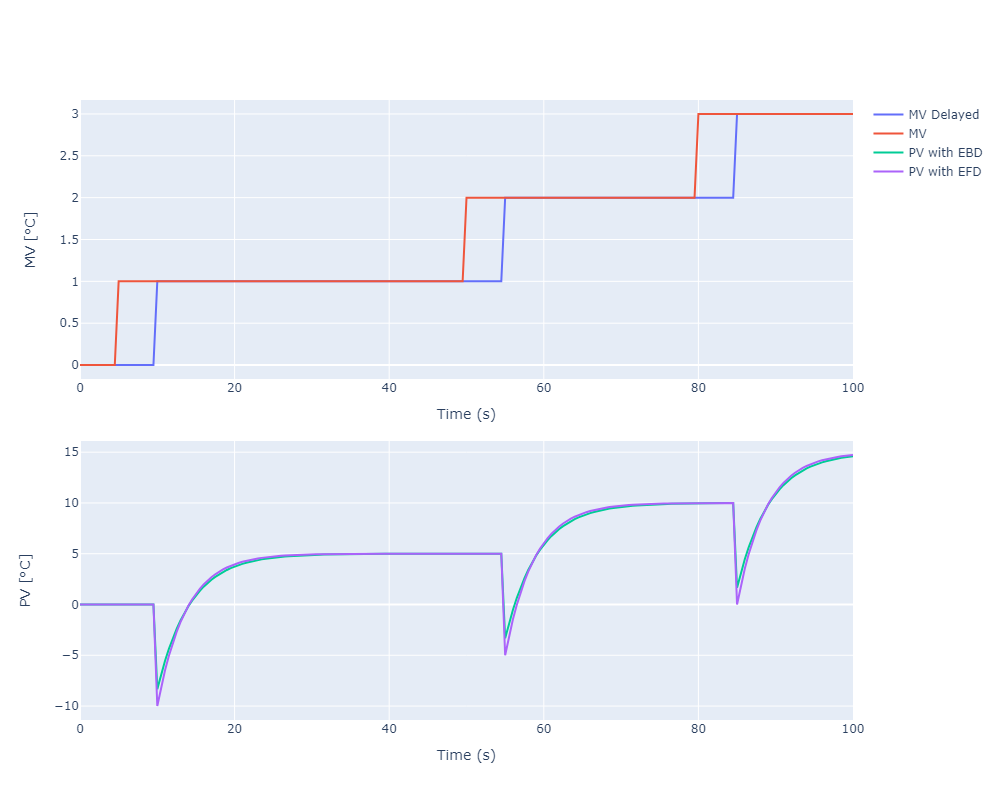
\includegraphics[width=0.8\textwidth]{../Plots/Lead-Lag/LL_Lead_negative.png}
    \caption{Réponse d'un système Lead-Lag avec $T_{LEAD} < 0$}
    \label{fig:Tlead_neg}
\end{figure}
Nous pouvons ici observer sur la Figure \ref{fig:Tlead_neg} le pic négatif dù à la constante Lead négative.
Il met ensuite un certain temps d'établissement pour atteindre le gain statique $K_P = 5$.
Le délai est également visible en voyant que $PV$ commence à agir après le délai appliqué sur $MV$.
Nous voyons de plus, que les méthodes EBD et EFD sont similaires en termes d'approximation, mais afin d'éviter les problèmes de stabilité du EFD, il est préférable d'utiliser EBD.
\begin{figure}[H]
    \centering
    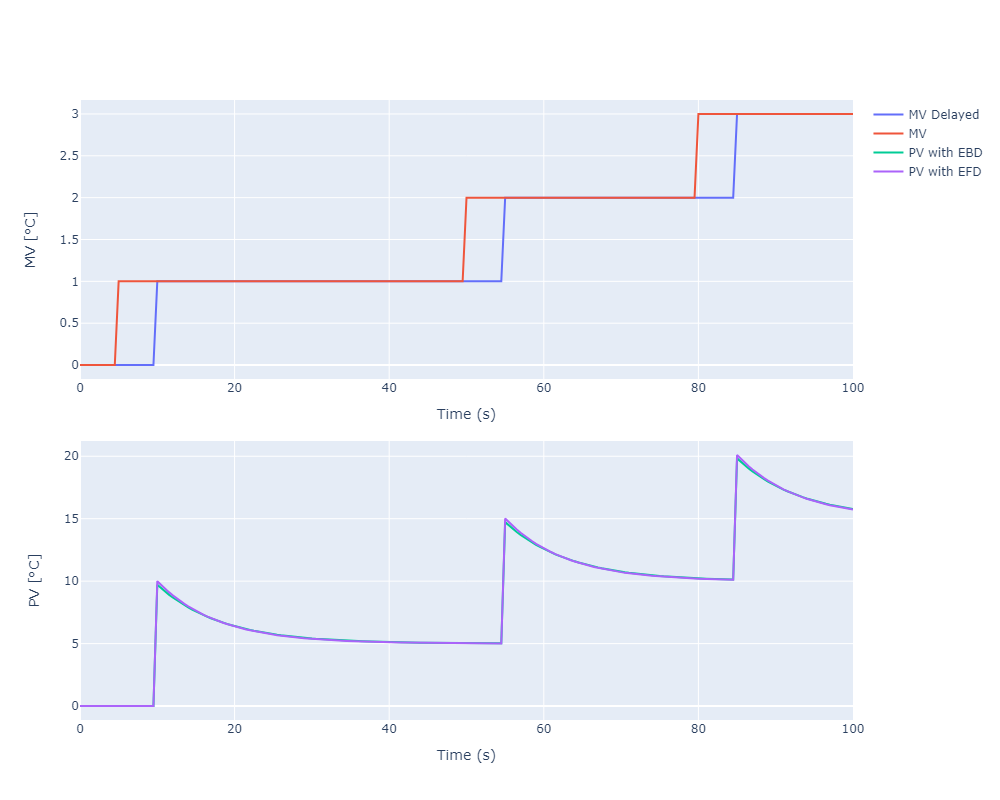
\includegraphics[width=0.8\textwidth]{../Plots/Lead-Lag/LL_Lead_higher_than_Lag.png}
    \caption{Réponse d'un système Lead-Lag avec $T_{LEAD} > T_{LAG} > 0$}
    \label{fig:Tlead_pos_Tlag_smaller}
\end{figure}
Dans le cas où $T_{LEAD} > T_{LAG}$, nous pouvons observer sur la Figure \ref{fig:Tlead_pos_Tlag_smaller} que le pic est bien positif et à une valeur double du gain statique puisque $T_{LEAD} = 2 \, T_{LAG}$.
\begin{figure}[H]
    \centering
    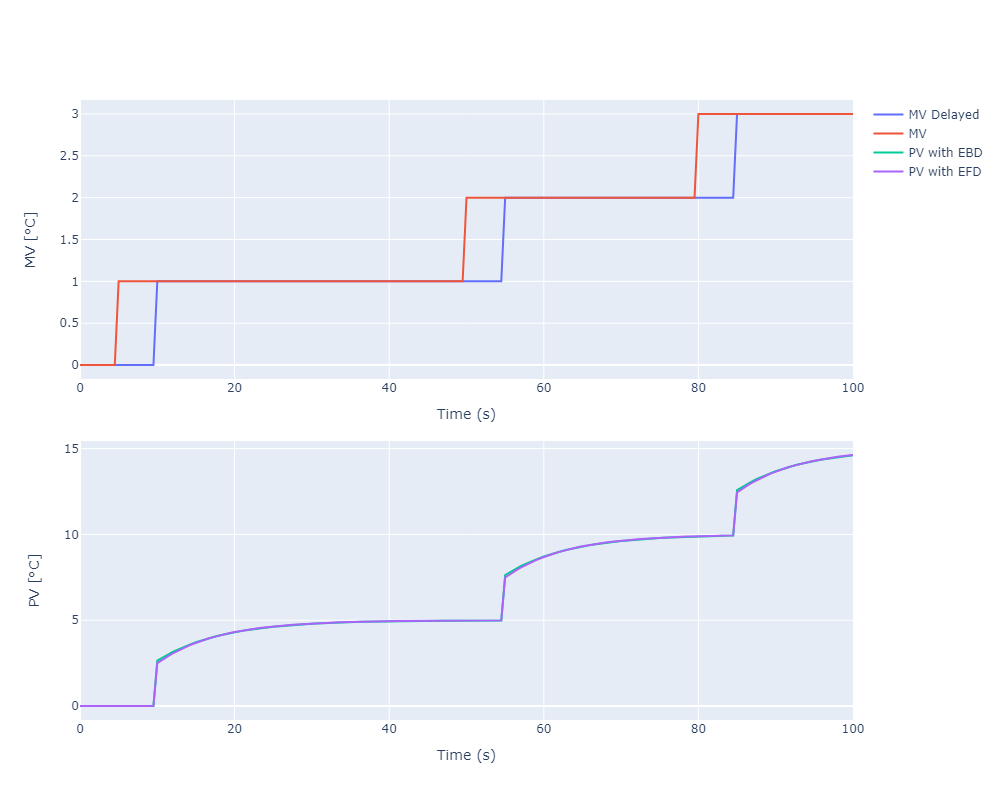
\includegraphics[width=0.8\textwidth]{../Plots/Lead-Lag/LL_Lead_lower_than_Lag.png}
    \caption{Réponse d'un système Lead-Lag avec $T_{LAG} > T_{LEAD} > 0$}
    \label{fig:Tlead_pos_Tlag_higher}
\end{figure}
Enfin, la Figure \ref{fig:Tlead_pos_Tlag_higher} montre le cas où $T_{LEAD} < T_{LAG}$, où le gain initial est 2 fois plus petit que le gain statique puisque $T_{LEAD} = 1/2 \, T_{LAG}$.

%---------- Régulateur PID ----------%
\newpage
\section{Régulateur PID}

Afin de réaliser la fonction de régulation PID avec un FeedForward, il est nécessaire de d'abord
définir les fonctions Lead-Lag (pour la partie FeedForward) et IMC Tuning (pour le calcul des constantes $K_c$, $T_i$ et $T_d$).

\subsection{FeedForward}

\begin{figure}[h]
    \centering
    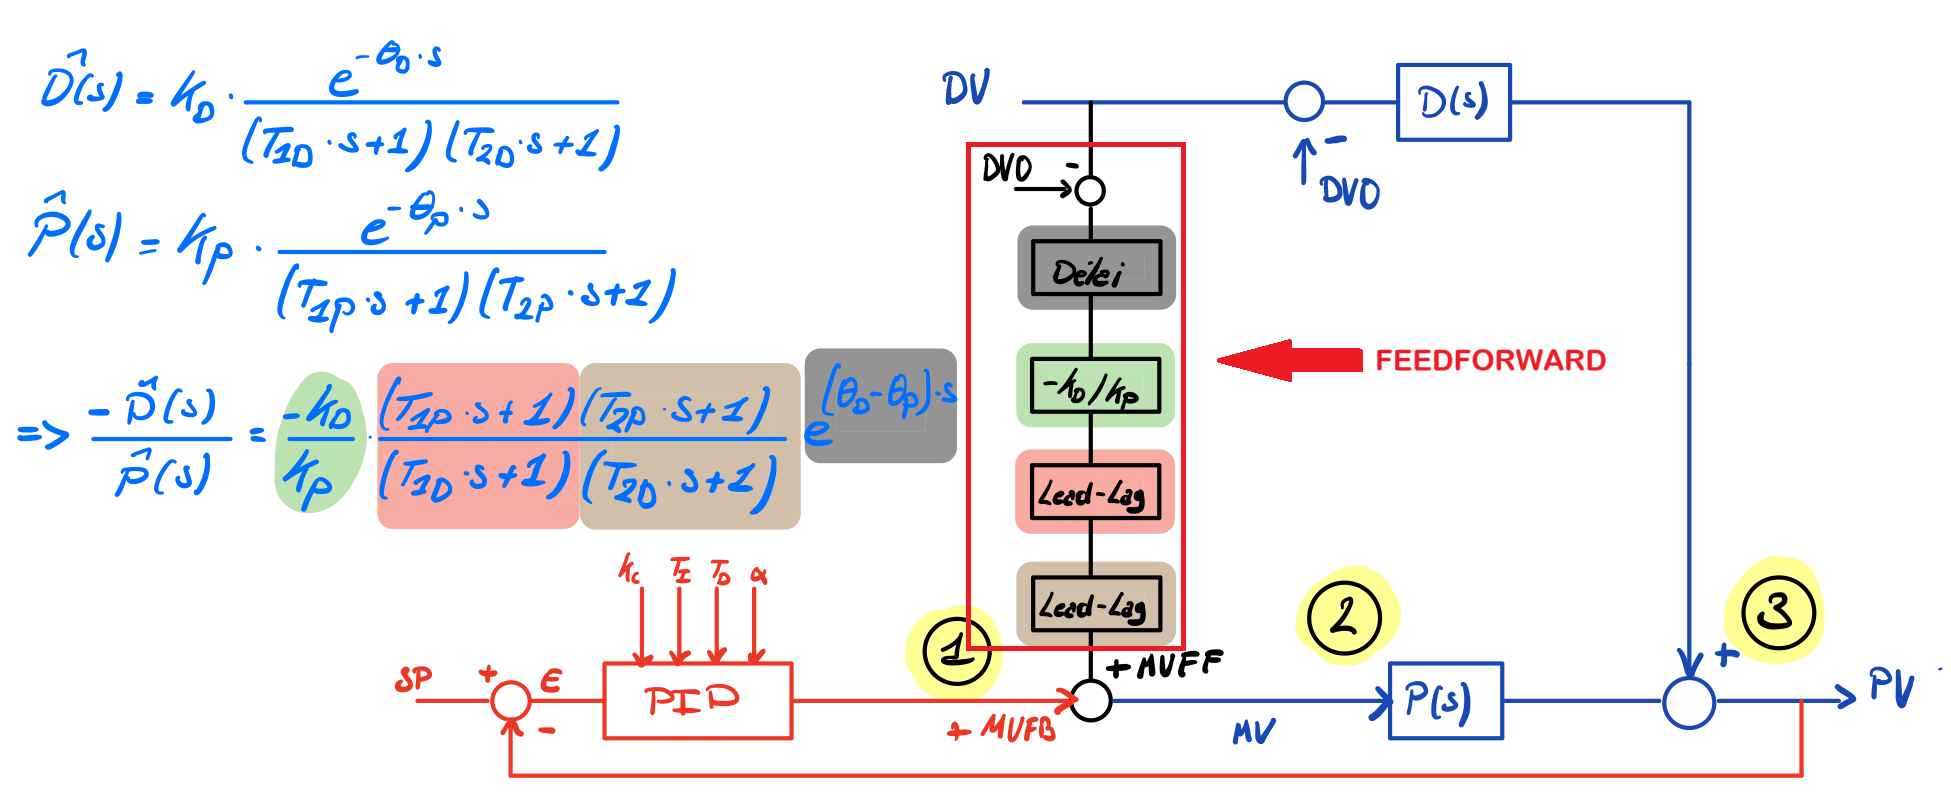
\includegraphics[width=\textwidth]{figures/schemaFF.png}
    \caption{Schema du régulateur PID avec fonction de FeedForward}
	\label{fig:schemaFF}
\end{figure}

La fonction de FeedForward est conçue pour anticiper et compenser l'impact des perturbations ($DV$) sur la variable du processus ($PV$), 
avant que ces dernières n'affectent le système.
\\Le fonctionnement du FeedForward peut être décrit de manière mathématique comme suit : 
\begin{itemize}
	\item 
	\begin{tikzpicture}
		\fill[fill=yellow!80!] (0,0) circle [radius=0.25cm];
		\node at (0,0) {1};
	\end{tikzpicture} Premièrement, la valeur manipulée en sortie du PID, $MV_{FB}$, est ajustée par une valeur $MV_{FF}$, calculée pour compenser directement la perturbation :
	\[MV_{FF} = K_{FF}\cdot\frac{(T_{1P}s + 1)(T_{2P}s + 1)}{(T_{1D}s + 1)(T_{2D}s + 1)}\cdot e^{-\theta_{FF}}\,DV = \frac{\hat{D}(s)}{\hat{P}(s)}\,DV\]
	avec : 
	\[K_{FF} = \frac{K_D}{K_P},\,\theta_{FF} = |\theta_D - \theta_P|\]
	\item 
	\begin{tikzpicture}
		\fill[fill=yellow!80!] (0,0) circle [radius=0.25cm];
		\node at (0,0) {2};
	\end{tikzpicture}Ensuite, après le n\oe{}ud $MV = MV_{FB} + MV_{FF}$, on obtient : 
	\[P(s)\cdot MV \approx P(s)\cdot MV_{FB} - \hat{D}(s)\]
	\item
	\begin{tikzpicture}
		\fill[fill=yellow!80!] (0,0) circle [radius=0.25cm];
		\node at (0,0) {3};
	\end{tikzpicture} Pour enfin arriver au n\oe{}ud final où l'on additionne la dynamique de la perturbation à celle du processus : 
	\[P(s)\cdot MV_{FB} - \hat{D}(s) + D(s) \approx P(s)\cdot MV_{FB} = PV\]
\end{itemize}
\subsubsection{Délai}

La $1^{ère}$ étape dans la réalisation de la fonction du ``FeedForward'' est de récupérer la perturbation $DV$, de la ramener au point de fonctionnement et de lui appliquer un délai $\theta_{FF} = |\theta_D-\theta_P|$ qui provient du rapport entre la dynamique de la perturbation
$\hat{D}(s)$ et du processus $\hat{P}(s)$.
Pour se faire, on utilisera la fonction \texttt{Delay\_RT} sur le signal $DV$ recentré via : 
\begin{python*}
	Delay_RT(self.DV - self.DV0*np.ones_like(self.DV), # On centre DV sur le point de fonctionnement
		max(self.theta_ODV_SOPDT-self.theta_OMV_SOPDT, 0), # Calcul du délai 
		self.Ts, 
		self.MVFF_Delay)
\end{python*}

\subsubsection{Gain et Lead-Lag}
Une fois que le délai et la translation appliqués, il faut maintenant passer au gain et au premier Lead-Lag.
\\Le gain est simplement le rapport du gain de la fonction de transfert décrivant la dynamique de perturbation et celle décrivant la dynamique de processus $K_{FF} = \frac{K_D}{K_P}$ (la raison du signe négatif sera expliquée plus tard dans le rapport).
\\Le premier Lead-Lag dont $T_{Lead} = T_{1D}$ et $T_{Lag} = T_{1P}$ couplé au gain et au délai permet d'obtenir la fonction de transfert : 
\[K_{FF}\cdot\frac{T_{1D}s + 1}{T_{1P}s + 1} \cdot e^{\theta_{FF}}\]
Pour se faire, on utilise la fonction \texttt{LL\_RT} sur le signal $DV$ retardé et centré ($MV\_Delay$) via : 
\begin{python*}
	LL_RT(self.MVFF_Delay, 
	-self.Kp_ODV_SOPDT/self.Kp_OMV_SOPDT, # gain
	self.T1_OMV_SOPDT, 
	self.T1_ODV_SOPDT, 
	self.Ts, 
	self.MVFF_LL1)
\end{python*}

\subsection{Introduction}
Afin de réguler les variations en sortie $PV$, on utilise un régulateur PID, qui reprend la valeur de $PV$ pour la soustraire à la consigne $SP$ donnant donc l'erreur $E = SP - PV$ à corriger sur $MV$.\\
Pour rappel, un régulateur PID est composé de trois termes:
\begin{itemize}
    \item Le terme proportionnel $P$ qui est proportionnel à l'erreur $E$ et vise une erreur statique nulle.
    \item Le terme intégral $I$ qui est proportionnel à la somme des erreurs passées et donc accumule l'erreur.
    \item Le terme dérivé $D$ qui est proportionnel à la dérivée de l'erreur et vise à corriger anticipativement l'erreur future.
\end{itemize}
La sortie du régulateur est alors donnée par :
\begin{equation}
    MV = K_C \, \left( 1 + \frac{1}{T_I s} + \frac{T_D s}{\alpha T_D s + 1}\right) \, E
\end{equation}

Dans le cadre du laboratoire, le régulateur utilise également le \textbf{Reset de l'Action Intégrale} et la \textbf{Saturation de l'Action Intégrale} venant adapter l'action intégrale en fonction de, respectivement, la valeur de $MV$ en mode manuel, et la saturation de $MV$ atteignant les limites $MV_{MAX}$ / $MV_{MIN}$.
\begin{center}
    $MV_I = MV_{Man} - MV_P - MV_D - MV_{FF}$\\[4pt]
    et\\[4pt]
    $MV_I = MV_{MAX} - MV_P - MV_D - MV_{FF}$
\end{center}

\subsection{Optimisation par la méthode IMC}
Il est important de choisir les paramètres $K_C$, $T_I$ et $T_D$ de façon à implémenter le bon régulateur pour notre processus.
Une façon d'obtenir ces paramètres optimaux est de réaliser un step sur $MV$ et d'observer la dynamique du Processus.
Le modèle trouvé va nous permettre de calculer ces valeurs via des tables.\\
On utilisera la ligne I du tableau présent dans le cours, correspondant à un modèle du second ordre avec délai ($\tau_3 = 0$).
\begin{align*}
    K_C &= \frac{1}{K_P} \, \frac{T_{1p} + T_{2p}}{T_{CLP} + \theta}\\[4pt]
    T_I &= T_{1p} + T_{2p}\\[4pt]
    T_D &= \frac{T_{1p} \, T_{2p}}{T_{1p} + T_{2p}}
\end{align*}
Il est bon de noter que nous aurions pu utiliser la ligne G du tableau (premier ordre avec délai) totalement équivalente étant donné que notre Processus est du premier ordre ($T_{2p} \approx 0$).
\begin{align*}
    K_C &= \frac{1}{K_P} \, \frac{T_{1p}}{T_{CLP} + \theta}\\[4pt]
    T_I &= T_{1p}\\[4pt]
    T_D &= 0
\end{align*}
La constante de temps en boucle fermée $T_{CLP}$ est un certain ratio de la première constante de temps du processus $T_{1p}$ définit par $T_{CLP} = \gamma \, T_{1p}$. L'influence de $\gamma$ sera discuté en simulation de boucle fermée par après.

\subsection{Réponse indicielle du régulateur PID}

Nous allons maintenant analyser la réponse du régulateur lorsqu'on applique une erreur $E$ constante à son entrée.
\begin{figure}[H]
    \centering
    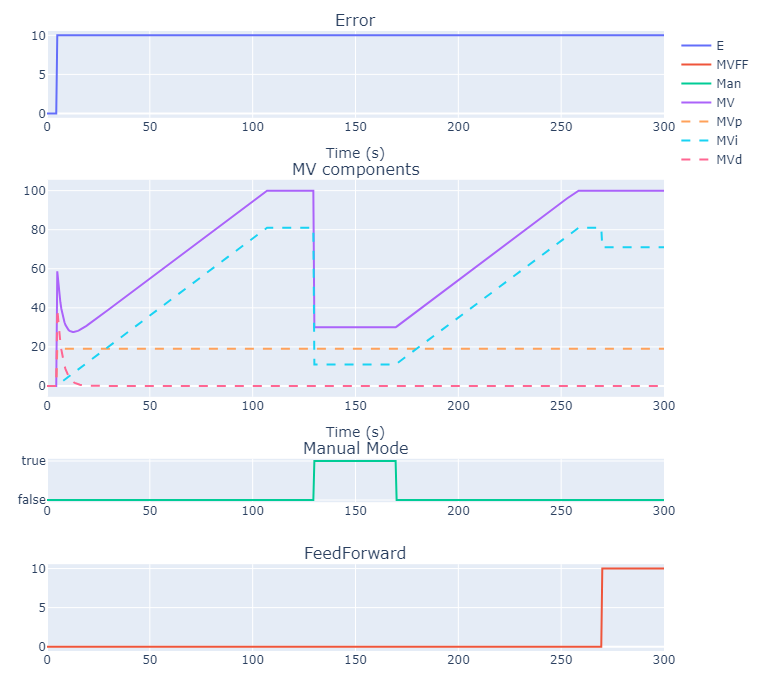
\includegraphics[width=0.9\textwidth]{../Plots/PID/PID_Response_error_step.png}
    \caption{Réponse indicielle du PID à un step sur E}
    \label{fig:Step_Response_PID}
\end{figure}



%---------- Simulation ----------%
\newpage
\section{Simulation du système}

Nous nous intéresserons maintenant au système complet afin de simuler les différentes réponses aux évènements tels que step sur $DV$, step sur $SP$ ou activation du feedforward, et ce, dans les conditions réelles des futures réponses expérimentales.

Il est bon de rappeler que tout ce qui va être simulé sera fait autour d'un point de fonctionnement, et valable uniquement aux alentours de ce point.
Dans notre cas, nous avons la puissance de chauffe du premier radiateur $MV_0 = 50\%$, la puissance de chauffe du deuxième radiateur $DV_0 = 50\%$ et la sortie du système en régime permanent $PV_0 = 49.3^{\circ}$C.

Pour l'instant, le paramètre $\alpha$ sera fixé à $\alpha = 1$ par simplicité et $\gamma$ sera fixé à $\gamma = 0.7$ pour éviter une réponse du régulateur trop aggressive.
On utilisera les paramètres optimaux du second ordre trouvés à la Section 2 \textit{Identification de la Dynamique} pour simuler le Processus et la Perturbation.

\noindent Nous alons ici analyser les scénarios suivants :
\begin{enumerate}
    \item Réponse en mode \underline{manuel} (boucle ouverte) \underline{sans} FeedForward
    \item Réponse en mode \underline{manuel} (boucle ouverte) \underline{avec} FeedForward
    \item Réponse en mode \underline{automatique} (boucle fermée) \underline{sans} FeedForward
    \item Réponse en mode \underline{automatique} (boucle fermée) \underline{avec} FeedForward
\end{enumerate}

\subsection{Réponse à une perturbation \texorpdfstring{$DV$}{DV} en mode manuel sans FF}
\begin{figure}[H]
    \centering
    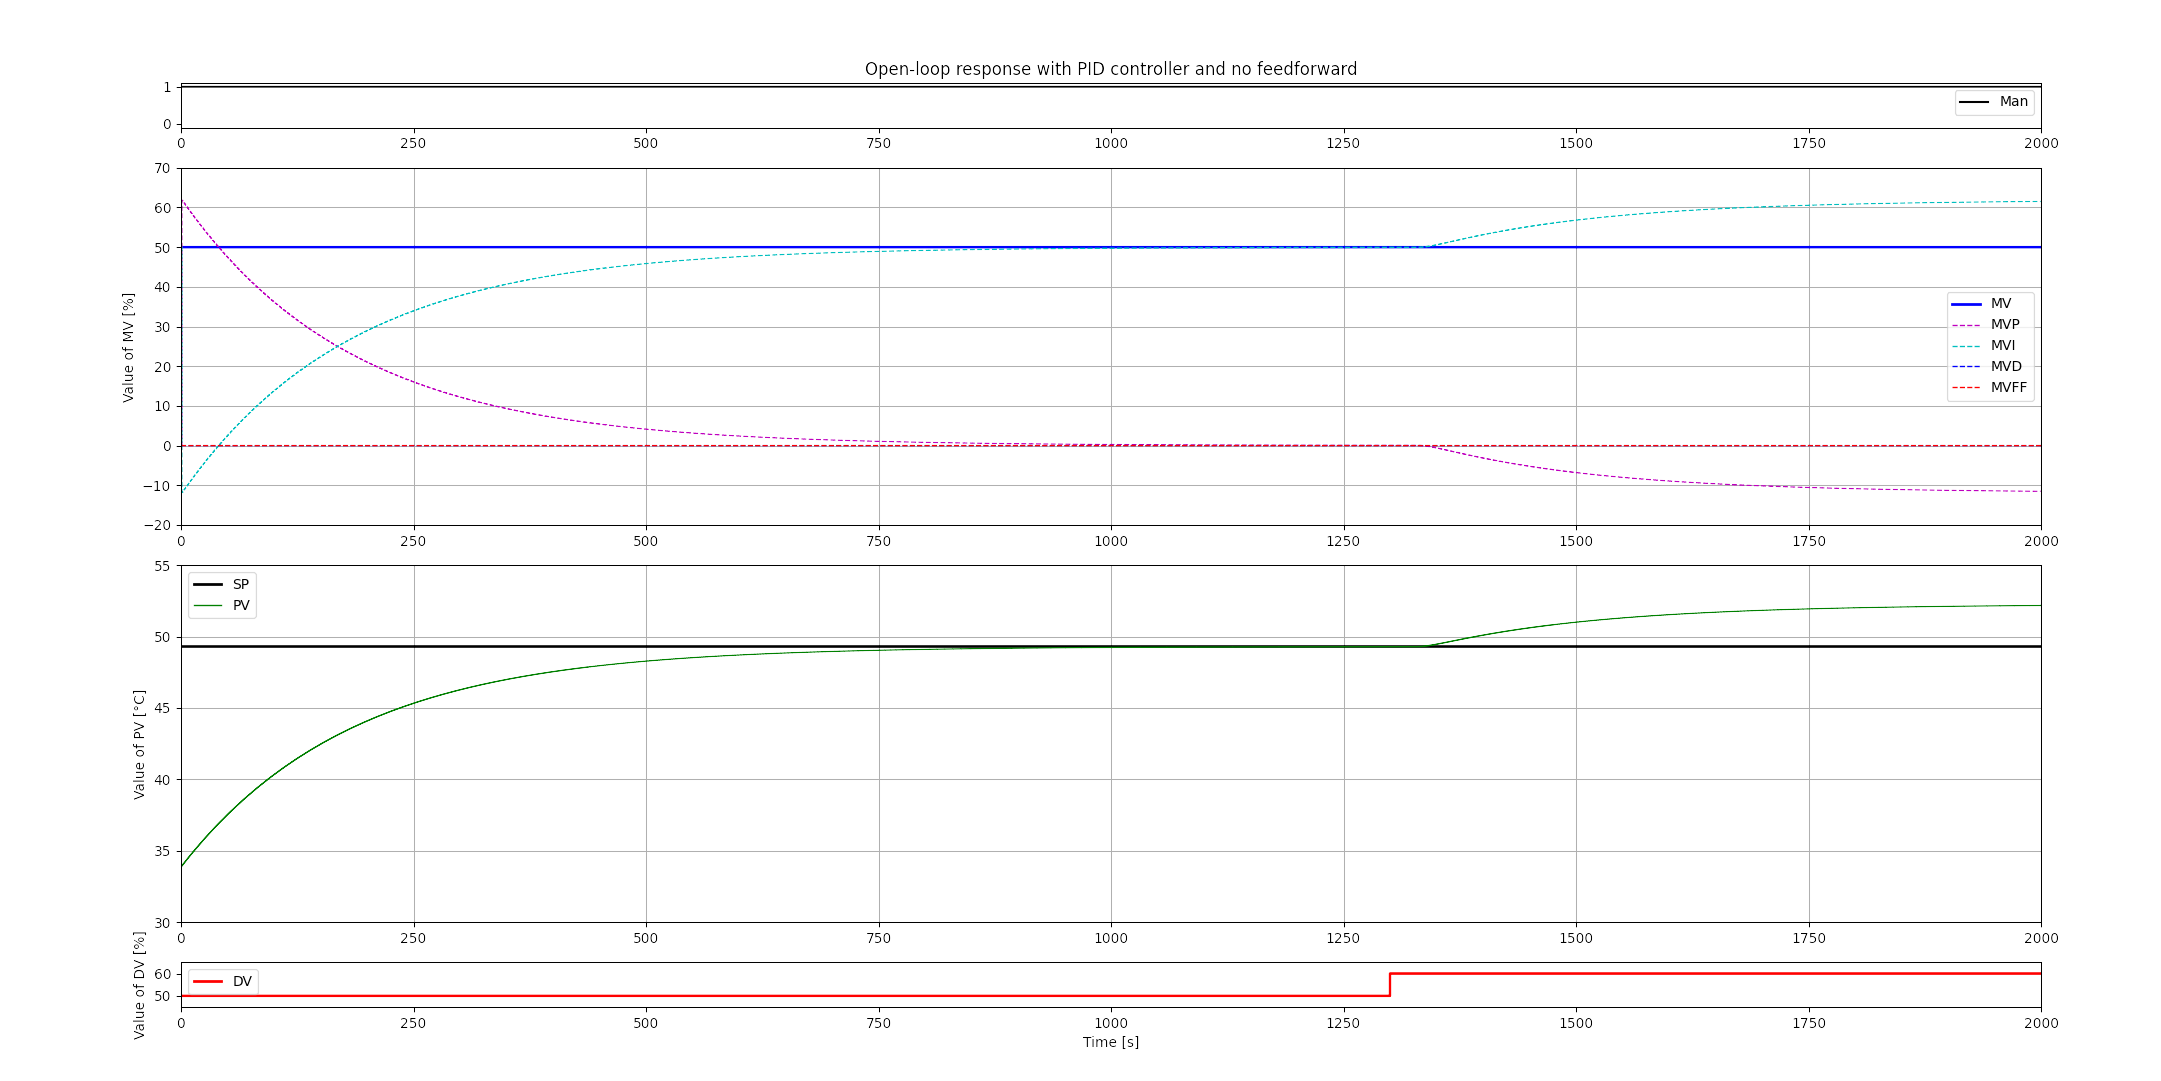
\includegraphics[width=0.9\textwidth]{../Plots/Simulation_scenario_2.png}
    \caption{Réponse à boucle ouverte sans FeedForward}
    \label{fig:Simulation_OLP_no_FF}
\end{figure}
La Figure \ref{fig:Simulation_OLP_no_FF} confirme bien que l'on est en mode manuel en imposant une valeur de $MV = MV_0$.
Il est dès lors logique de voir l'action intégrale $MV_I$ s'adapter tout le long de la simulation en raison du Reset de l'Action Intégrale.\\
Nous constatons que l'action dérivée $MV_D$ est nulle, ce qui est normal étant donné que la constante de temps $T_D$ est nulle. Notre processus agit comme un premier ordre et donc notre régulateur est assimilé à un régulateur PI.

L'action proportionnelle $MV_P$ fait un pic au début de la simulation. Cela est dû à la différence entre la consigne et la sortie du système, donc l'erreur.
En effet, la composante proportionnelle est directement proportionnelle à l'erreur et au gain statique : $MV_P = K_C \, E \approx 4 \cdot 15\% = 60\%$.\\
La sortie de processus $PV$ met alors un certain temps à se stabiliser autour de la valeur de consigne $SP = PV_0$ (temps d'établissement).

Une perturbation est alors appliquée. Le feedforward étant désactivé, elle se trouve répercutée sur $PV$.
Comme attendu, cette variation introduit une erreur négative que l'on voit sur $MV_P$. Le reset de l'action intégrale fait son travail en venant augmenter $MV_I$ afin de conserver la valeur manuelle de $MV$.\\
Il est également intéressant de retrouver le délai en regardant la différence entre le moment où la perturbation est appliquée et le moment où $PV$ réagit.

\subsection{Réponse à une perturbation \texorpdfstring{$DV$}{DV} en mode manuel avec FF}
\begin{figure}[H]
    \centering
    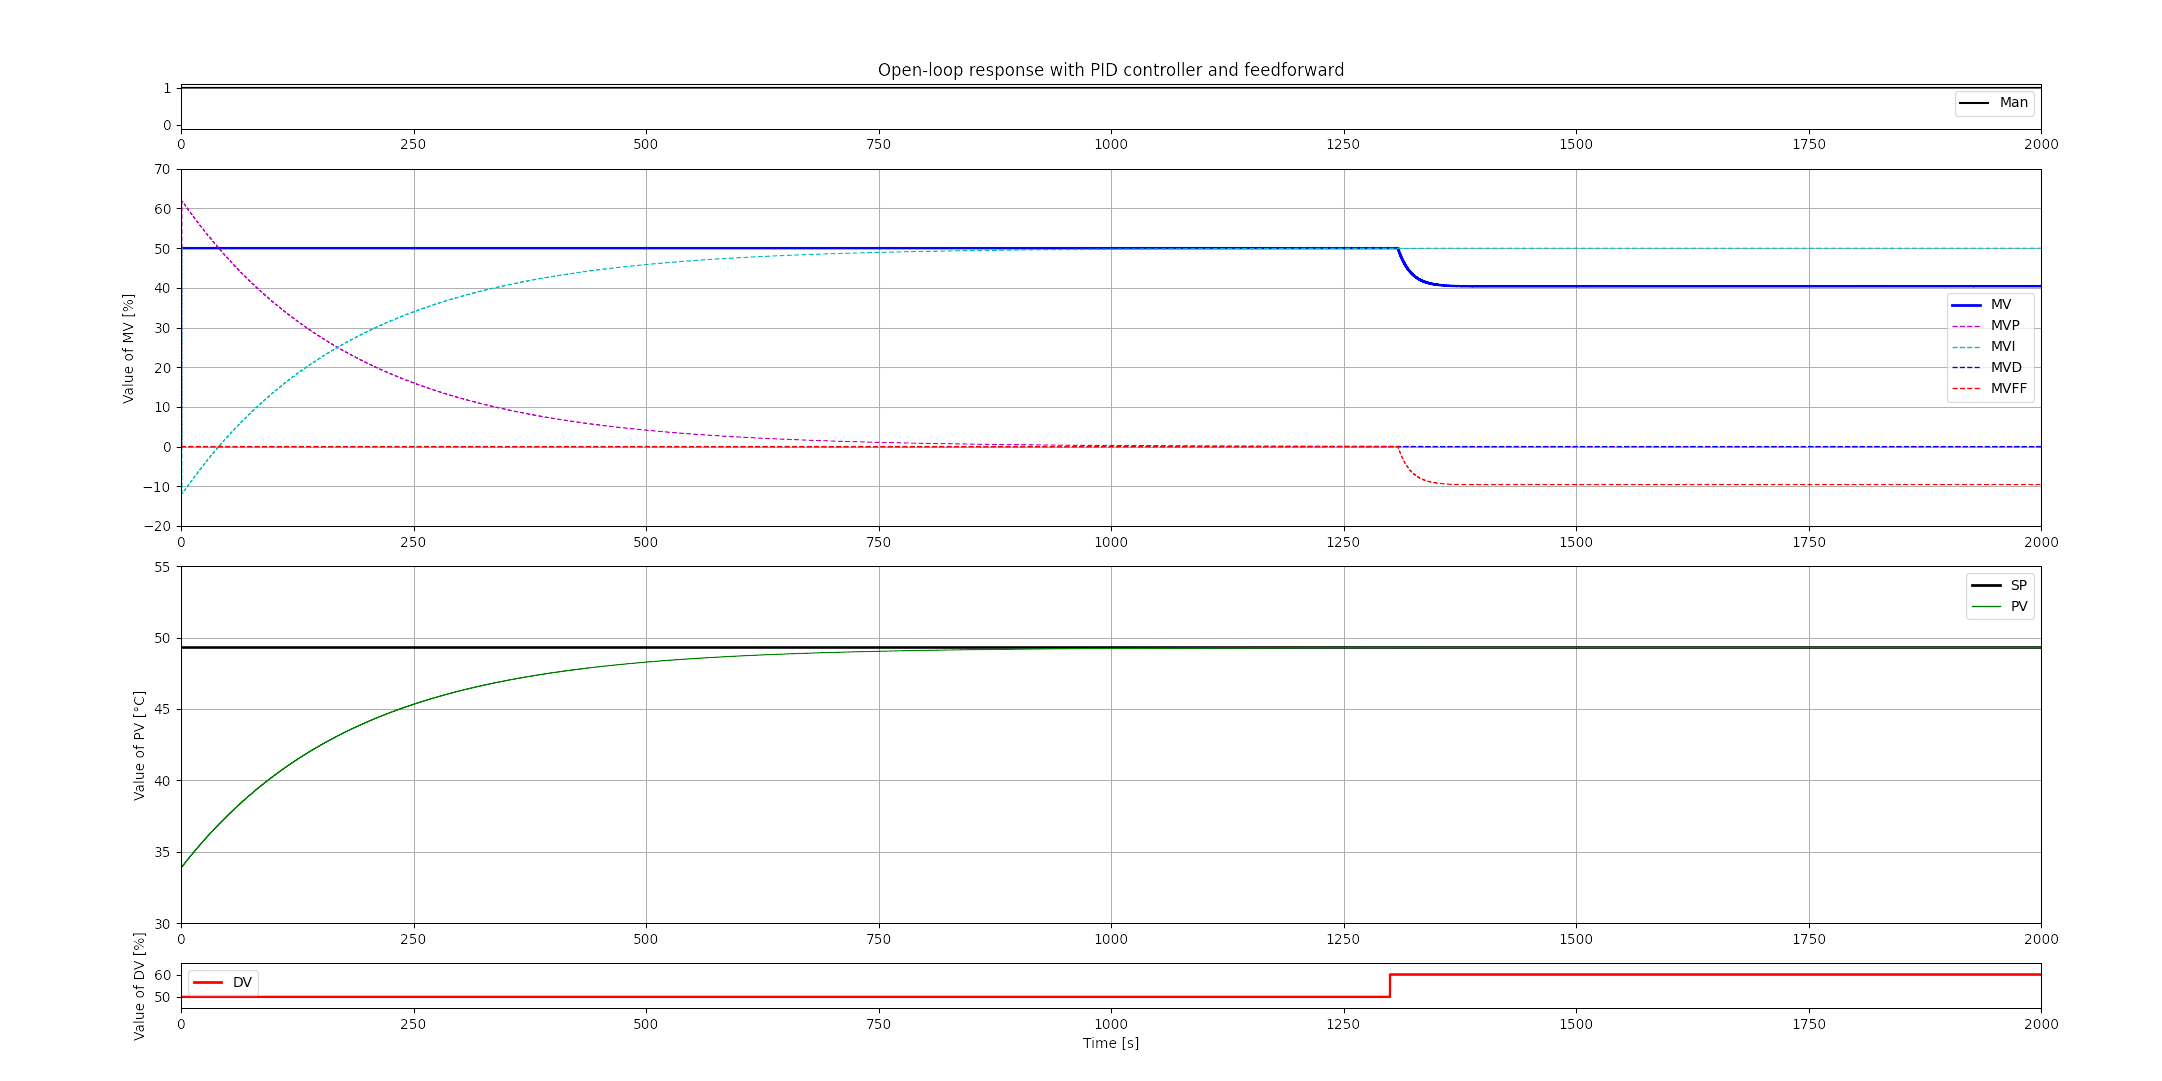
\includegraphics[width=0.9\textwidth]{../Plots/Simulation_scenario_3.png}
    \caption{Réponse à boucle ouverte avec FeedForward}
    \label{fig:Simulation_OLP_FF}
\end{figure}
Dans ce scénario, le feedforward est activé. La perturbation $DV$ est donc prise en compte anticipativement.
Nous constatons que la composante $MV_{FF}$ réagit bien comme attendu à la perturbation. $MV$ est donc lui même ajusté pour compenser la perturbation et ainsi conserver $PV = SP = PV_0$.\\
Encore une fois, nous pouvons nous intéresser au délai qui se trouve maintenant réduit puisqu'il s'agit du délai du feedforward $\theta_{FF} = \theta_D - \theta_P = 29 - 20 = 9\,s$.

\subsection{Réponse à une perturbation \texorpdfstring{$DV$}{DV} \& changement de consigne \texorpdfstring{$SP$}{SP} en mode automatique sans FF}
\begin{figure}[H]
    \centering
    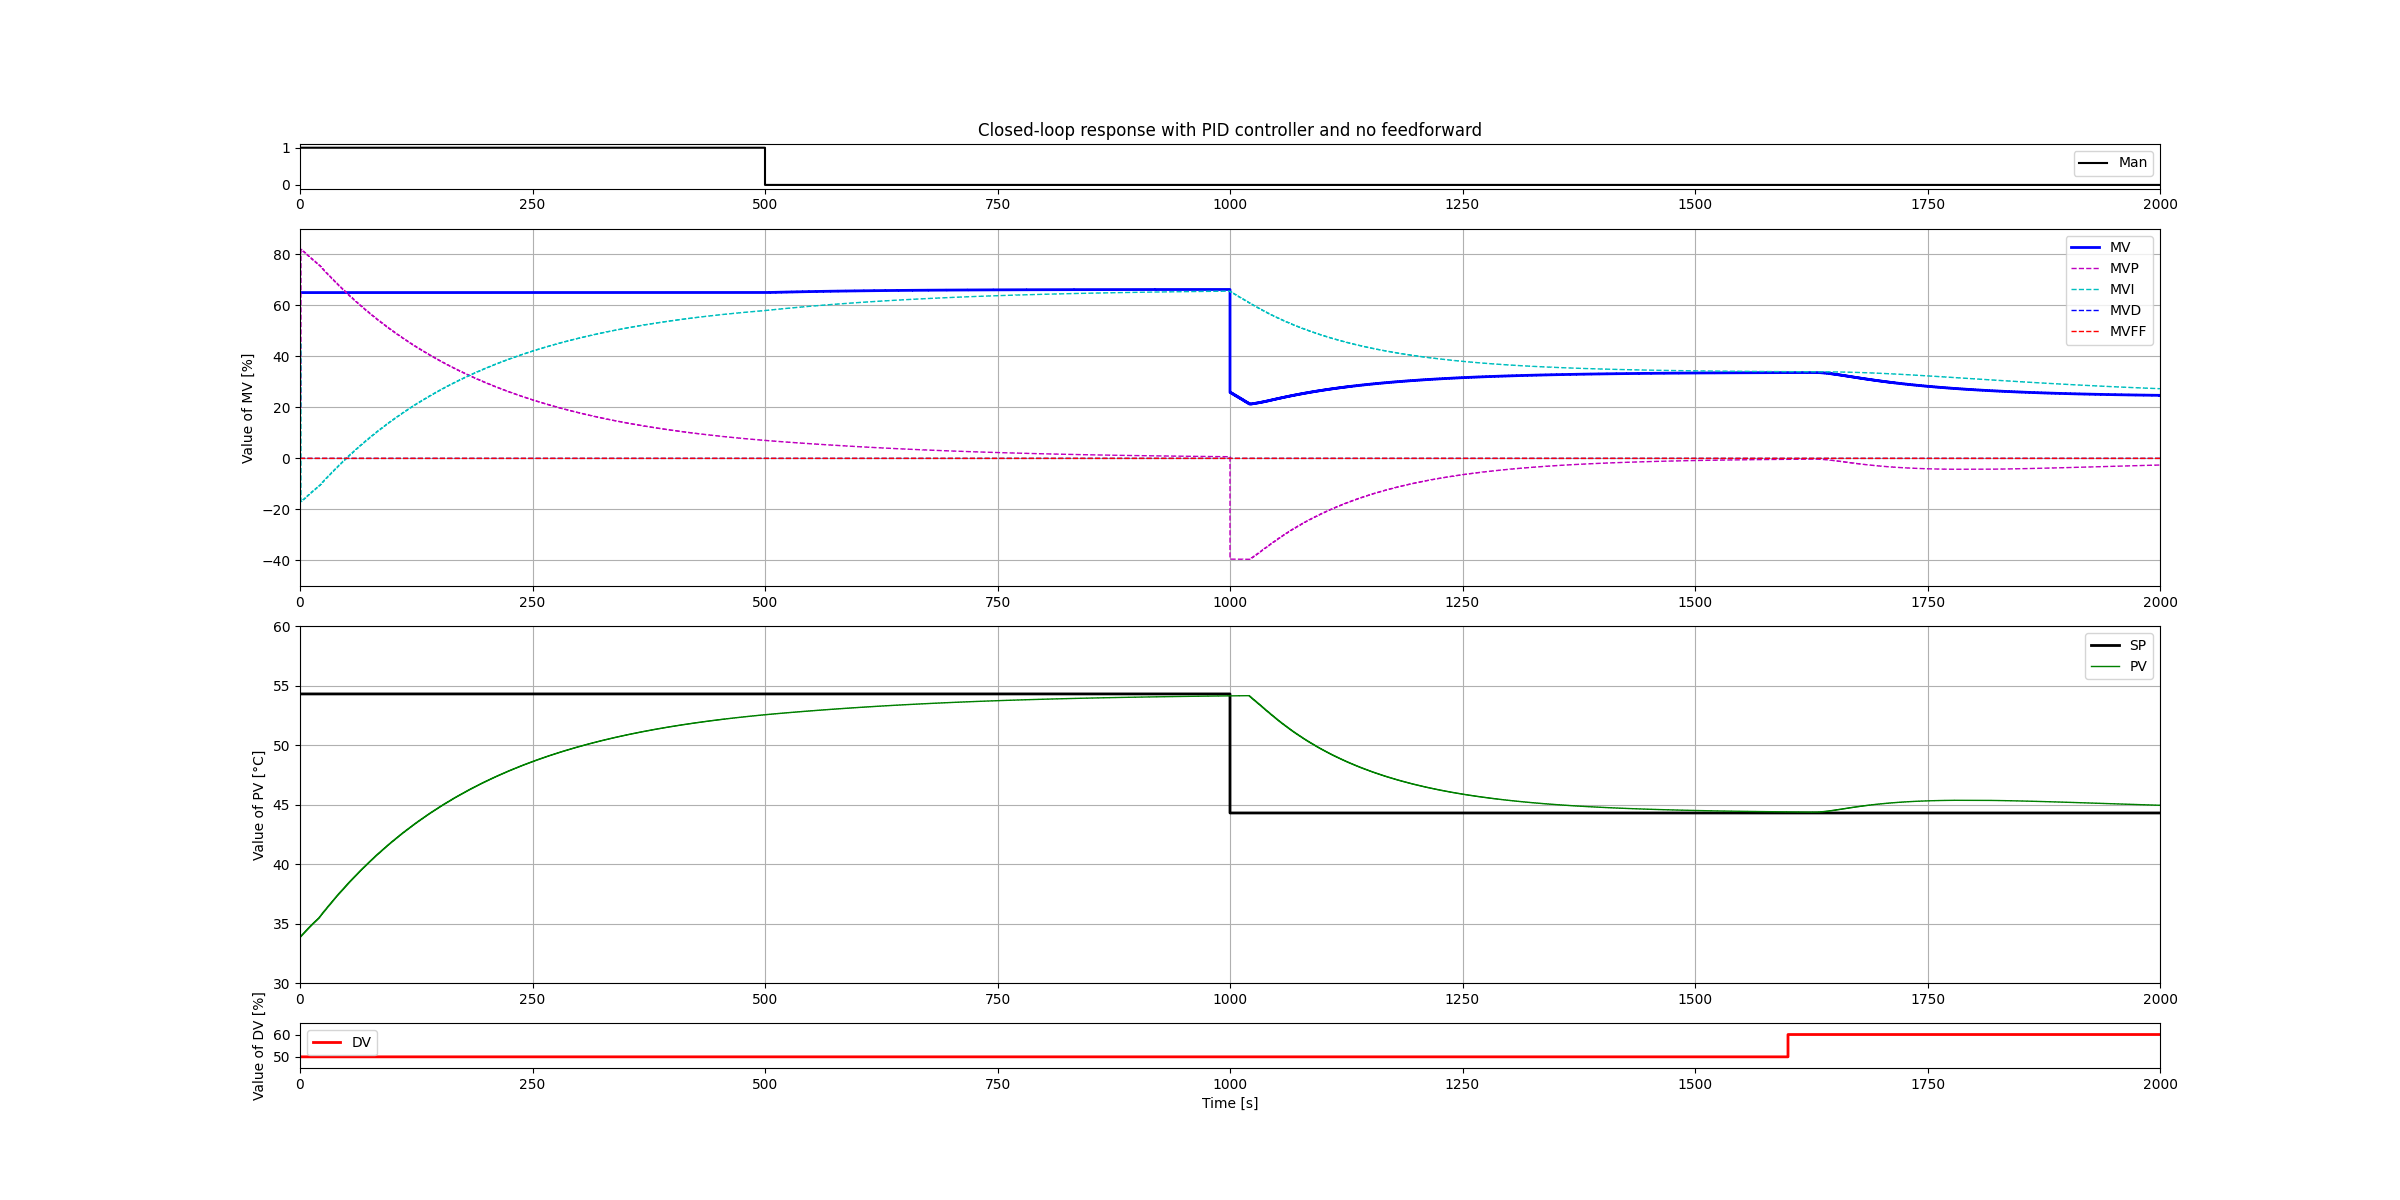
\includegraphics[width=0.9\textwidth]{../Plots/Simulation_scenario_5.png}
    \caption{Réponse à boucle fermée sans FeedForward}
    \label{fig:Simulation_CLP_no_FF}
\end{figure}
La Figure \ref{fig:Simulation_CLP_no_FF} utilise le mode manuel les quelques 500 premières secondes le temps d'amener $PV$ suffisement proche de $SP$, le mode automatique se charge de stabiliser $PV$.\\
On remarque tout de suite la réponse de $MV$ sur le step de $SP$, qui forme un pic avec un angle.
Nous pouvons enfait expliquer cela par la présence notable du délai $\theta_P = 20\,s$ entre $SP$ et $PV$.
En introduisant une erreur négative, l'action proportionnelle $MV_P = K_C \, E$ diminue mais l'erreur ne commencera à être compensée que après un délai $\theta_P$.
L'action intégrale $MV_I$, elle, diminue progressivement dès lors qu'elle accumule une erreur négative, faisant apparaître cette forme particulière sur $MV$.

Sans feedforward et comme mentionné précedement, une perturbation est bien relfetée sur $PV$.
$MV_P$ va suivre l'erreur introduite et automatiquement diminuer $MV$.
Encore une fois, l'action intégrale accumule cette erreur négative permettant à $MV$ de se stabiliser à une puissance de chauffe et ainsi faire retourner petit à petit $PV$ à la consigne $SP$.

\subsection{Réponse à une perturbation \texorpdfstring{$DV$}{DV} \& changement de consigne \texorpdfstring{$SP$}{SP} en mode automatique avec FF}
\begin{figure}[H]
    \centering
    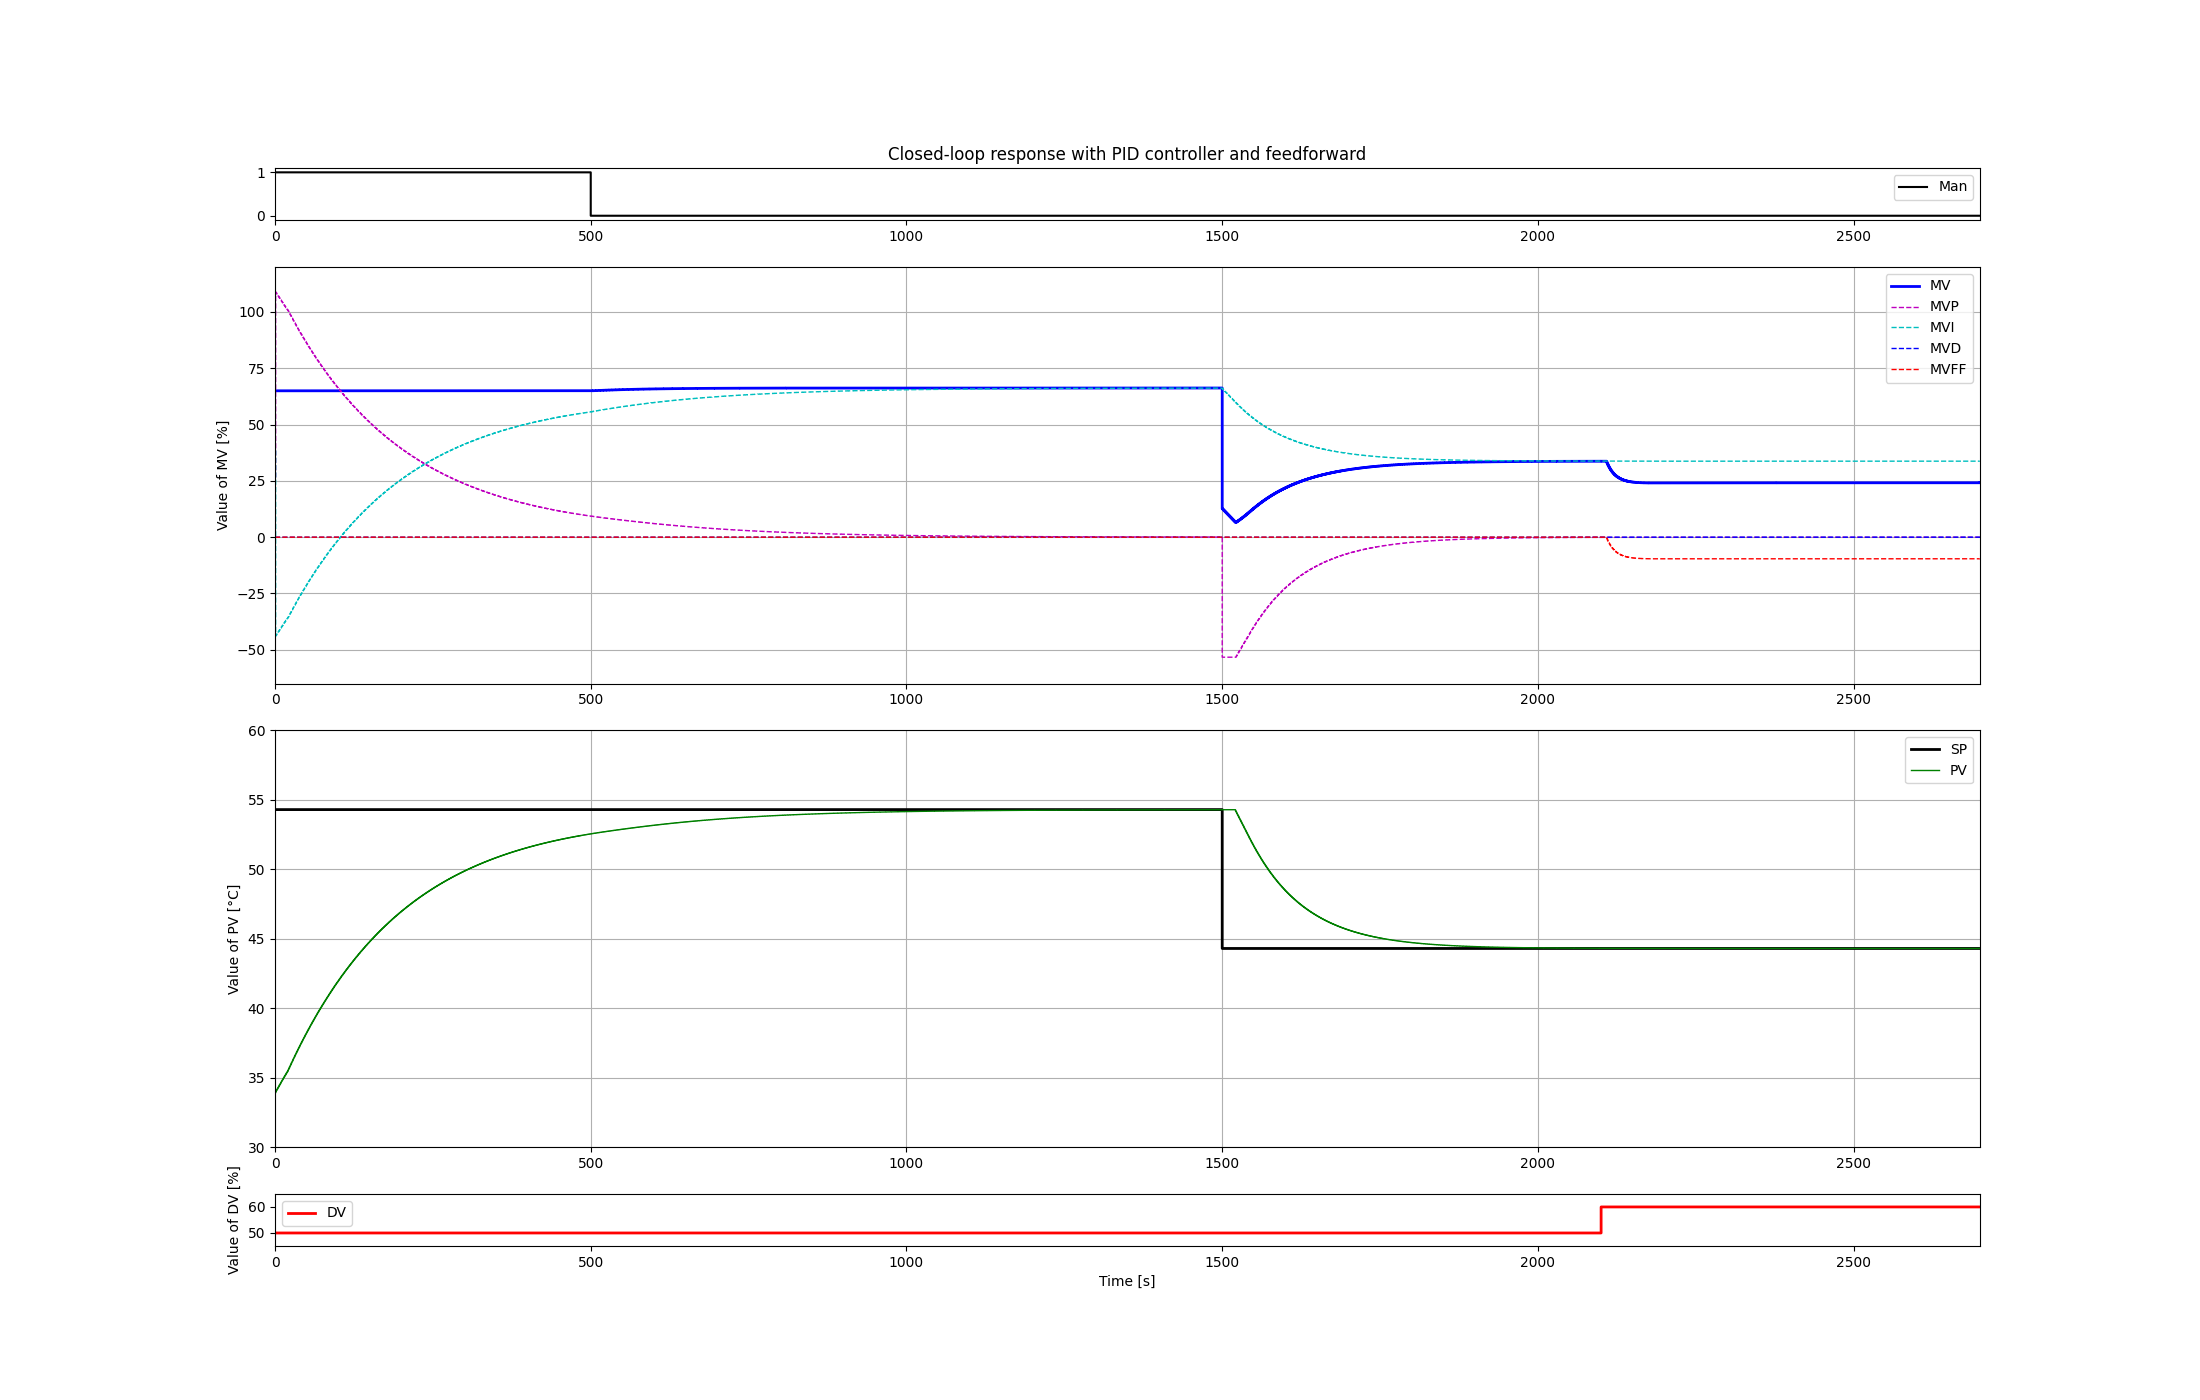
\includegraphics[width=0.9\textwidth]{../Plots/Simulation_scenario_7.png}
    \caption{Réponse à boucle fermée avec FeedForward}
    \label{fig:Simulation_CLP_FF}
\end{figure}
Sur la Figure \ref{fig:Simulation_CLP_FF} est représenté tout ce qui a été dit précedement notamment l'anticipation de la perturbation par le feedforward lorsque $MV_{FF}$ est diminué.
Encore une fois, le délai entre perturbation $DV$ et le feedforward $MV_{FF}$ est réduit à $\theta_{FF} = 9\,s$.

\subsection{Influence de \texorpdfstring{$\alpha$}{alpha} et \texorpdfstring{$\gamma$}{gamma}}
\begin{figure}[H]
    \centering
    \begin{subfigure}[b]{0.48\textwidth}
        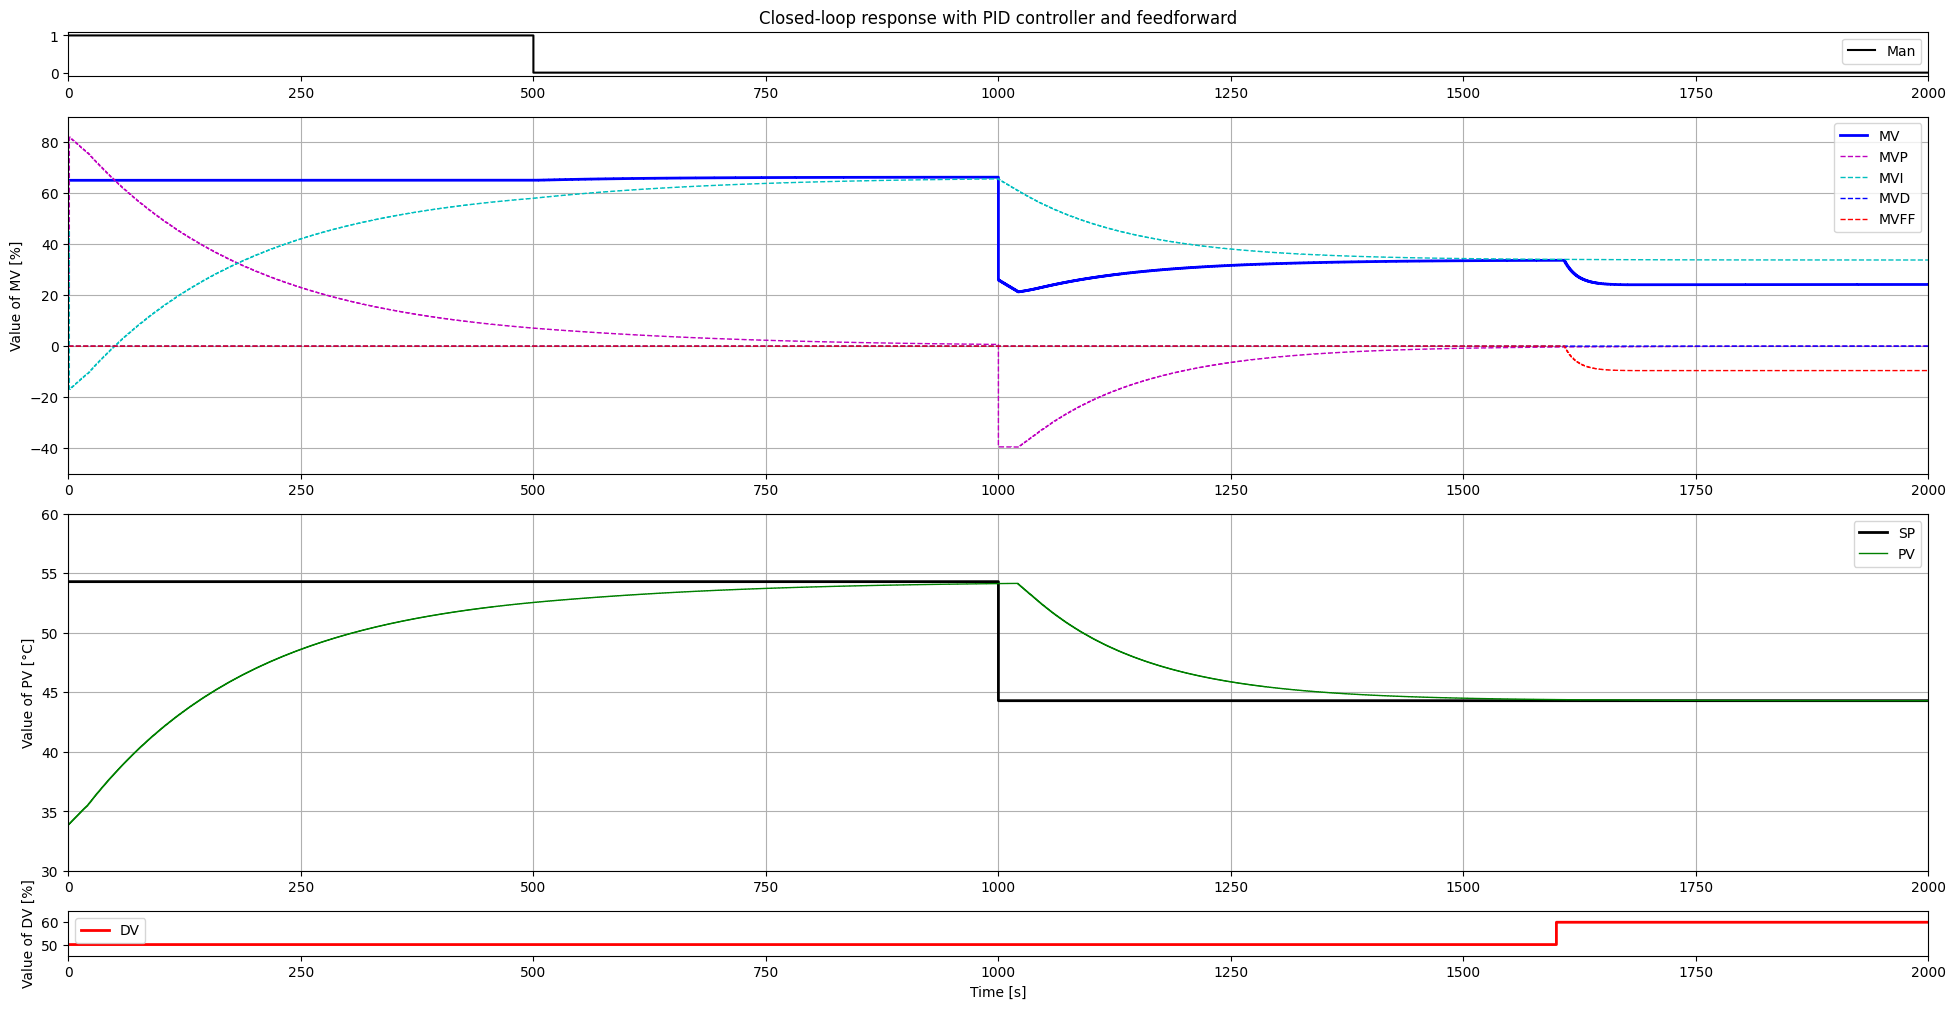
\includegraphics[width=\textwidth]{../Plots/Simulation_scenario_7_alpha=0.2.png}
        \caption{$\alpha = 0.2$}
    \end{subfigure}
    \begin{subfigure}[b]{0.48\textwidth}
        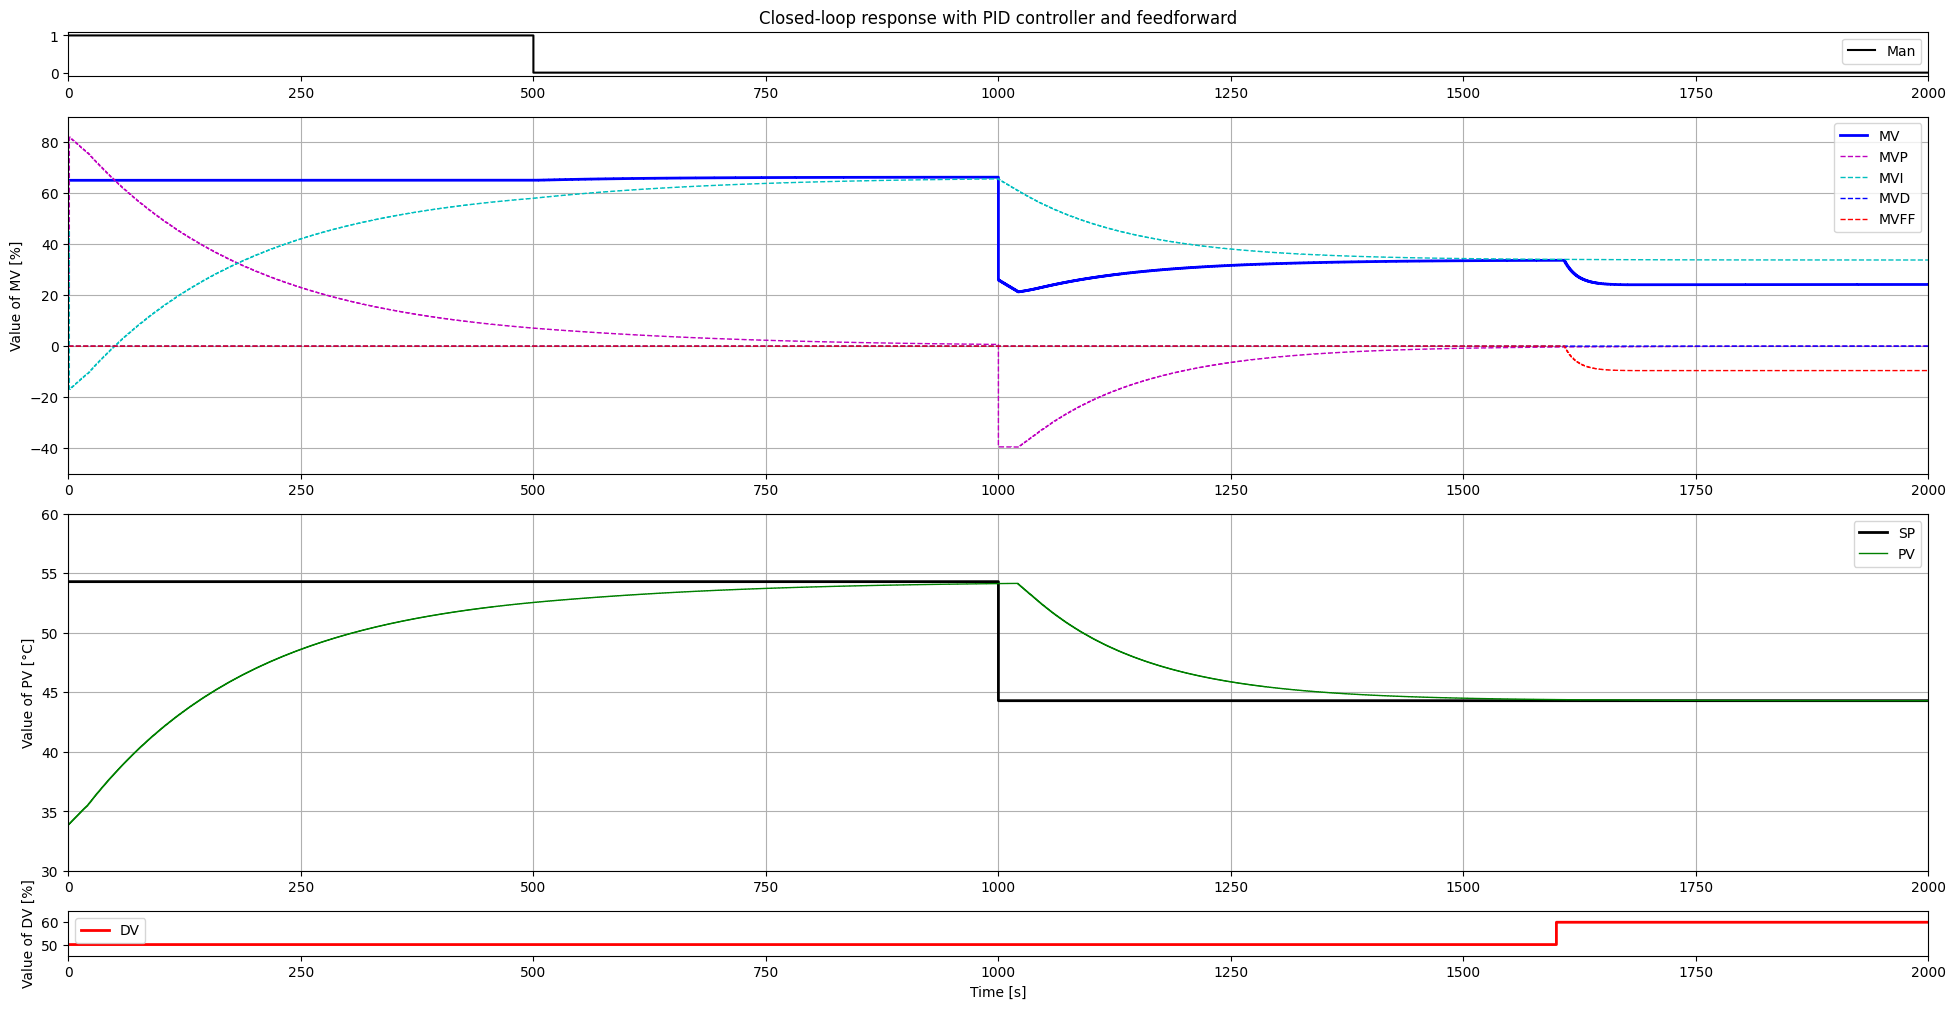
\includegraphics[width=\textwidth]{../Plots/Simulation_scenario_7_alpha=1.png}
        \caption{$\alpha = 1$}
    \end{subfigure}
    \caption{Influence de $\alpha$ sur la boucle fermée}
    \label{fig:Simulation_alpha_influence}
\end{figure}
La Figure \ref{fig:Simulation_alpha_influence} permet de montrer que, \underline{pour notre système}, $\alpha$ n'a aucune influence.
Il n'intervient que dans la limitation du gain haute fréquence de l'action dérivée. Or notre régulateur agit comme un régulateur PI, donc l'action dérivée reste nulle tout le long de la simulation.

\begin{figure}[H]
    \centering
    \begin{subfigure}[b]{0.48\textwidth}
        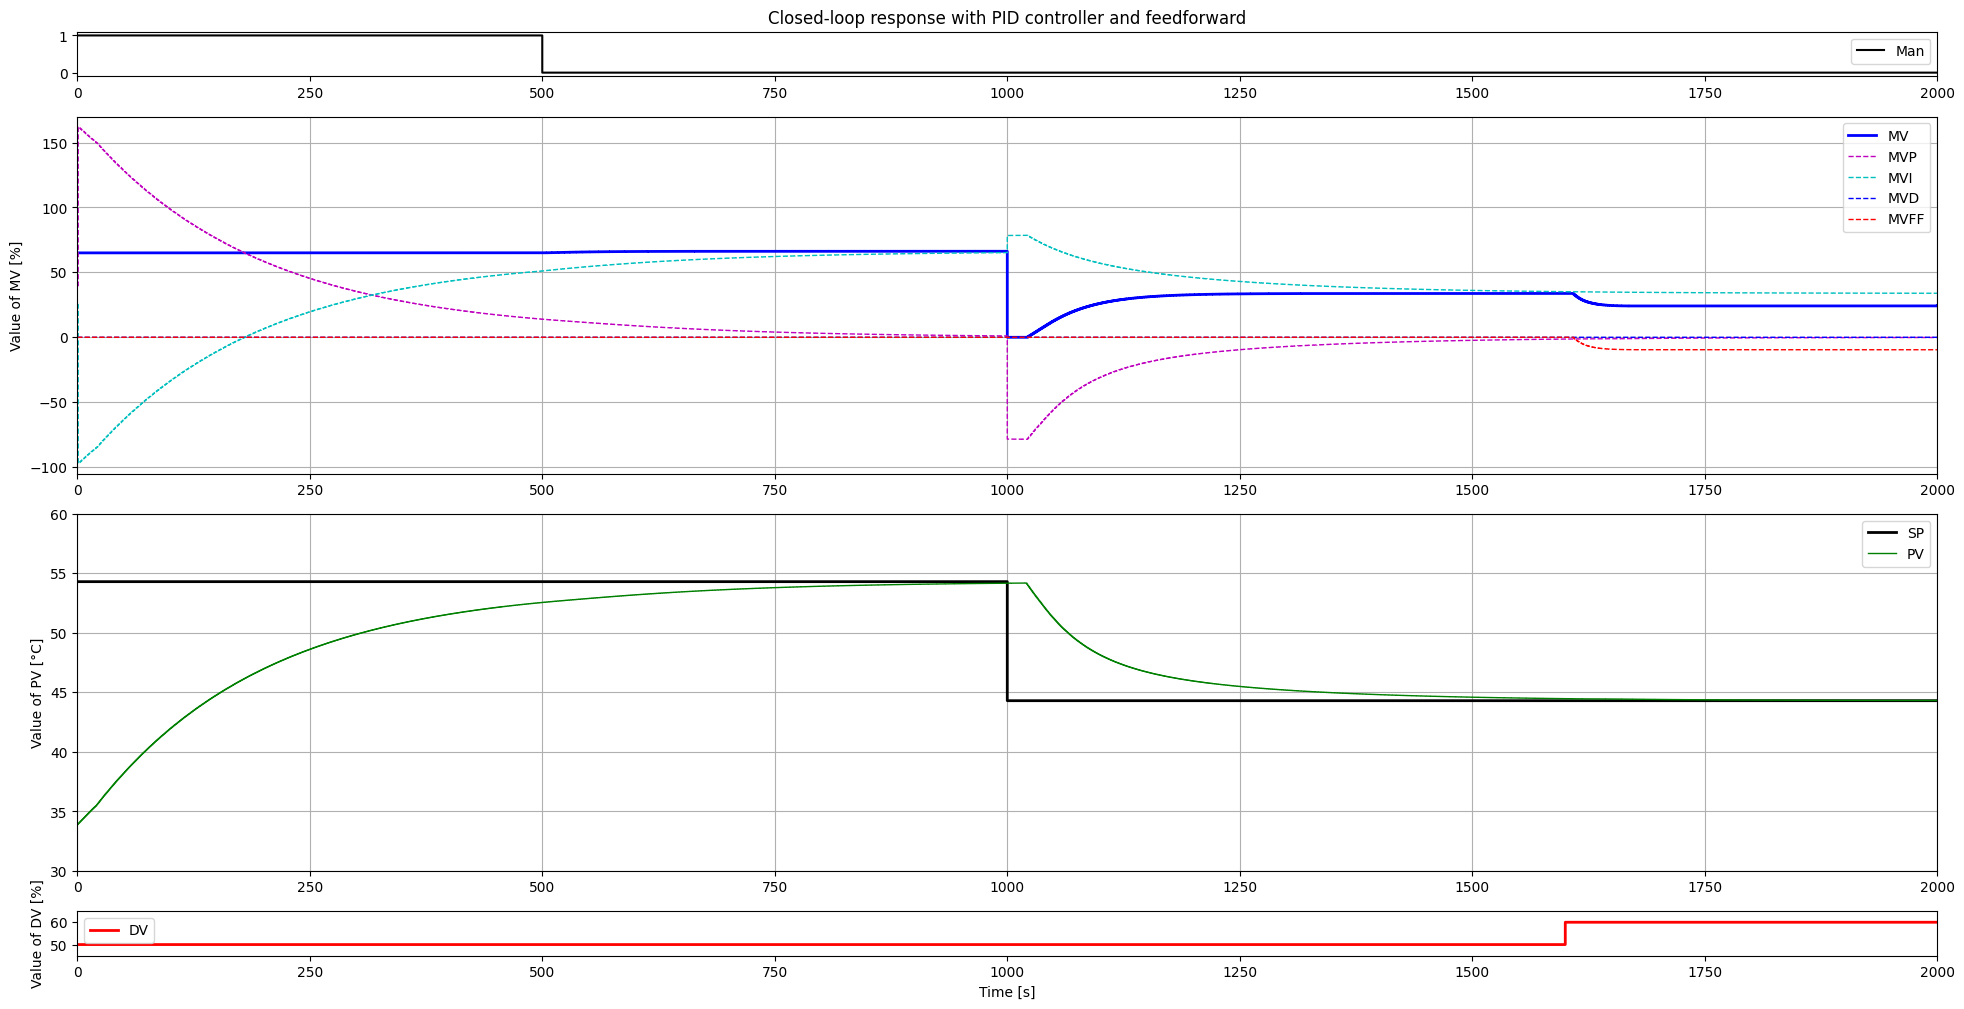
\includegraphics[width=\textwidth]{../Plots/Simulation_scenario_7_gamma=0.3.png}
        \caption{$\gamma = 0.3$}
    \end{subfigure}
    \begin{subfigure}[b]{0.48\textwidth}
        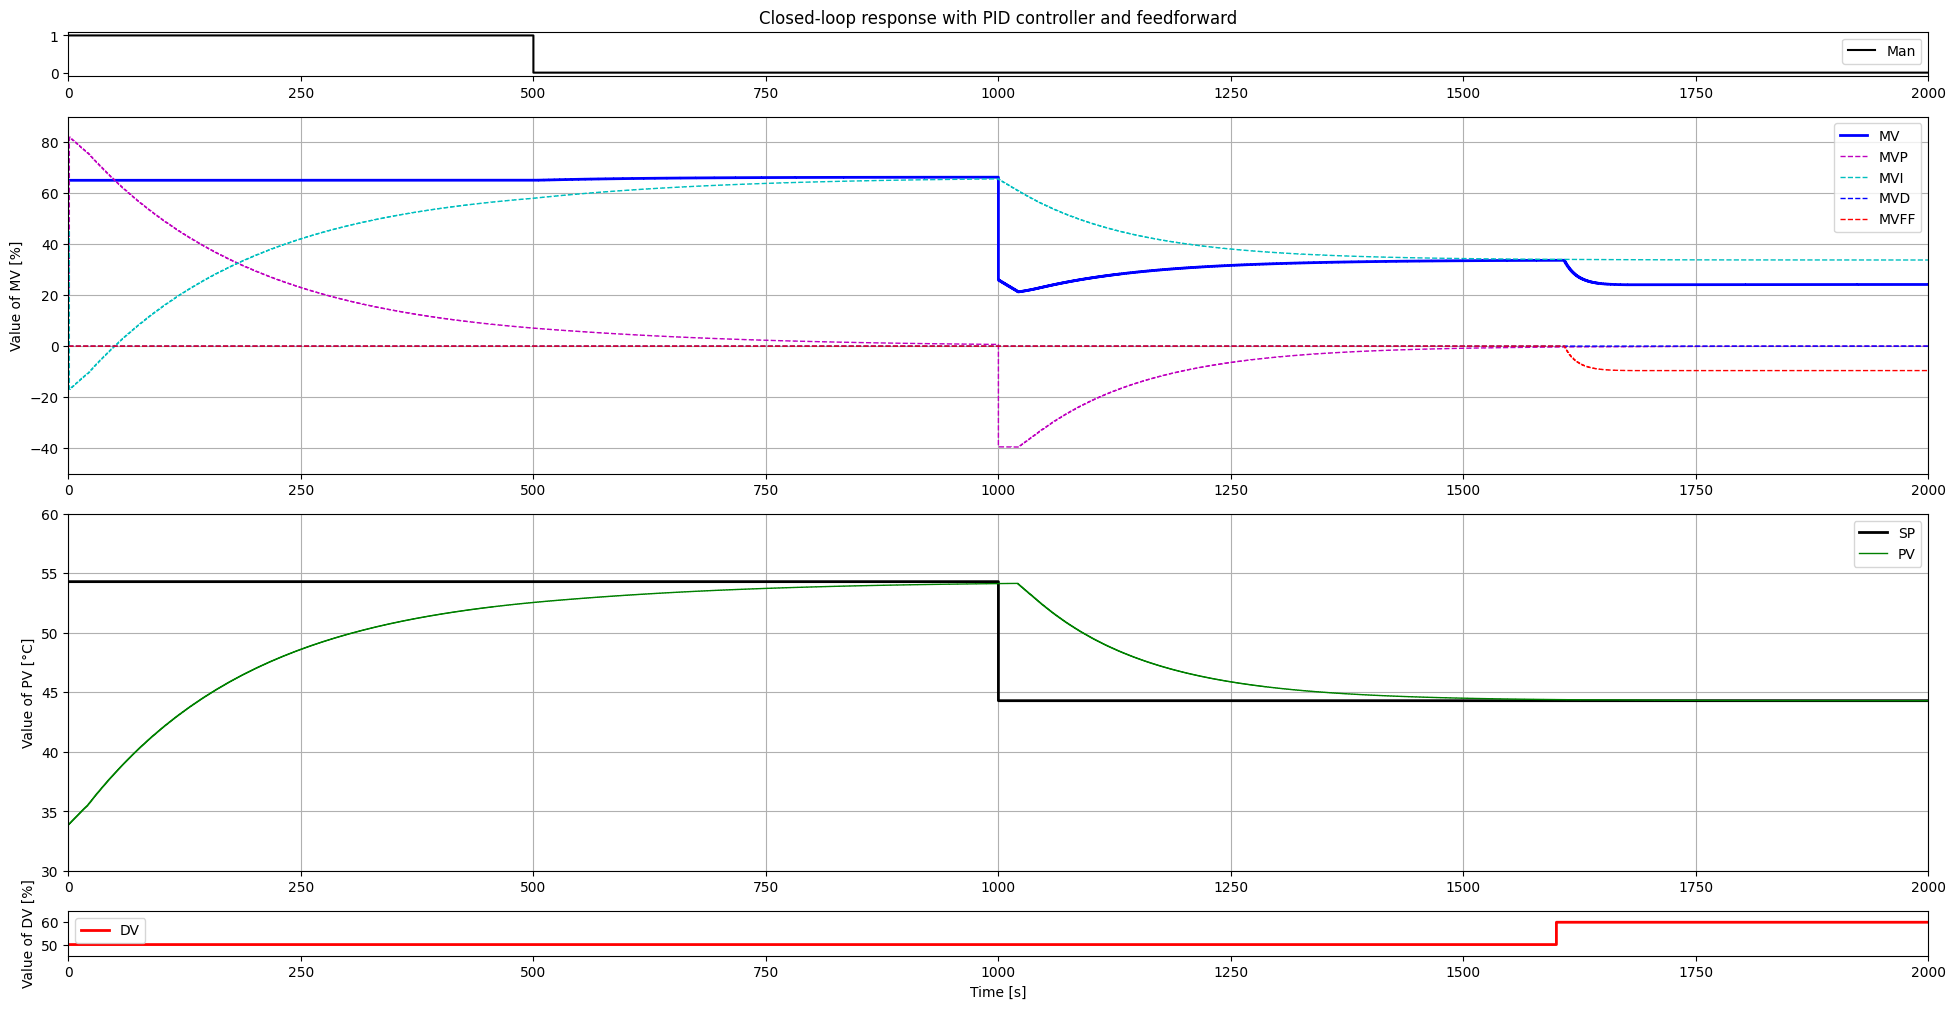
\includegraphics[width=\textwidth]{../Plots/Simulation_scenario_7_gamma=0.7.png}
        \caption{$\gamma = 0.7$}
    \end{subfigure}
    \caption{Influence de $\gamma$ sur la boucle fermée}
    \label{fig:Simulation_gamma_influence}
\end{figure}
Le paramètre $\gamma$ est utilisé dans l'optimisation IMC et fait par ce biais varier le gain du régulateur $K_C$.
\begin{equation*}
    K_C = \frac{1}{K_P} \, \frac{T_{1p} + T_{2p}}{\gamma \, T_{1p} + \theta}
\end{equation*}
Nous voyons effectivement sur la Figure \ref{fig:Simulation_gamma_influence} (a), qu'un $\gamma$ plus petit vient amplifier toutes les composantes de $MV$.
Il est alors également intéressant d'observer que l'action proportionnelle est plus grande et donc vient amener $MV$ à saturer lors du step sur la consigne.
L'action intégrale doit s'ajuster en augmentant sa valeur.\\
En se focalisant sur la phase transitoire de $PV$ lorsque le step est appliqué sur $SP$, nous pouvons noter une différence de temps de montée entre les deux simulations.
Le $\gamma$ plus petit arrive plus rapidement à 90\% de la valeur en régime établi.
Cela permet de confirmer le caractère plus aggressif du régulateur lorsque $\gamma$ est plus petit.

%---------- Données Expérimentales ----------%
\newpage
\section{Données Expérimentales}

Nous allons maintenant tester notre régulateur PID sur la plateforme afin de comparer son comportement en 
simulation à son comportement réel. Nous avons donc mis en place 4 scénarios qui permettront de comparer 
tous les cas de figure : 
\begin{enumerate}
	\item Le $1^{er}$ scénario permet de tester le fonctionnement du régulateur en boucle ouverte (mode manuel) sans FeedForward en observant sa réponse à un step de $10\%$ sur $DV$.
	\begin{python*}
		SPPath = {0: PV0} 
		ManPath = {0: True, TSim: True} # Mode manuel actif toute la simulation
		MVManPath = {0: MV0, TSim: MV0} # MV manuel reste constant
		DVPath = {0: DV0, 1300: DV0 + 10} # Step de 10% après 1300 secondes
		FF = False # Pas de FeedForward
		ManFF = False # Pas de prise en compte du FeedForward 
	\end{python*}
	\item Le $2^{ème}$ scénario permet de de tester le fonctionnement du régulateur en boucle ouverte et avec FeedForward en observant 
	sa réponse à un step de $10\%$ sur $DV$.
	\begin{python*}
		SPPath = {0: PV0}
		ManPath = {0: True, TSim: True} #Mode manuel actif toute la simulation
		MVManPath = {0: MV0, TSim: MV0} # MV manuel reste constant
		DVPath = {0: DV0, 1300: DV0 + 10} # Step de 10% après 1300 secondes
		FF = True # FeedForward activé
		ManFF = True # Prise en compte du FeedForward
	\end{python*}
	\item Le $3^{ème}$ scénario permet de tester le fonctionnement du régulateur en boucle fermée (mode automatique) sans FeedForward en observant sa réponse
	à un step de $-10\%$ sur $SP$ puis un step de $10\%$ sur $DV$.
	\begin{python*}
		SPPath = {0: PV0 + 5, 1000: PV0 - 5} # Step de -10% après 1000 secondes
		ManPath = {0: True, 500: False, TSim: False} 
		MVManPath = {0: MV0+15, TSim: MV0+15}
		DVPath = {0: DV0, 1600: DV0 + 10} # Step de 10% après 1600 secondes
		FF = False # Pas de FeedForward
		ManFF = False 
	\end{python*}
	\item Le $4^{ème}$ scénario permet de compléter le scnéario précédant en testant le fonctionnement du régulateur en boucle fermée FeedForward en observant sa réponse à un step
	de $-10\%$ sur $SP$ puis à un step de $10\%$ sur $DV$.
	\begin{python*}
		SPPath = {0: PV0 + 5, 1000: PV0 - 5} #Step de -10% après 1000 secondes
		ManPath = {0: True, 500: False, TSim: False} # Mode automatique après 500 secondes
		MVManPath = {0: MV0+15, TSim: MV0+15} 
		DVPath = {0: DV0, 1600: DV0 + 10} # Step de 10% après 1600 secondes
		FF = True # FeedForward activé
		ManFF = False 
	\end{python*}
\end{enumerate}

\subsection{Scénario 1}
\begin{figure}[H]
	\centering
	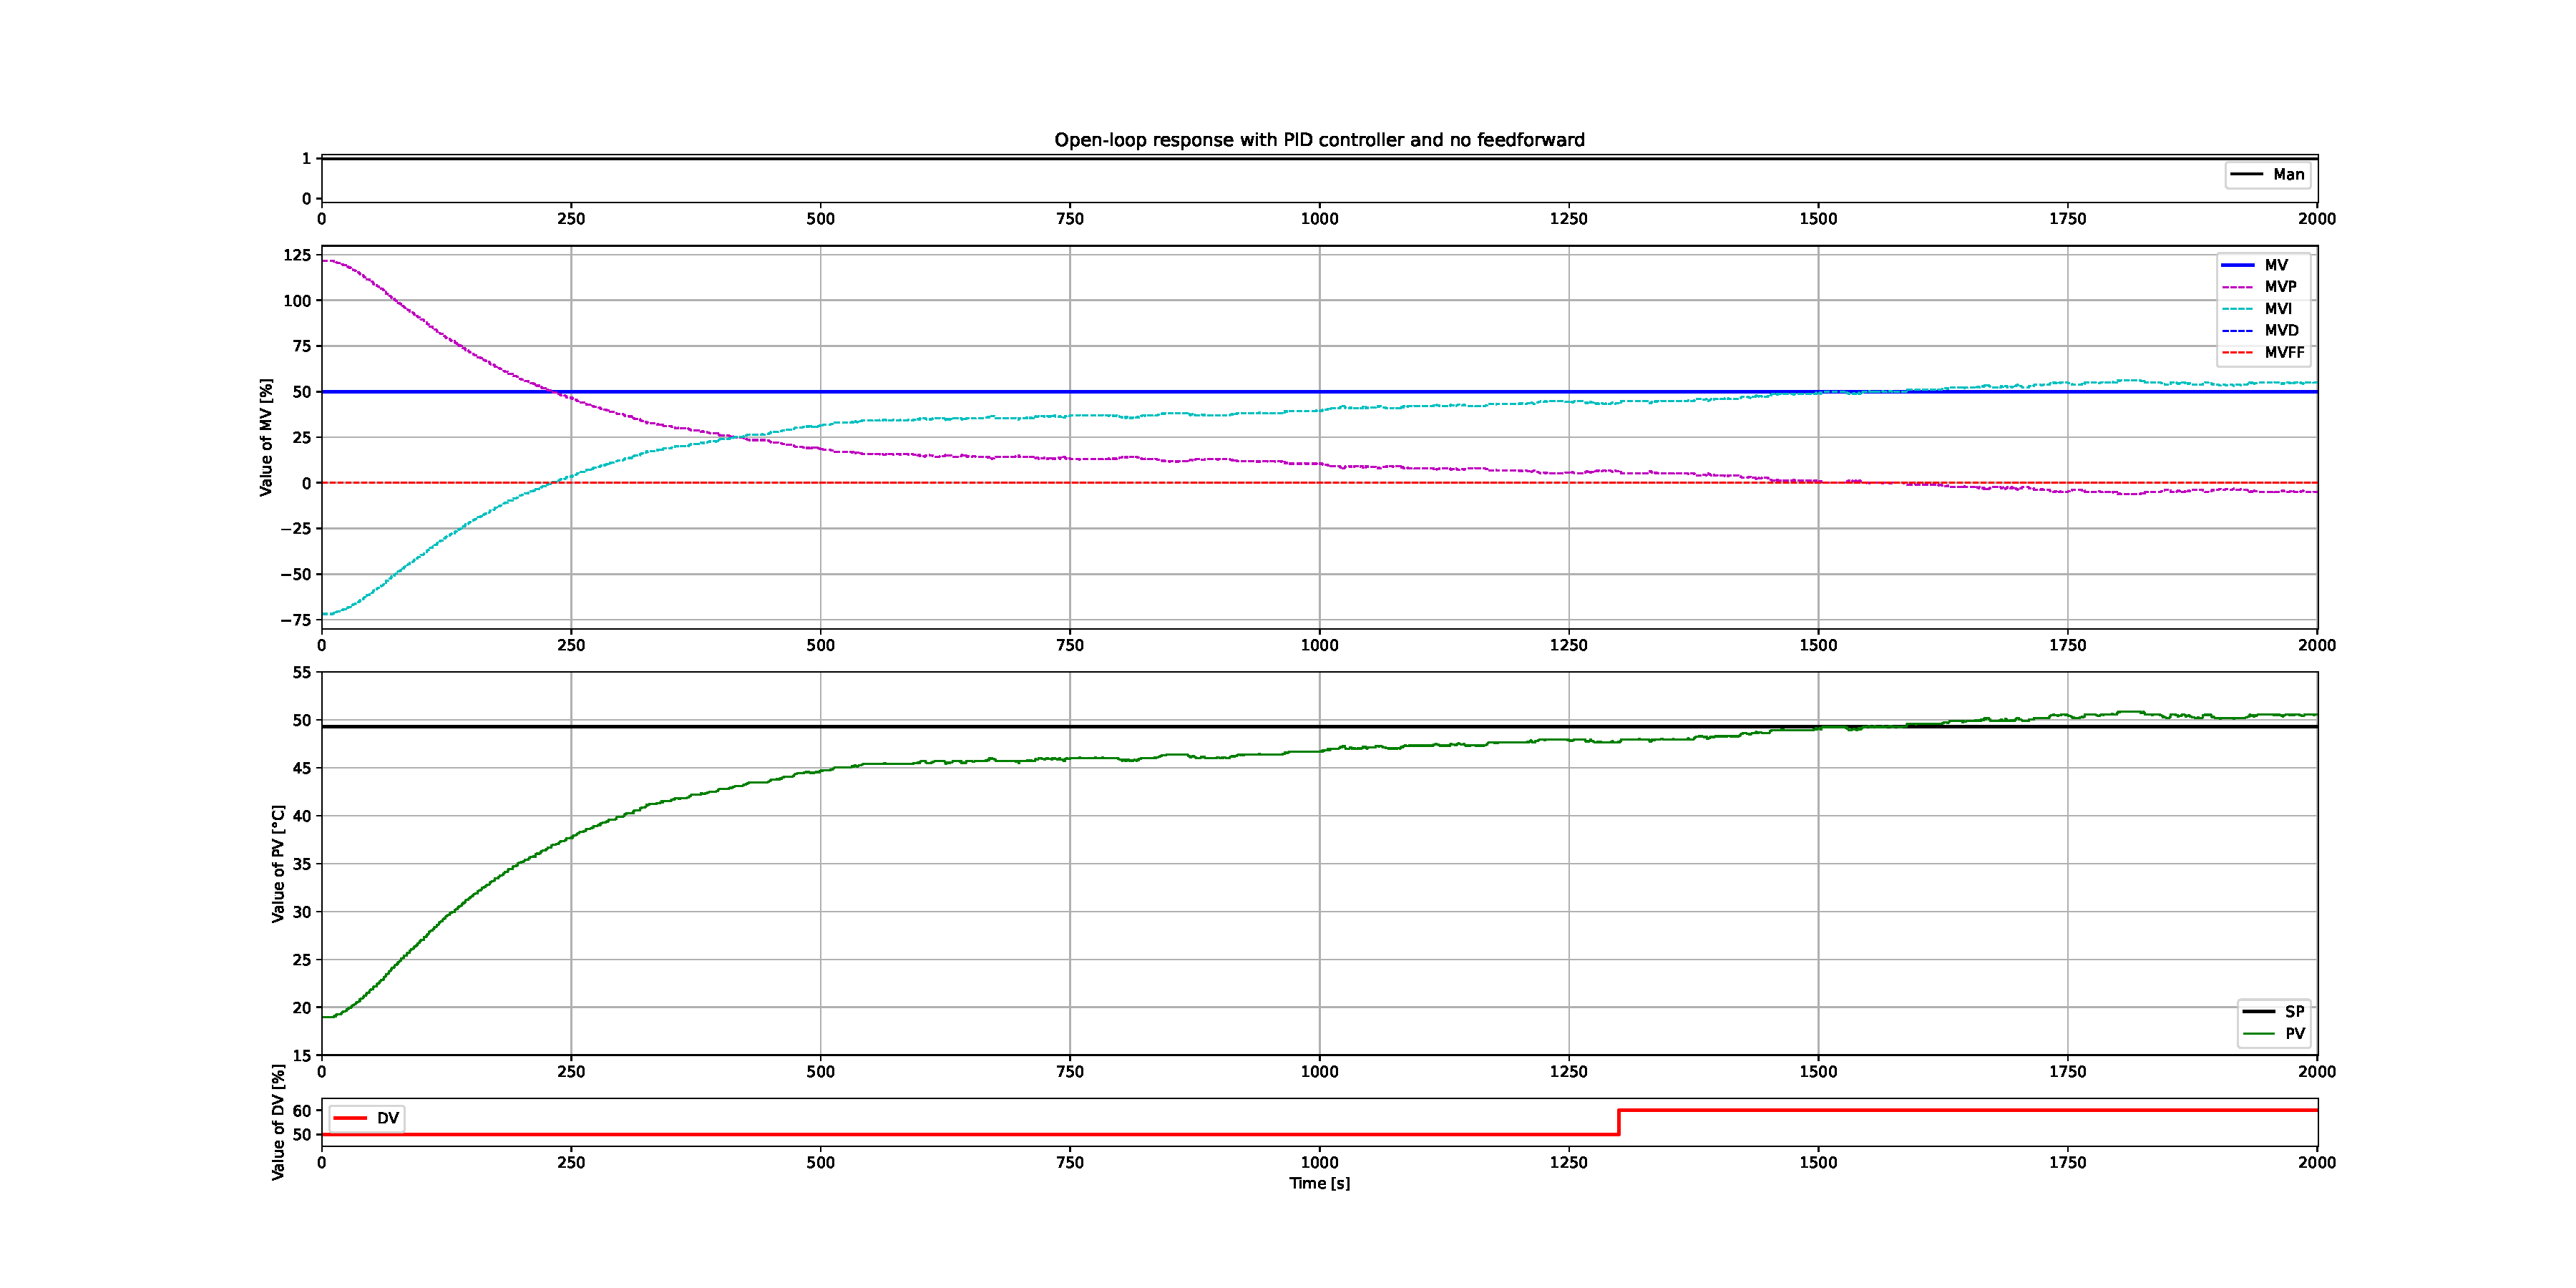
\includegraphics[width=1\textwidth]{../Plots/Experiment_scenario_2_2024-03-30-20h20.pdf}
	\caption{Données expérimentales du $1^{er}$ scénario}
	\label{fig:exp_scenario1}
\end{figure}
\begin{figure}[H]
	\centering
	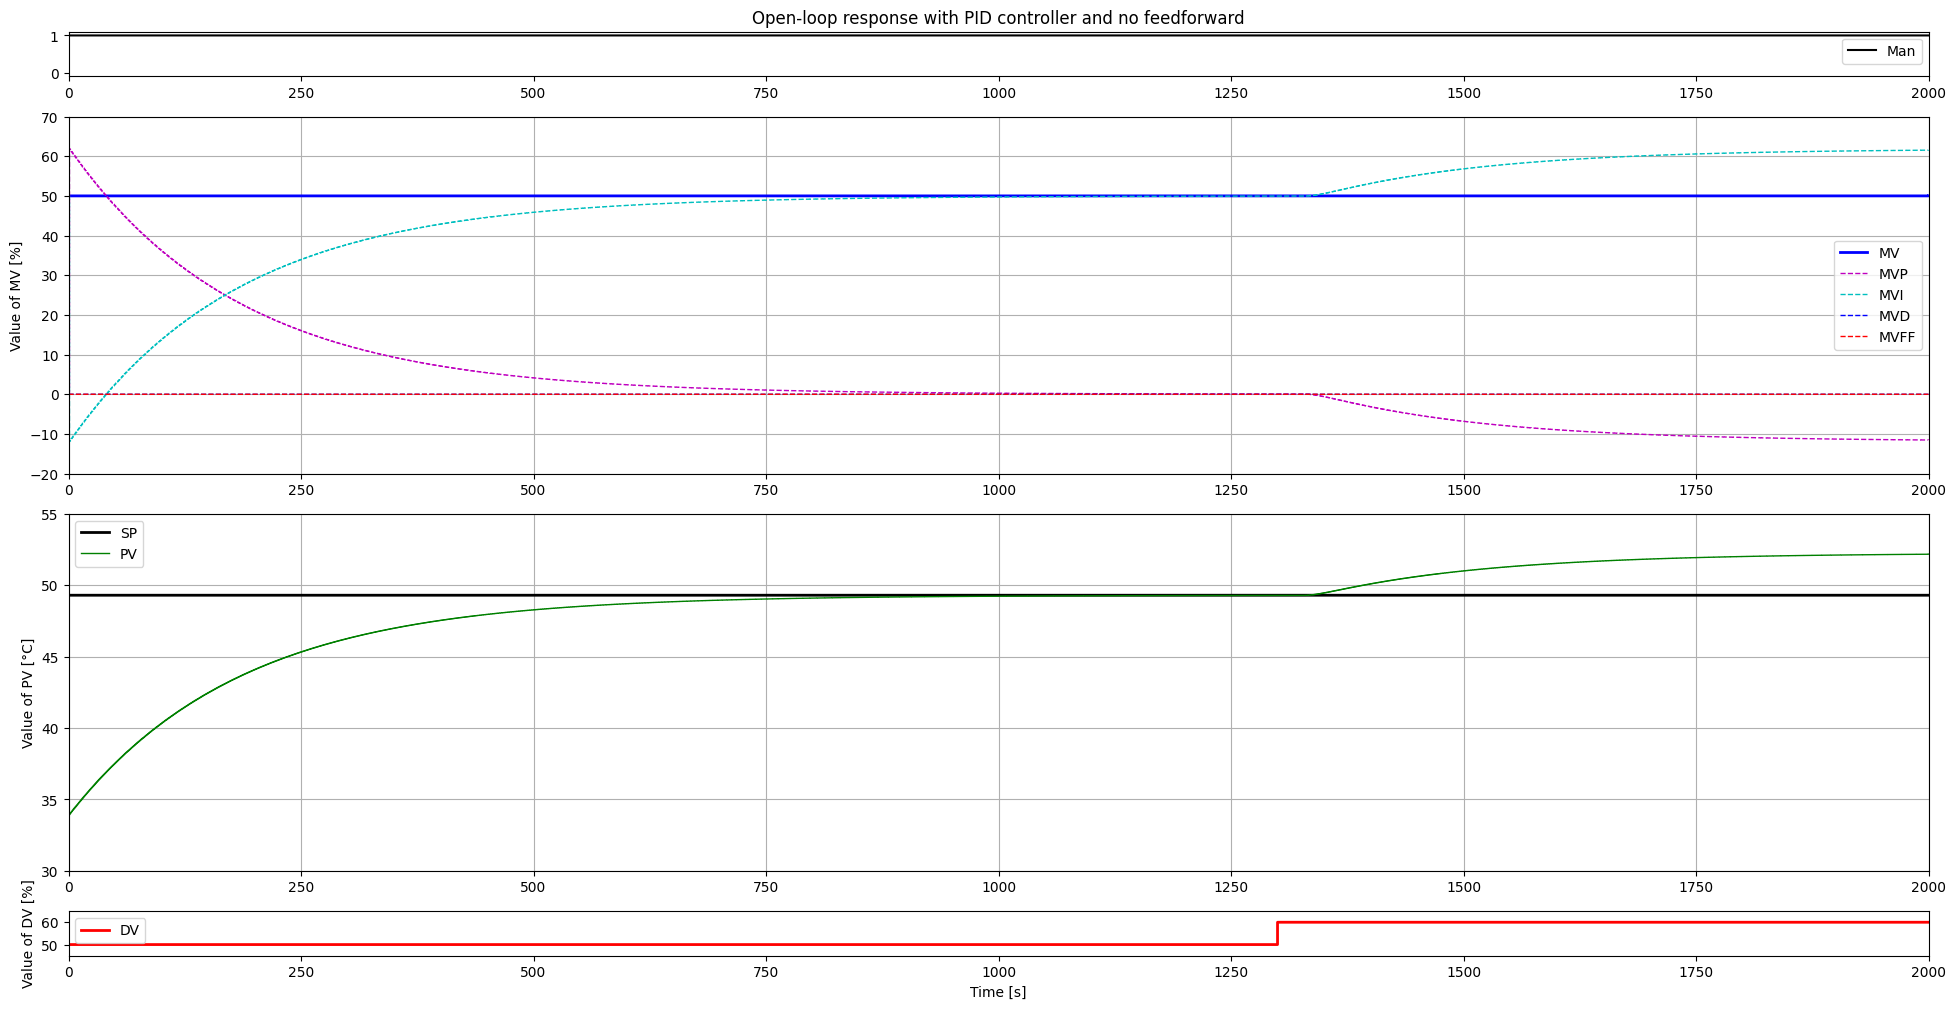
\includegraphics[width=0.8\textwidth]{figures/scenario2.png}
	\caption{Données de la simulation du $1^{er}$ scénario}
	\label{fig:sim_scenario1}
\end{figure}

On peut observer que le $PV$ n'a pas atteint la valeur de consigne ($SP$) avant le step de $10\%$ sur $DV$. Cela est dû au fait que, pour l'expérience,
la valeur du $PV$ à $t = 0s$ est de $\sim 18\degree C$ tandis que pour la simulation, il est de $\sim 34\degree C$. Néanmoins, une fois le step de $10\%$ sur $DV$ effectué,
la valeur du $PV$ converge jusqu'à la valeur de consigne et la dépasse à $t = 1500s$ ce qui correspond à un retard par rapport à la simulation $\sim \Delta t = 75s$. 
\\Une autre observation importante concerne la forme de la courbe $PV$ qui suggère un comportement typique d'un système du second ordre. Cependant, l'analyse des dynamiques du système 
lors du $1^{er}$ laboratoire avait révélé une seconde constante de temps très faible, $T_2P \sim 10^{-12}$. $T_{2P}$ étant négligeable, nous avions conclu que notre système se comportait
plutôt comme un système du premiere ordre en réponse à un changement sur $MV$. Selon nous, une des causes de ce changement de forme de courbe serait la température plus basse de la pièce qui affecterait 
l'inertie thermique du capteur de température. L'humidité de la pièce pourrait aussi être facteur puisque celle-ci affecte la conductivité thermique de l'air 
ambiant et donc pourrait aussi impacter l'inertie thermique du capteur.

\subsection{Scénario 2}

\begin{figure}[H]
	\centering
	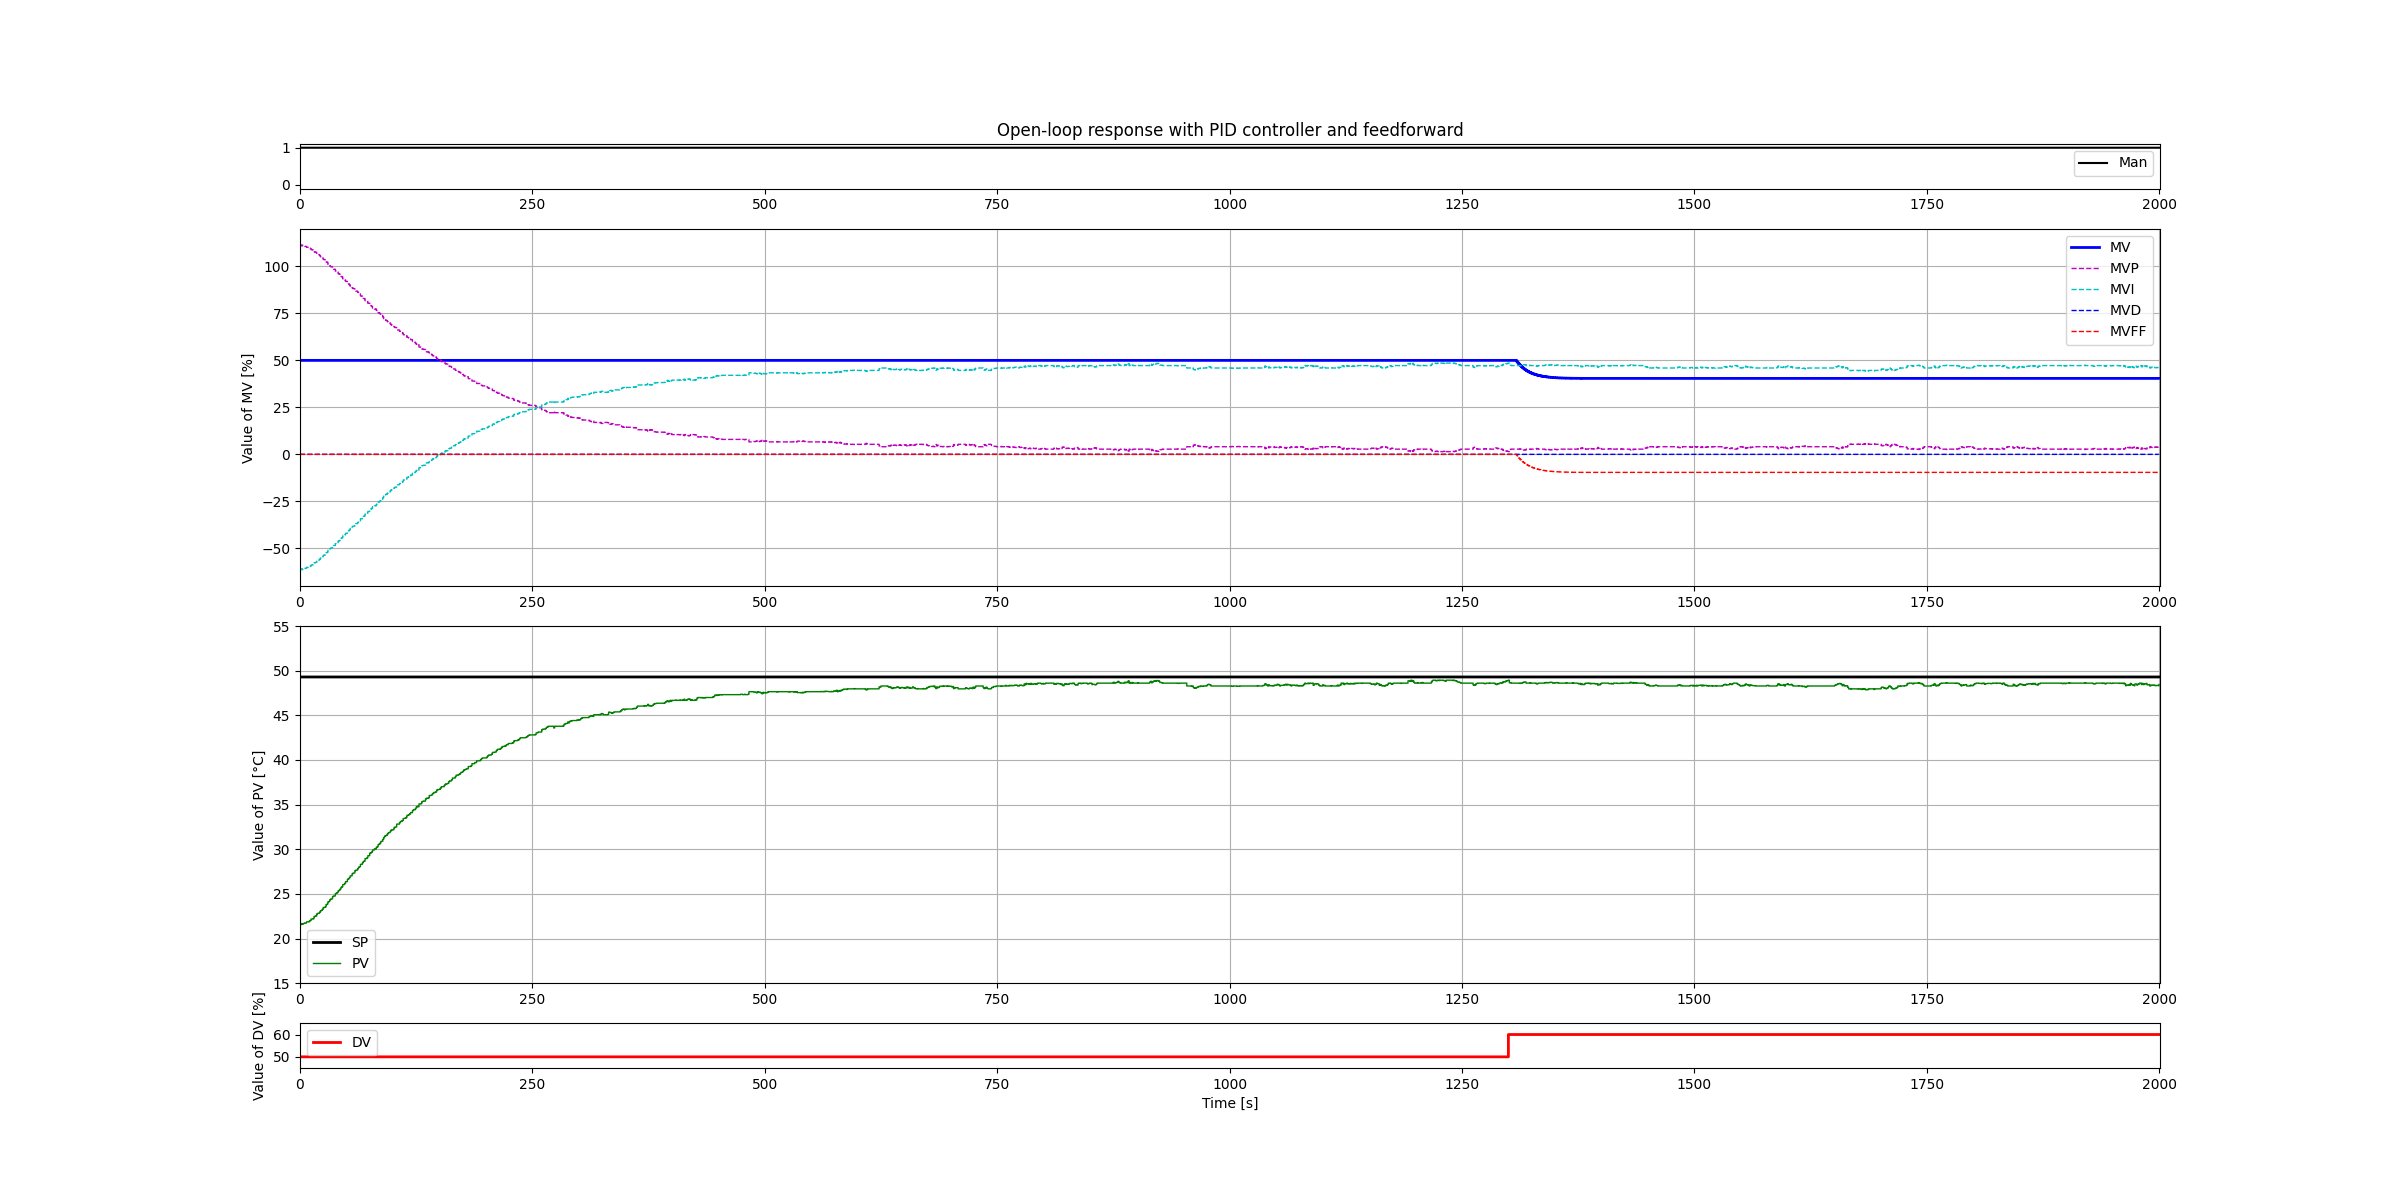
\includegraphics[width=1\textwidth]{../Plots/Experiment_scenario_3_2024-03-30-19h18.png}
	\caption{Données expérimentales du $2^{ème}$ scénario}
	\label{fig:exp_scenario2}
\end{figure}
\begin{figure}[H]
	\centering
	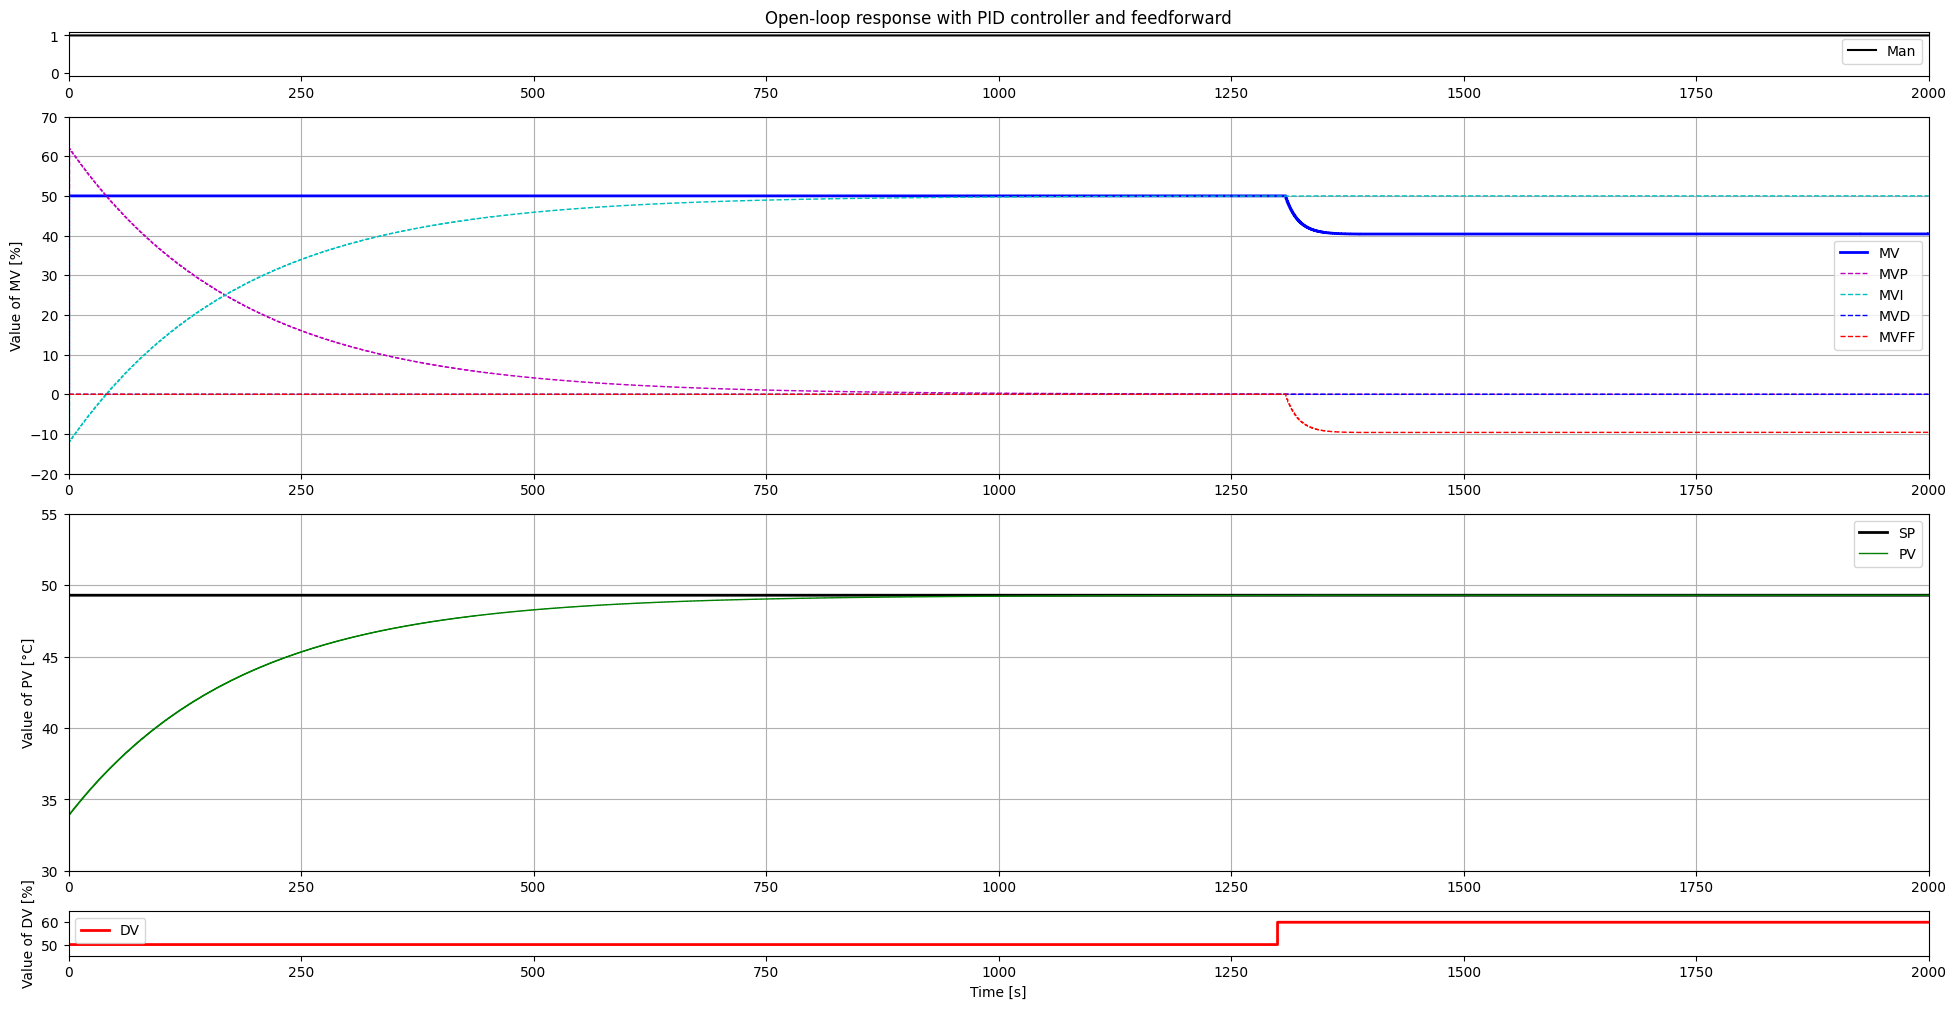
\includegraphics[width=0.8\textwidth]{figures/scenario3.png}
	\caption{Données de la simulation du $2^{ème}$ scénario}
	\label{fig:sim_scenario2}
\end{figure}

Dans ce scénario, tout comme dans le précédent(\ref{fig:exp_scenario1}), le système réagit plutôt comme un système du second ordre.
\\Toutefois, à la différence du scénario précédent, la valeur du $PV$ atteint à peu près au même moment la valeur de consigne ($SP$) que pour la simulation. Ceci est dû au fait
que la température du capteur n'a pas suffisamment pu redescendre entre les deux scénarios. En effet, la valeur de $PV$ à $t = 0s$ est de $\sim 22\degree C$ ce qui correspond 
à $4\degree C$ de plus que pour le scénario précédent. 
\\Mis à part ce détail, le système a bien répondu à la perturbation. L'utilisation du FeedForward a permis de neutraliser complètement l'effet du step de $10\%$ sur $DV$.

\subsection{Scénario 3}

\begin{figure}[H]
	\centering
	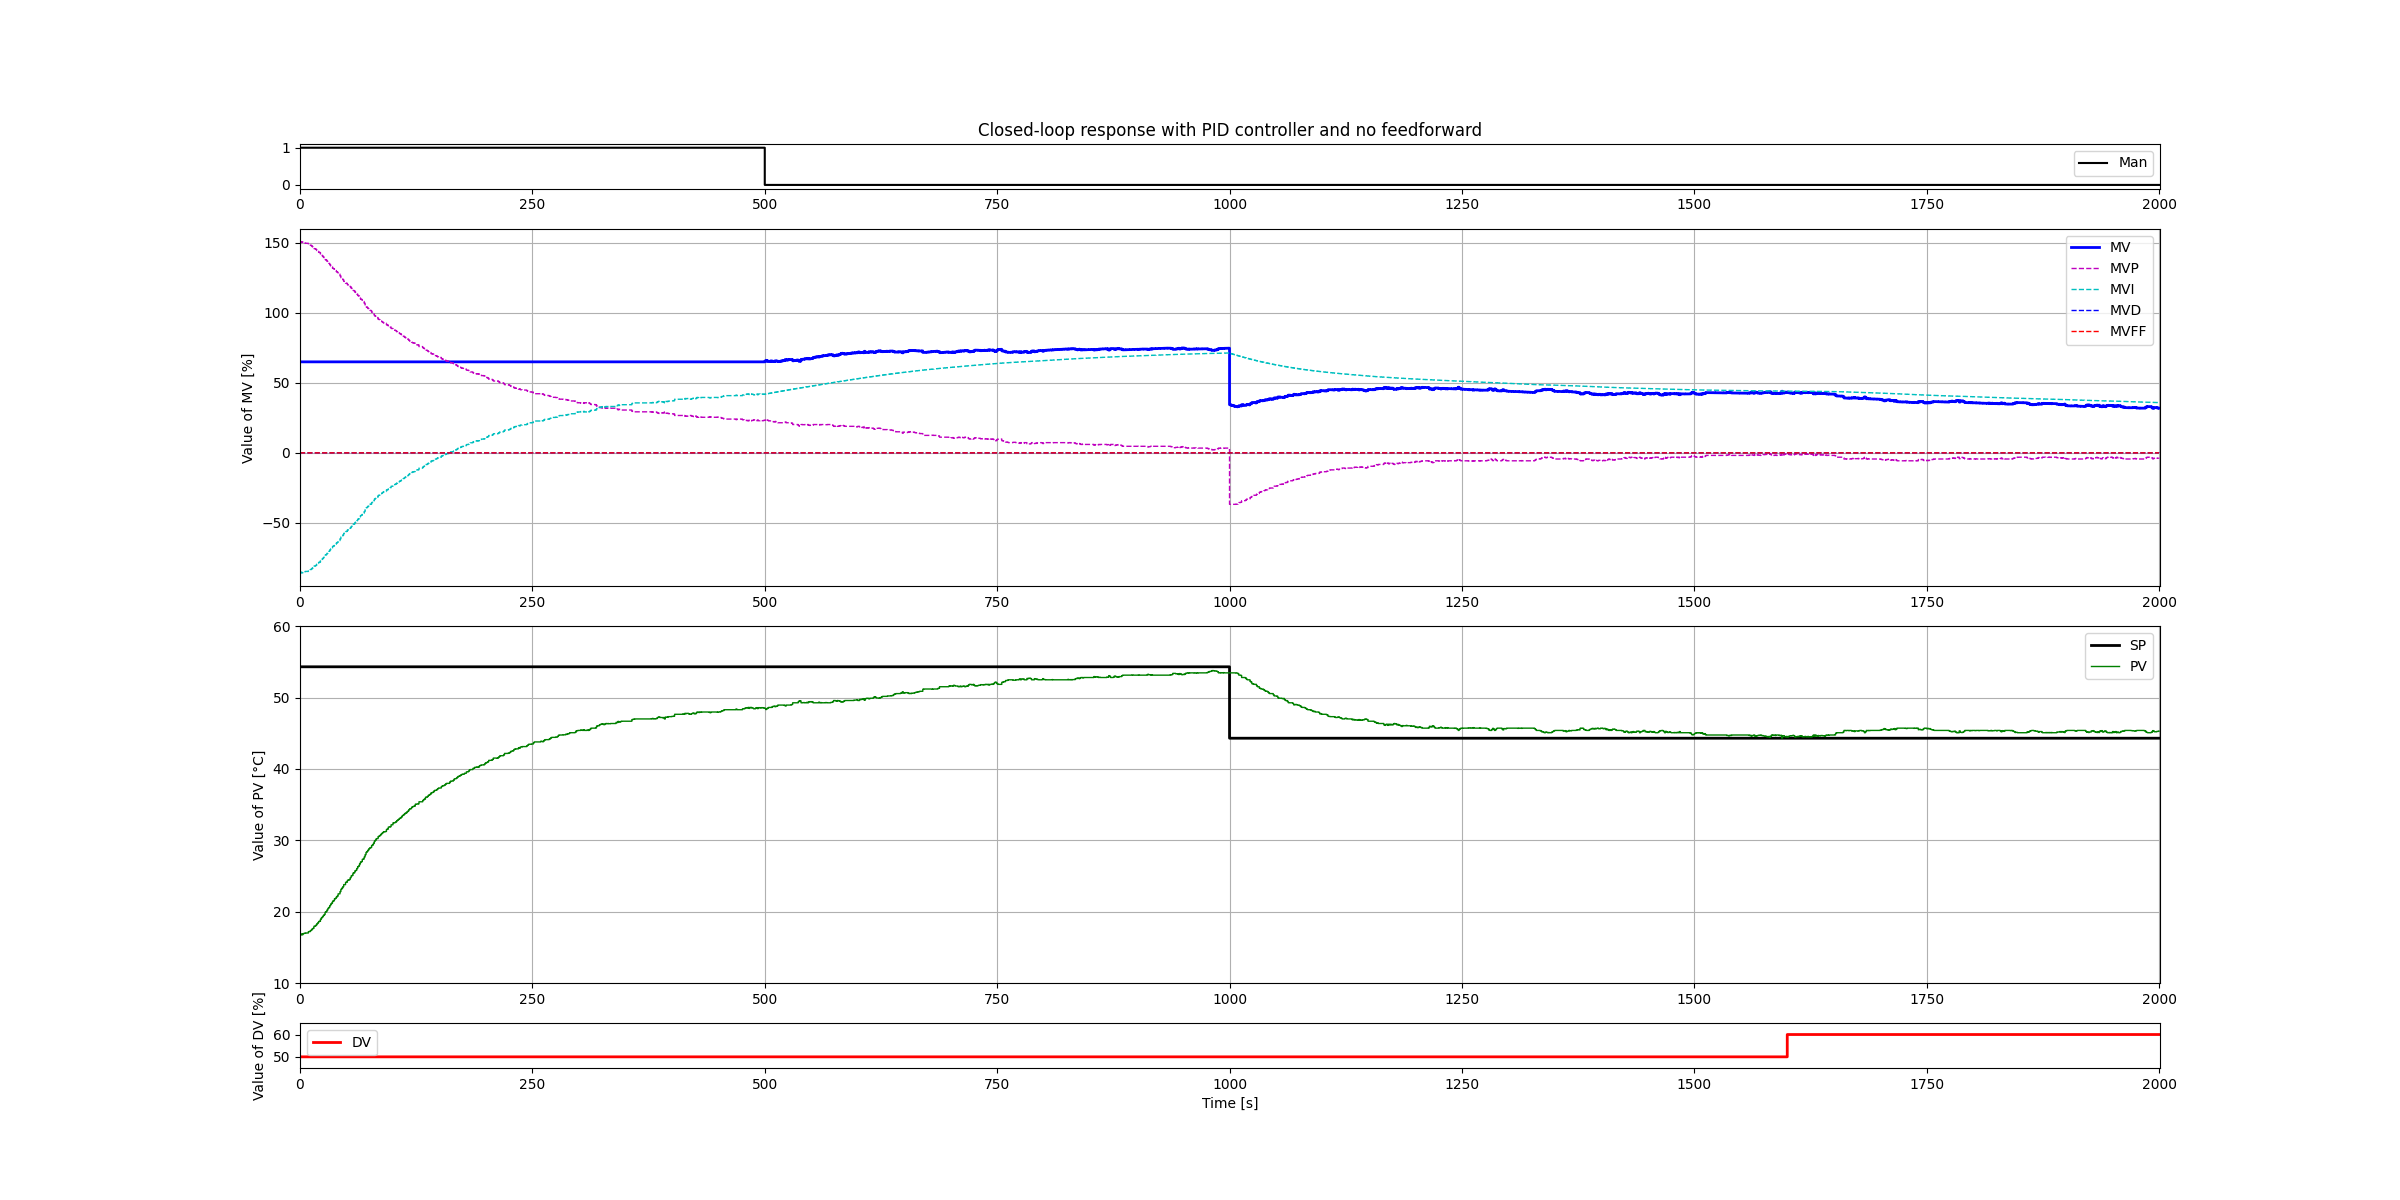
\includegraphics[width=1\textwidth]{../Plots/Experiment_scenario_5_2024-03-30-15h32.png}
	\caption{Données expérimentales du $3^{ème}$ scénario}
	\label{fig:exp_scenario3}
\end{figure}
\begin{figure}[H]
	\centering
	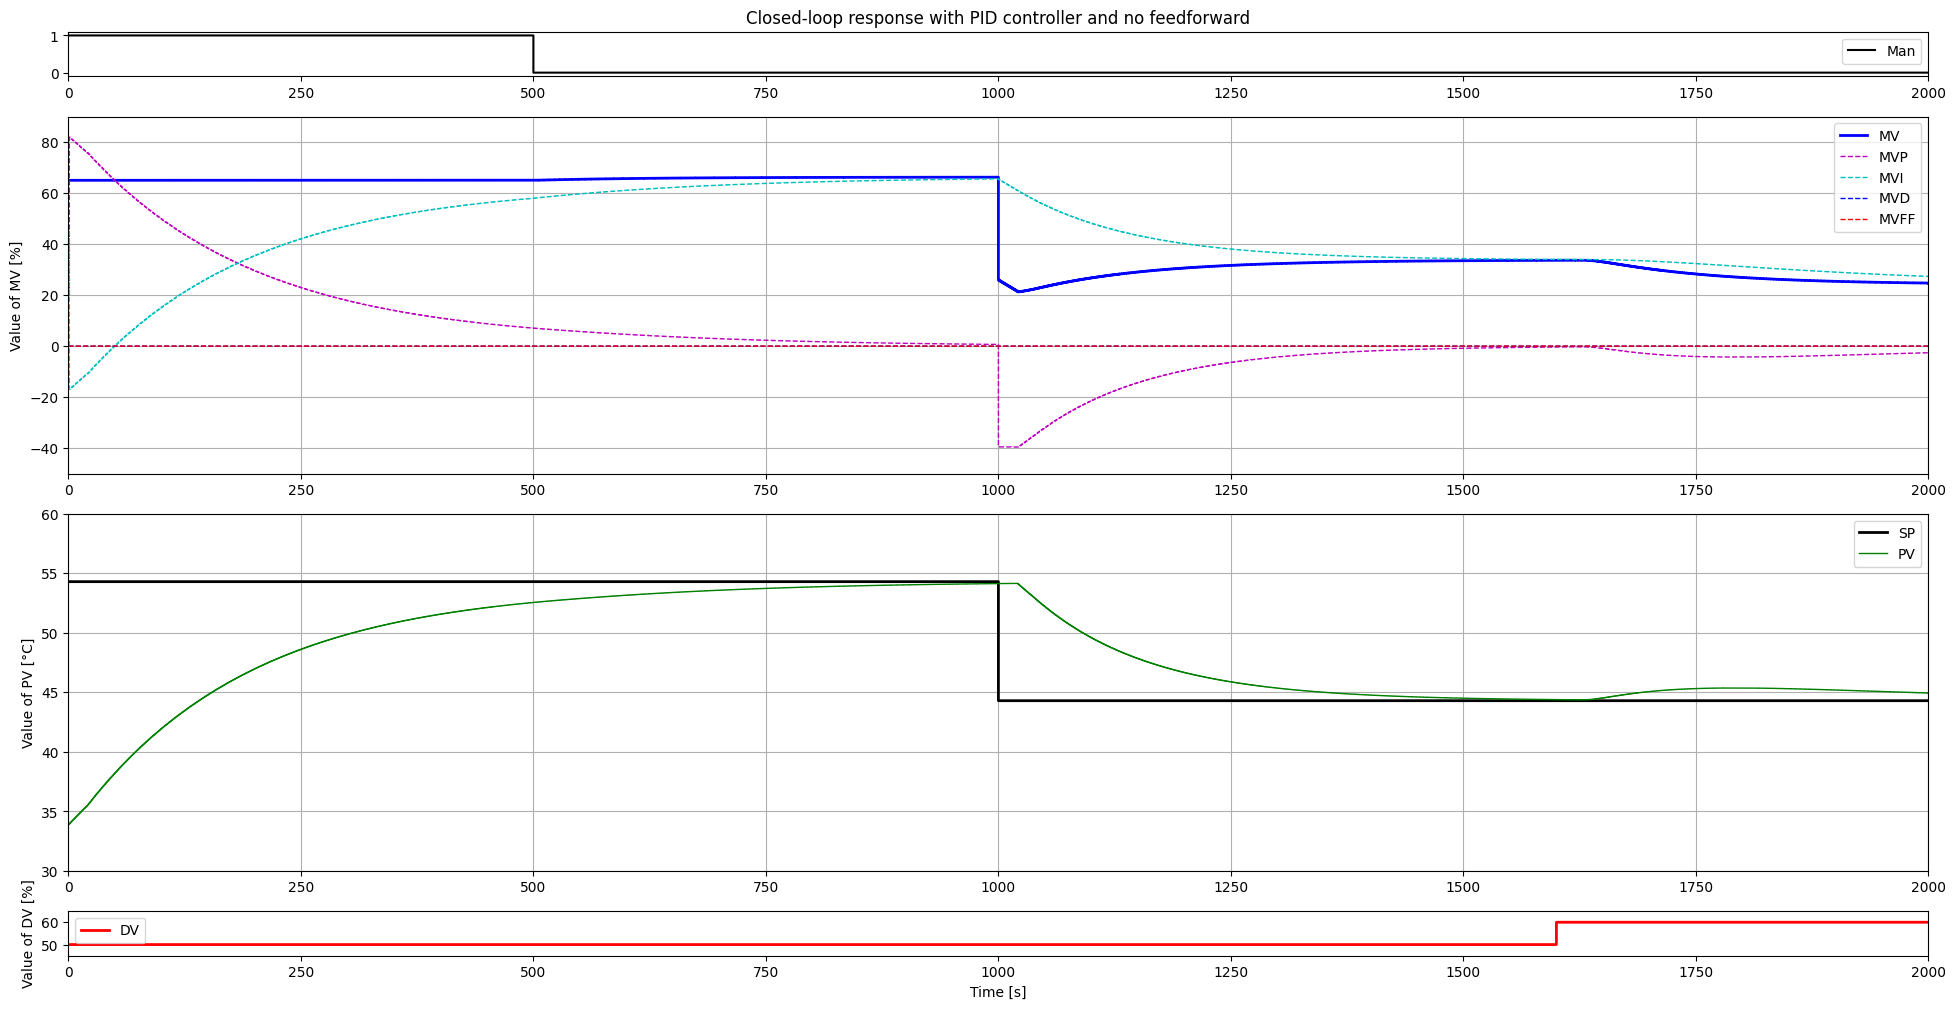
\includegraphics[width=0.8\textwidth]{figures/scenario5.png}
	\caption{Données de la simulation du $3^{ème}$ scénario}
	\label{fig:sim_scenario3}
\end{figure}

Comme pour le $1^{er}$ scénario (\ref{fig:exp_scenario1}), la valeur du $PV$ pour $t = 0s$ est de $\sim 17\degree C$ ce qui cause un retard, par rapport à la simulation, dans l'atteinte de la valeur
de consigne. Ensuite, on observe que le régulateur PID réagit correctement au step de $-10\%$ et atteint la nouvelle valeur de consigne presque en même temps que
pour la simulation. Pour finir, après la perturbation, on observe bien une diminution de $MV$ afin de faire revenir $PV$ à la valeur de consigne. 

\subsection{Scénario 4}

Pour ce scénario, nous avons décidé de répéter l'expérience en changeant la valeur du gamma suite à l'observation de son impact sur les données expérimentales.
Cet impact n'est cependant pas visible sur la simulation.

\subsubsection{$\gamma = 0.5$}

\begin{figure}[H]
	\centering
	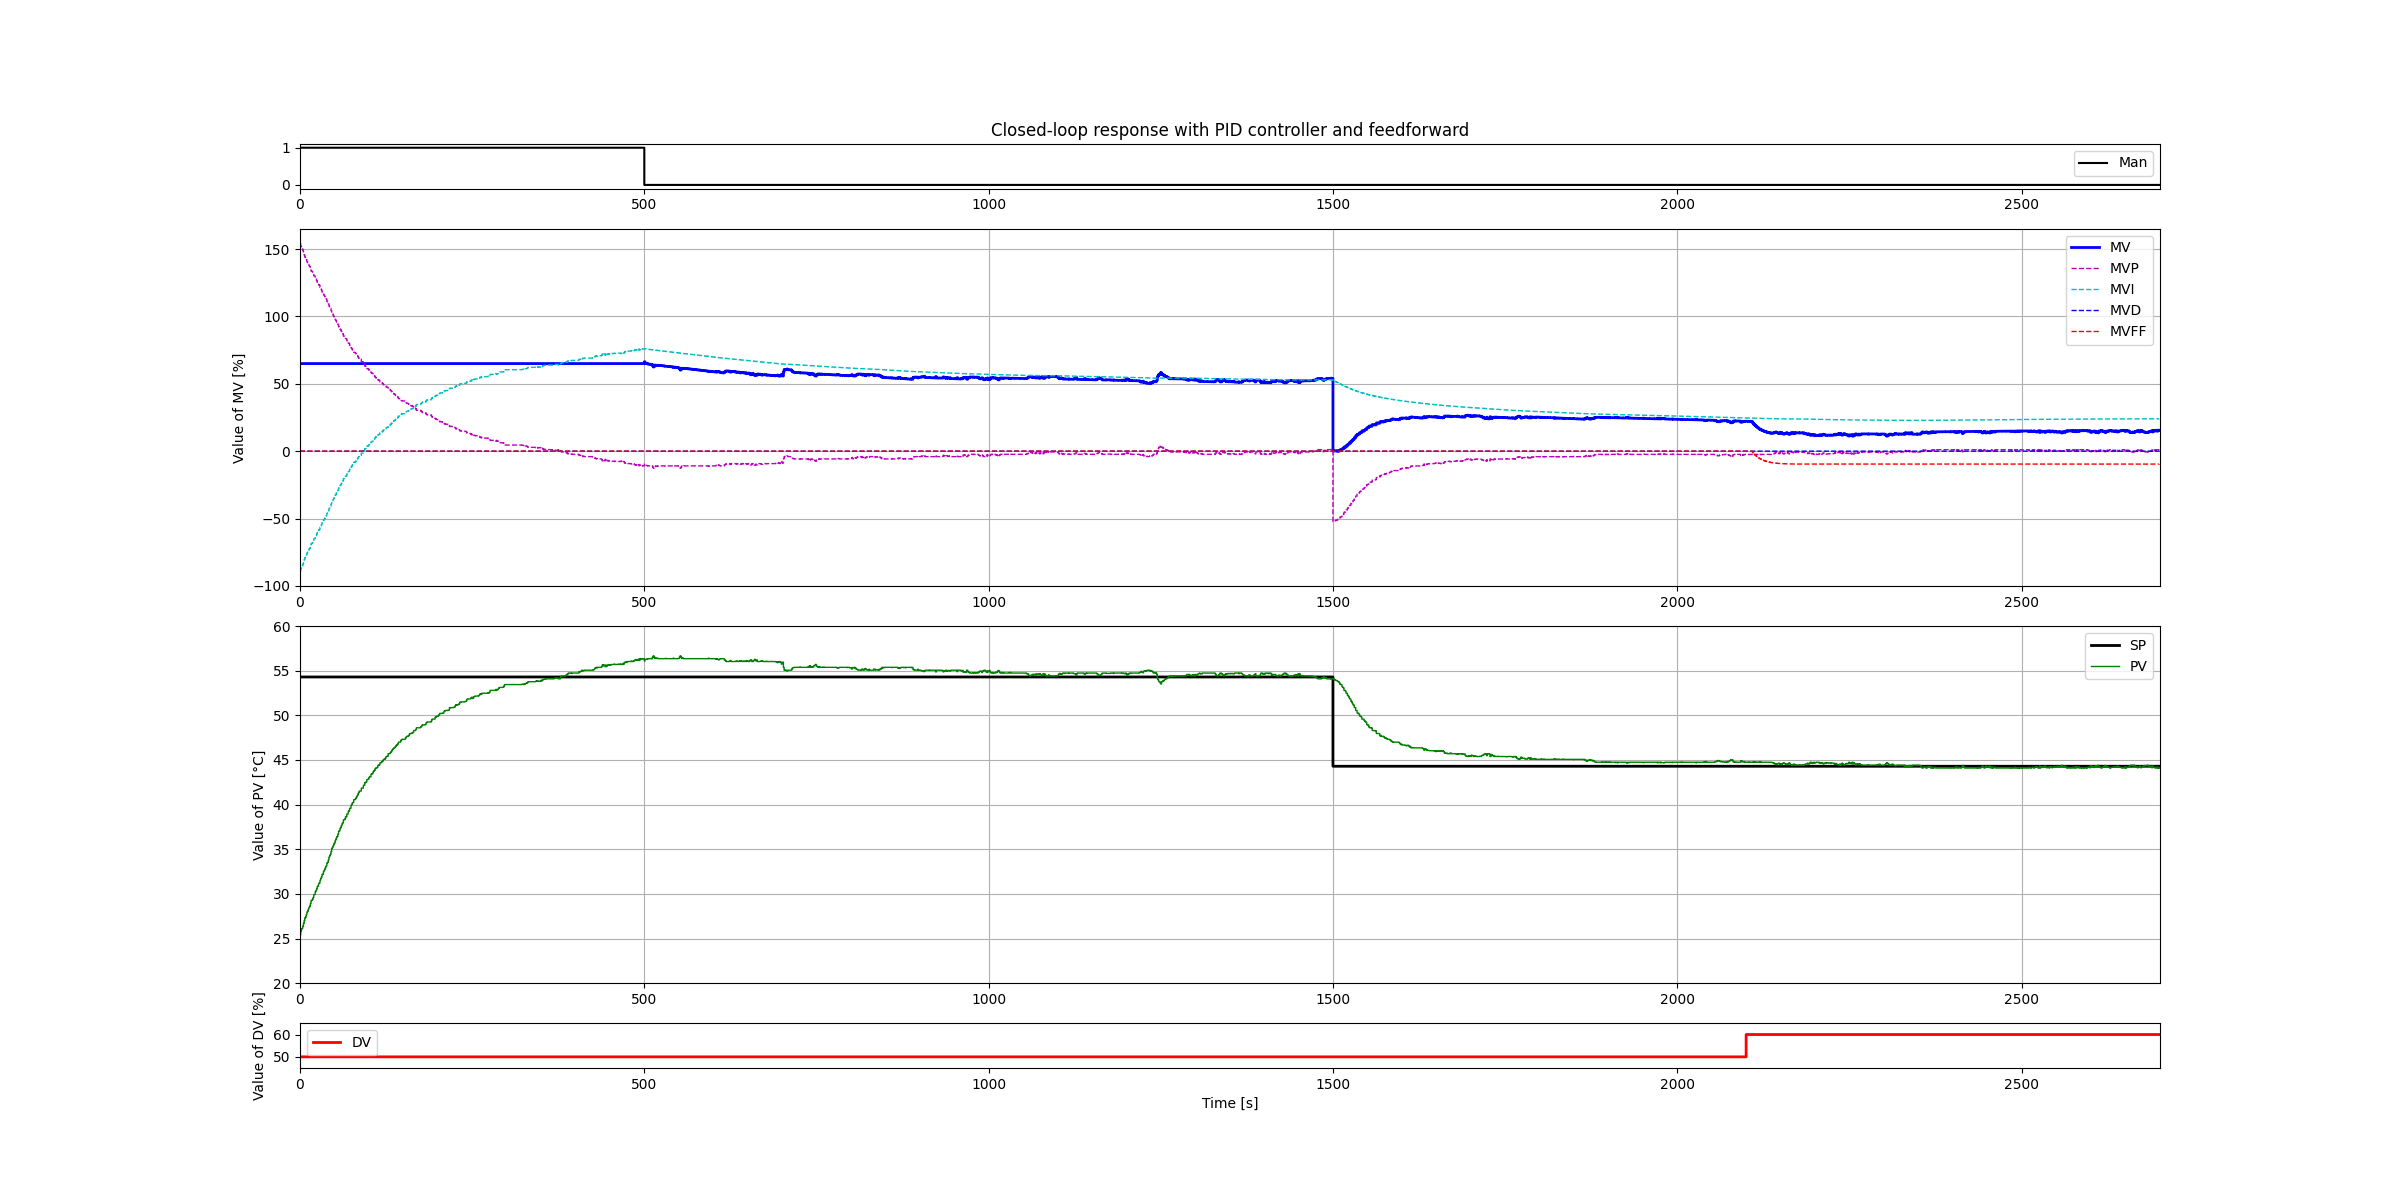
\includegraphics[width=1\textwidth]{../Plots/Experiment_scenario_7_2024-03-29-17h44.png}
	\caption{Données expérimentales du $4^{ème}$ scénario, $\gamma = 0.5$}
	\label{fig:exp_scenario5_0.5}
\end{figure}
\begin{figure}[H]
	\centering
	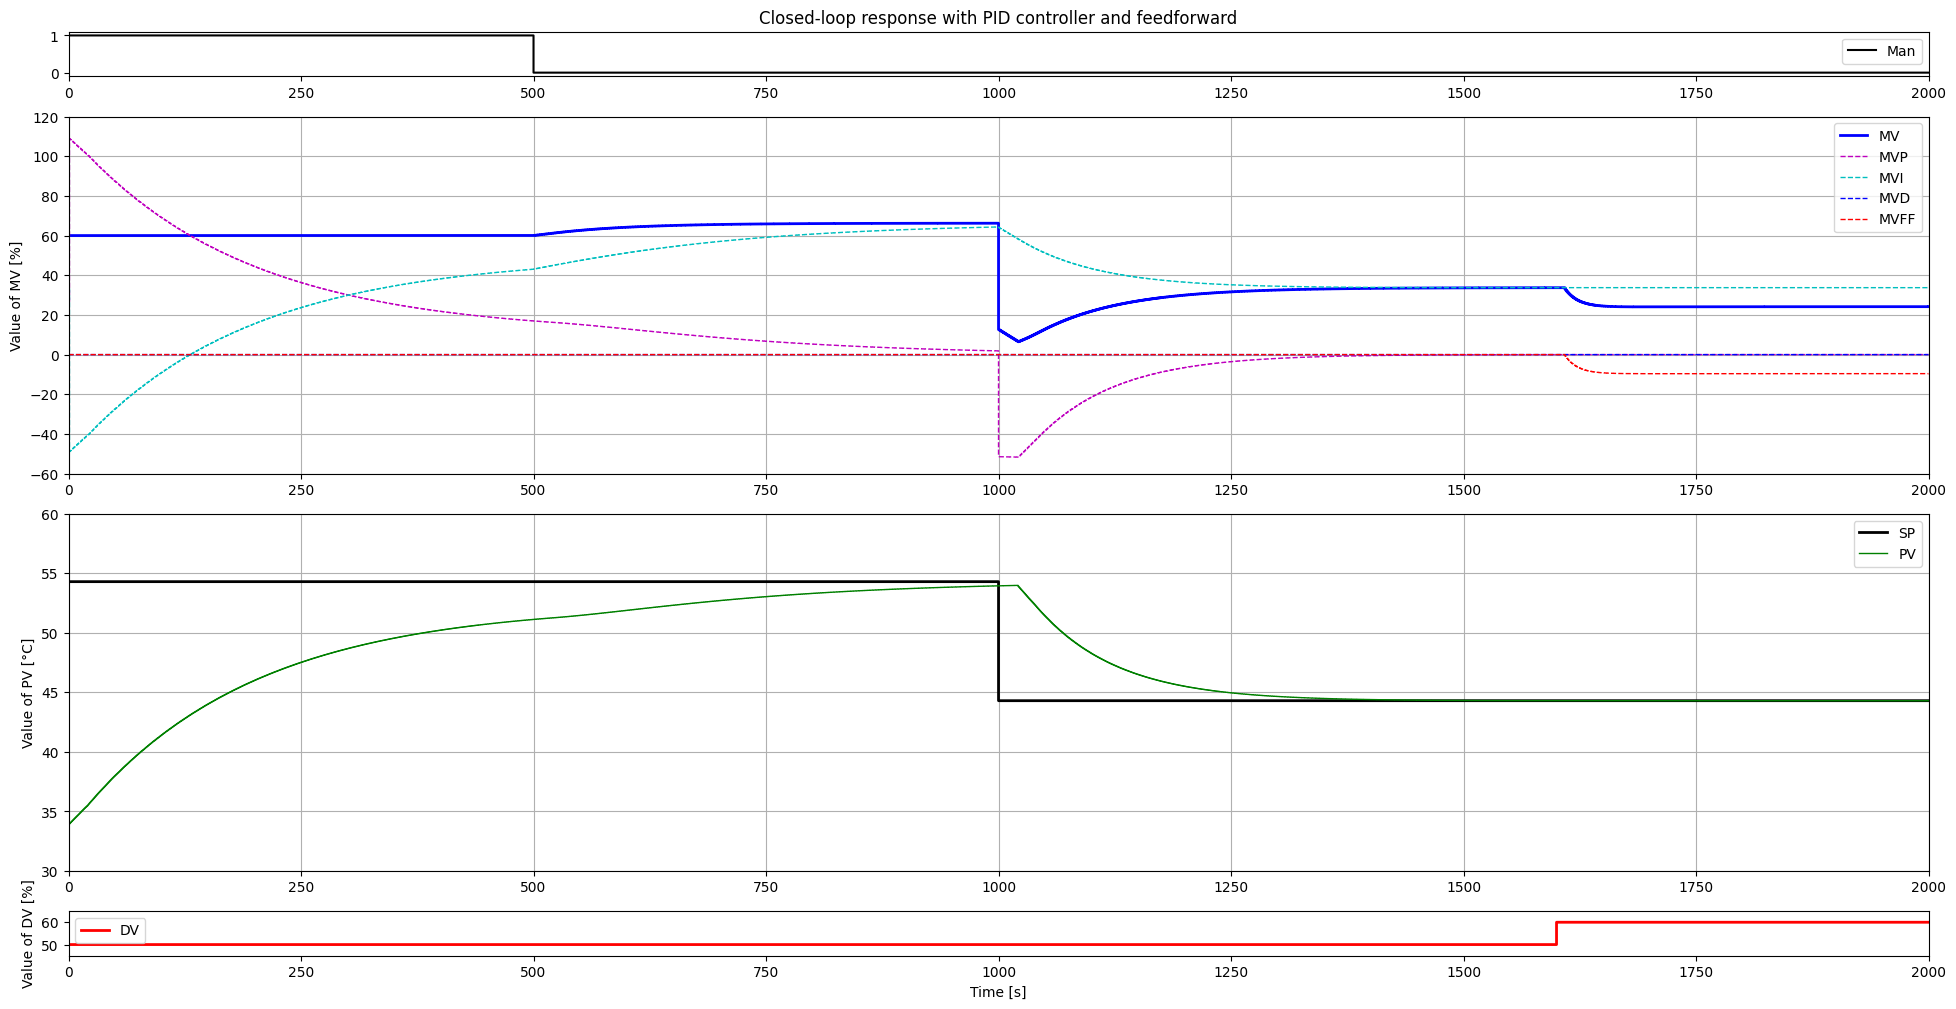
\includegraphics[width=0.8\textwidth]{figures/scenario7.png}
	\caption{Données de la simulation du $4^{ème}$ scénario, $\gamma = 0.5$}
	\label{fig:sim_scenario5_0.5}
\end{figure}

Premièrement, la valeur de $PV$ à $t = 0s$ étant plus élevée que pour tous les scénarios précédents, on observe une convergence de $PV$ vers la valeur de consigne 
plus rapide. Le système présente également un comportement plus proche d'un système du $1^{er}$ ordre. 
\\Par ailleurs, contrairement à ce qui est observé dans la simulation, l'expérience montre un dépassement (overshoot) de la température.
La forme de la courbe de l'expérience diffère beaucoup de celle de la simulation. Cela n'est pas dû à la valeur de gamma puisque l'overshoot aurait alors été également visible dans la simulation. 
L'occurence de l'overshoot dans l'expérience, mais pas dans la simulation ainsi que la grande similitude entre les données expérimentales et simulées dans le 
scénario suivant, suggèrent que cet overshoot pourrait résulter d'une erreur de manipulation lors de l'expérience.
\\Outre l'overshoot, on observe que le régulateur PID réagit correctement à la perturbation puisque $PV$ reste constant malgré le step de $10\%$ sur $DV$.

\subsubsection{$\gamma = 0.7$}

\begin{figure}[H]
	\centering
	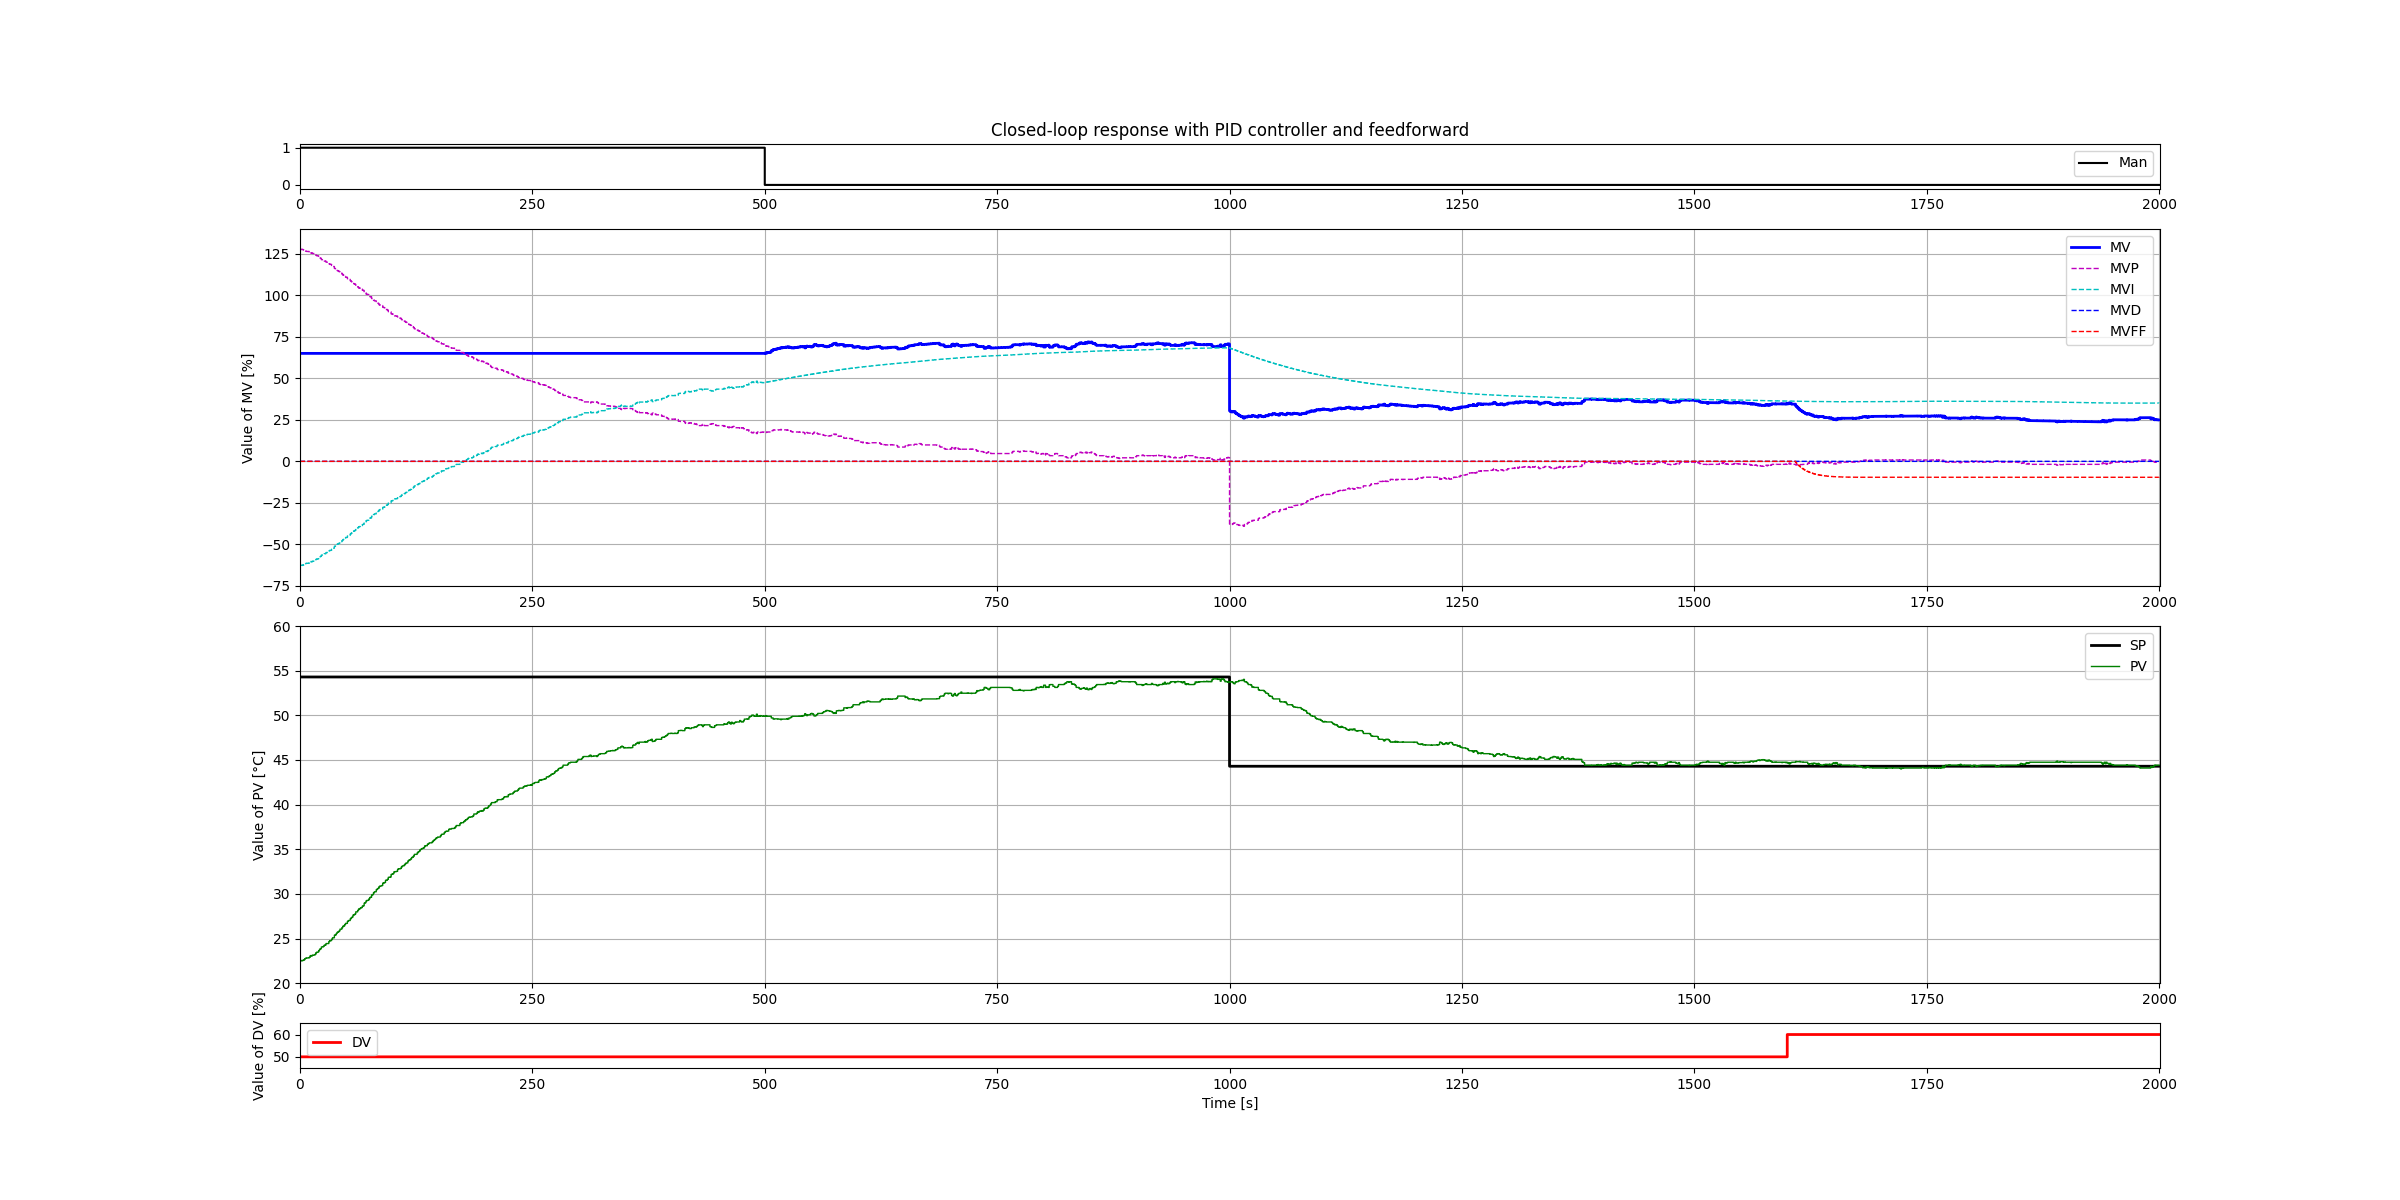
\includegraphics[width=1\textwidth]{../Plots/Experiment_scenario_7_2024-03-29-22h23.png}
	\caption{Données expérimentales du $4^{ème}$ scénario, $\gamma = 0.7$}
	\label{fig:exp_scenario5_0.7}
\end{figure}
\begin{figure}[H]
	\centering
	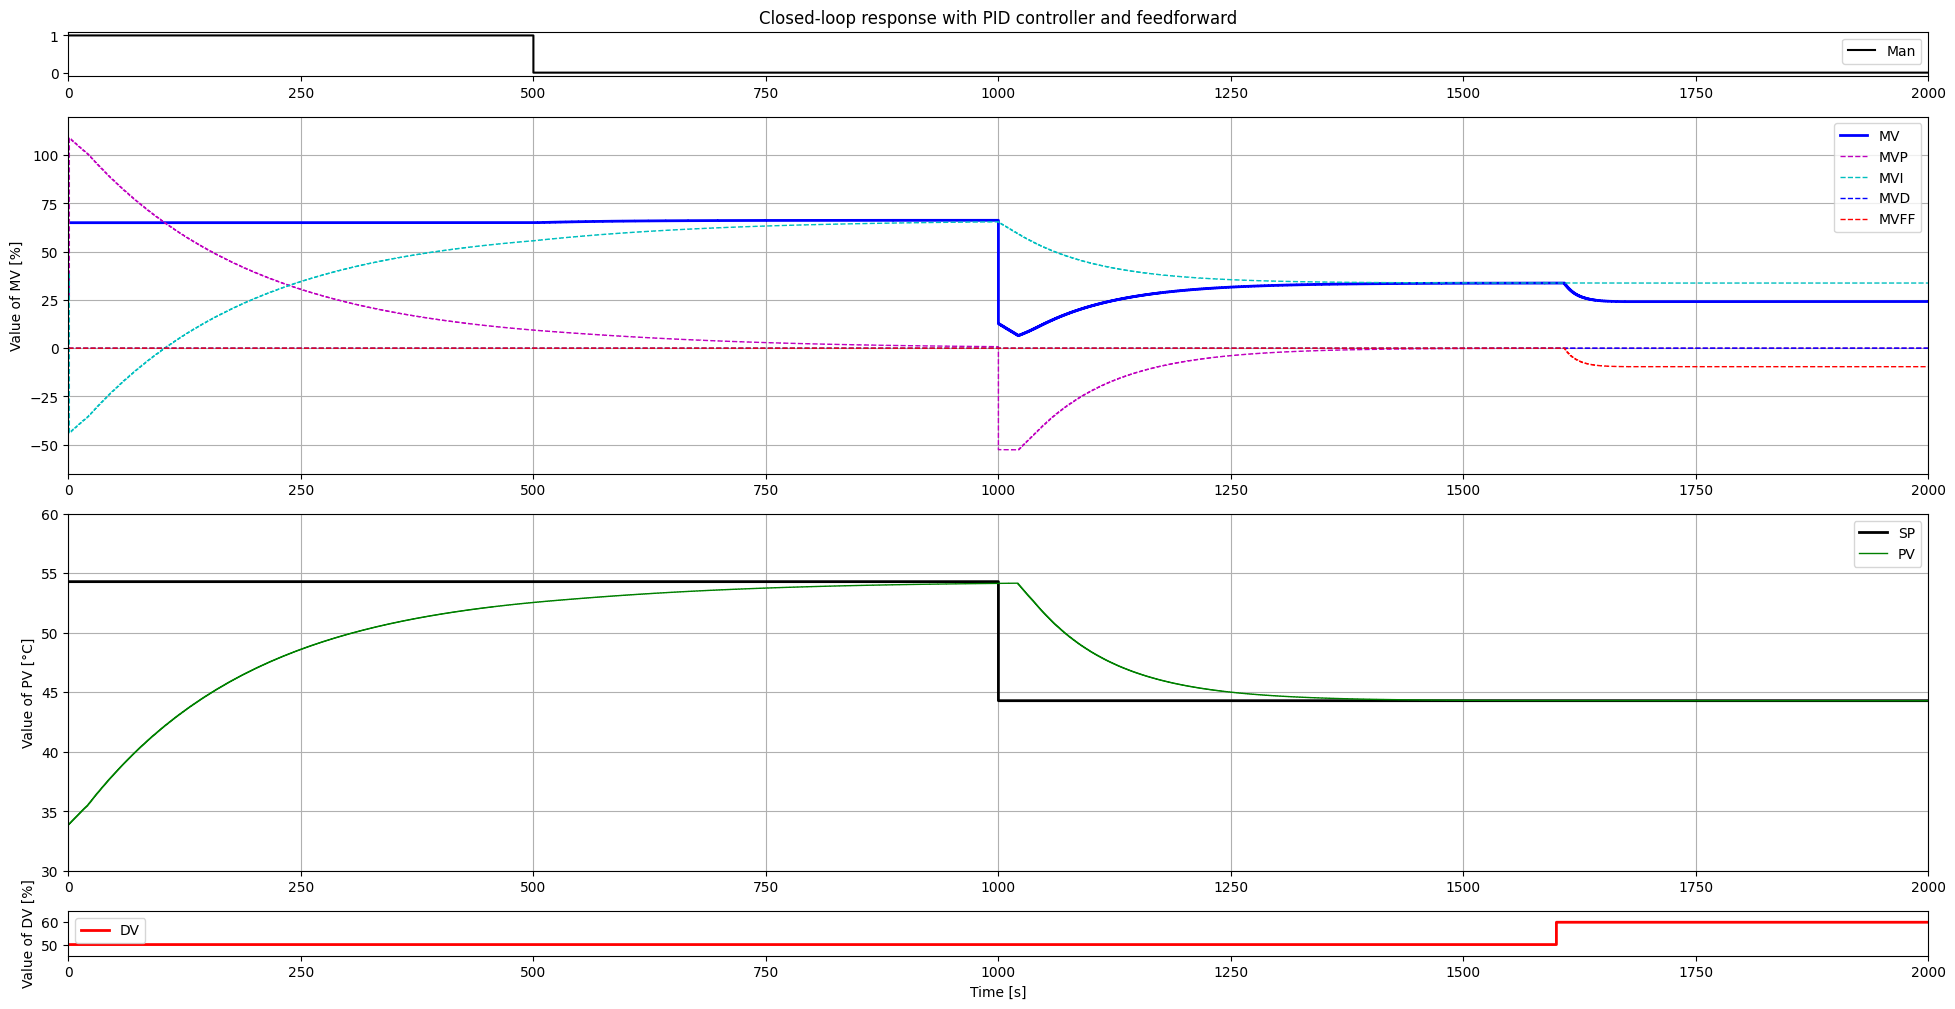
\includegraphics[width=0.8\textwidth]{figures/scenario77.png}
	\caption{Données de la simulation du $4^{ème}$ scénario, $\gamma = 0.7$}
	\label{fig:sim_scenario5_0.7}
\end{figure}

Pour cette dernière expérience, on observe des résultats beaucoup plus cohérents pr rapport à la simulation. Le système réel prend plus de temps à converger
vers la consigne ce qui est dû à la valeur initiale de $PV$ comme discuté précédemment. L'overshoot observé dans le scénario précédent n'est plus présent.
L'augmentation de $\gamma$ peut y avoir contribué puisque cela a comme effet de diminuer ``l'agressivité'' du régulateur en diminuant la constante de gain $K_c$ de celui-ci.
\\Le régulateur PID réagit correctement au changement de consigne et atteint la nouvelle valeur presque en même temps que pour la simulation. 
On peut justement observer l'influence du gamma en comparant ce changement de consigne avec celui où $\gamma = 0.5$ (\ref{fig:exp_scenario5_0.5}). En effet,
la courbe de $PV$ est plus progressive pour $\gamma = 0.7$ que pour $\gamma = 0.5$. Ceci est dû à la diminution de $K_c$ : 
\[T_{CLP} = \gamma\cdot T_{1P}\]
\[\Rightarrow K_c = \frac{1}{K}\,\frac{T_{1P}+T_{2P}}{T_{CLP}+\theta}\]
Et cette diminution de $K_c$ a pour effet de diminuer la valeur de $MV$ à chaque itération du régulateur PID et donc de rendre la réponse du système plus lente.
Pour terminer, le régulateur réagit correctement à la perturbation causée par le step de $10\%$ sur $DV$ puisque, comme pour la simulation, $PV$ reste constant.


%---------- Annexes ----------%
\newpage
\appendix
\section{Méthode graphique pour l'obtention des paramètres d'approximation}
\label{appendix:MV_graphical_method}
\begin{figure}[H]
    \centering
    \includegraphics[width=\textwidth]{../Data/Scanned.pdf}
    \caption{Obtention des paramètres d'approximation pour un step sur MV}
\end{figure}

\end{document}
